%&preformat-disser
\RequirePackage[l2tabu,orthodox]{nag} % Раскомментировав, можно в логе получать рекомендации относительно правильного использования пакетов и предупреждения об устаревших и нерекомендуемых пакетах
% Формат А4, 14pt (ГОСТ Р 7.0.11-2011, 5.3.6)
\documentclass[a4paper,14pt,oneside,openany]{memoir}

%%%%%%%%%%%%%%%%%%%%%%%%%%%%%%%%%%%%%%%%%%%%%%%%%%%%%%
%%%% Файл упрощённых настроек шаблона диссертации %%%%
%%%%%%%%%%%%%%%%%%%%%%%%%%%%%%%%%%%%%%%%%%%%%%%%%%%%%%

%%% Инициализирование переменных, не трогать!  %%%
\newcounter{intvl}
\newcounter{otstup}
\newcounter{contnumeq}
\newcounter{contnumfig}
\newcounter{contnumtab}
\newcounter{pgnum}
\newcounter{chapstyle}
\newcounter{headingdelim}
\newcounter{headingalign}
\newcounter{headingsize}
%%%%%%%%%%%%%%%%%%%%%%%%%%%%%%%%%%%%%%%%%%%%%%%%%%%%%%

%%% Область упрощённого управления оформлением %%%

%% Интервал между заголовками и между заголовком и текстом %%
% Заголовки отделяют от текста сверху и снизу
% тремя интервалами (ГОСТ Р 7.0.11-2011, 5.3.5)
\setcounter{intvl}{3}               % Коэффициент кратности к размеру шрифта

%% Отступы у заголовков в тексте %%
\setcounter{otstup}{0}              % 0 --- без отступа; 1 --- абзацный отступ

%% Нумерация формул, таблиц и рисунков %%
% Нумерация формул
\setcounter{contnumeq}{0}   % 0 --- пораздельно (во введении подряд,
                            %       без номера раздела);
                            % 1 --- сквозная нумерация по всей диссертации
% Нумерация рисунков
\setcounter{contnumfig}{0}  % 0 --- пораздельно (во введении подряд,
                            %       без номера раздела);
                            % 1 --- сквозная нумерация по всей диссертации
% Нумерация таблиц
\setcounter{contnumtab}{1}  % 0 --- пораздельно (во введении подряд,
                            %       без номера раздела);
                            % 1 --- сквозная нумерация по всей диссертации

%% Оглавление %%
\setcounter{pgnum}{1}       % 0 --- номера страниц никак не обозначены;
                            % 1 --- Стр. над номерами страниц (дважды
                            %       компилировать после изменения настройки)
\settocdepth{subsection}    % до какого уровня подразделов выносить в оглавление
\setsecnumdepth{subsection} % до какого уровня нумеровать подразделы


%% Текст и форматирование заголовков %%
\setcounter{chapstyle}{1}     % 0 --- разделы только под номером;
                              % 1 --- разделы с названием "Глава" перед номером
\setcounter{headingdelim}{1}  % 0 --- номер отделен пропуском в 1em или \quad;
                              % 1 --- номера разделов и приложений отделены
                              %       точкой с пробелом, подразделы пропуском
                              %       без точки;
                              % 2 --- номера разделов, подразделов и приложений
                              %       отделены точкой с пробелом.

%% Выравнивание заголовков в тексте %%
\setcounter{headingalign}{0}  % 0 --- по центру;
                              % 1 --- по левому краю

%% Размеры заголовков в тексте %%
\setcounter{headingsize}{0}   % 0 --- по ГОСТ, все всегда 14 пт;
                              % 1 --- пропорционально изменяющийся размер
                              %       в зависимости от базового шрифта

%% Подпись таблиц %%

% Смещение строк подписи после первой строки
\newcommand{\tabindent}{0cm}

% Тип форматирования заголовка таблицы:
% plain --- название и текст в одной строке
% split --- название и текст в разных строках
\newcommand{\tabformat}{plain}

%%% Настройки форматирования таблицы `plain`

% Выравнивание по центру подписи, состоящей из одной строки:
% true  --- выравнивать
% false --- не выравнивать
\newcommand{\tabsinglecenter}{false}

% Выравнивание подписи таблиц:
% justified   --- выравнивать как обычный текст («по ширине»)
% centering   --- выравнивать по центру
% centerlast  --- выравнивать по центру только последнюю строку
% centerfirst --- выравнивать по центру только первую строку (не рекомендуется)
% raggedleft  --- выравнивать по правому краю
% raggedright --- выравнивать по левому краю
\newcommand{\tabjust}{justified}

% Разделитель записи «Таблица #» и названия таблицы
\newcommand{\tablabelsep}{~\cyrdash\ }

%%% Настройки форматирования таблицы `split`

% Положение названия таблицы:
% \centering   --- выравнивать по центру
% \raggedleft  --- выравнивать по правому краю
% \raggedright --- выравнивать по левому краю
\newcommand{\splitformatlabel}{\raggedleft}

% Положение текста подписи:
% \centering   --- выравнивать по центру
% \raggedleft  --- выравнивать по правому краю
% \raggedright --- выравнивать по левому краю
\newcommand{\splitformattext}{\raggedright}

%% Подпись рисунков %%
%Разделитель записи «Рисунок #» и названия рисунка
\newcommand{\figlabelsep}{~\cyrdash\ }  % (ГОСТ 2.105, 4.3.1)
                                        % "--- здесь не работает

%%% Цвета гиперссылок %%%
% Latex color definitions: http://latexcolor.com/
%\definecolor{linkcolor}{rgb}{0.9,0,0}
%\definecolor{citecolor}{rgb}{0,0.6,0}
%\definecolor{urlcolor}{rgb}{0,0,1}
\definecolor{linkcolor}{rgb}{0,0,0} %black
\definecolor{citecolor}{rgb}{0,0,0} %black
\definecolor{urlcolor}{rgb}{0,0,0} %black
            % общие настройки шаблона
\input{common/packages}         % Пакеты общие для диссертации и автореферата
\synopsisfalse                      % Этот документ --- не автореферат
\input{Dissertation/dispackages}    % Пакеты для диссертации
\input{Dissertation/userpackages}   % Пакеты для специфических пользовательских задач

%%%%%%%%%%%%%%%%%%%%%%%%%%%%%%%%%%%%%%%%%%%%%%%%%%%%%%
%%%% Файл упрощённых настроек шаблона диссертации %%%%
%%%%%%%%%%%%%%%%%%%%%%%%%%%%%%%%%%%%%%%%%%%%%%%%%%%%%%

%%% Инициализирование переменных, не трогать!  %%%
\newcounter{intvl}
\newcounter{otstup}
\newcounter{contnumeq}
\newcounter{contnumfig}
\newcounter{contnumtab}
\newcounter{pgnum}
\newcounter{chapstyle}
\newcounter{headingdelim}
\newcounter{headingalign}
\newcounter{headingsize}
%%%%%%%%%%%%%%%%%%%%%%%%%%%%%%%%%%%%%%%%%%%%%%%%%%%%%%

%%% Область упрощённого управления оформлением %%%

%% Интервал между заголовками и между заголовком и текстом %%
% Заголовки отделяют от текста сверху и снизу
% тремя интервалами (ГОСТ Р 7.0.11-2011, 5.3.5)
\setcounter{intvl}{3}               % Коэффициент кратности к размеру шрифта

%% Отступы у заголовков в тексте %%
\setcounter{otstup}{0}              % 0 --- без отступа; 1 --- абзацный отступ

%% Нумерация формул, таблиц и рисунков %%
% Нумерация формул
\setcounter{contnumeq}{0}   % 0 --- пораздельно (во введении подряд,
                            %       без номера раздела);
                            % 1 --- сквозная нумерация по всей диссертации
% Нумерация рисунков
\setcounter{contnumfig}{0}  % 0 --- пораздельно (во введении подряд,
                            %       без номера раздела);
                            % 1 --- сквозная нумерация по всей диссертации
% Нумерация таблиц
\setcounter{contnumtab}{1}  % 0 --- пораздельно (во введении подряд,
                            %       без номера раздела);
                            % 1 --- сквозная нумерация по всей диссертации

%% Оглавление %%
\setcounter{pgnum}{1}       % 0 --- номера страниц никак не обозначены;
                            % 1 --- Стр. над номерами страниц (дважды
                            %       компилировать после изменения настройки)
\settocdepth{subsection}    % до какого уровня подразделов выносить в оглавление
\setsecnumdepth{subsection} % до какого уровня нумеровать подразделы


%% Текст и форматирование заголовков %%
\setcounter{chapstyle}{1}     % 0 --- разделы только под номером;
                              % 1 --- разделы с названием "Глава" перед номером
\setcounter{headingdelim}{1}  % 0 --- номер отделен пропуском в 1em или \quad;
                              % 1 --- номера разделов и приложений отделены
                              %       точкой с пробелом, подразделы пропуском
                              %       без точки;
                              % 2 --- номера разделов, подразделов и приложений
                              %       отделены точкой с пробелом.

%% Выравнивание заголовков в тексте %%
\setcounter{headingalign}{0}  % 0 --- по центру;
                              % 1 --- по левому краю

%% Размеры заголовков в тексте %%
\setcounter{headingsize}{0}   % 0 --- по ГОСТ, все всегда 14 пт;
                              % 1 --- пропорционально изменяющийся размер
                              %       в зависимости от базового шрифта

%% Подпись таблиц %%

% Смещение строк подписи после первой строки
\newcommand{\tabindent}{0cm}

% Тип форматирования заголовка таблицы:
% plain --- название и текст в одной строке
% split --- название и текст в разных строках
\newcommand{\tabformat}{plain}

%%% Настройки форматирования таблицы `plain`

% Выравнивание по центру подписи, состоящей из одной строки:
% true  --- выравнивать
% false --- не выравнивать
\newcommand{\tabsinglecenter}{false}

% Выравнивание подписи таблиц:
% justified   --- выравнивать как обычный текст («по ширине»)
% centering   --- выравнивать по центру
% centerlast  --- выравнивать по центру только последнюю строку
% centerfirst --- выравнивать по центру только первую строку (не рекомендуется)
% raggedleft  --- выравнивать по правому краю
% raggedright --- выравнивать по левому краю
\newcommand{\tabjust}{justified}

% Разделитель записи «Таблица #» и названия таблицы
\newcommand{\tablabelsep}{~\cyrdash\ }

%%% Настройки форматирования таблицы `split`

% Положение названия таблицы:
% \centering   --- выравнивать по центру
% \raggedleft  --- выравнивать по правому краю
% \raggedright --- выравнивать по левому краю
\newcommand{\splitformatlabel}{\raggedleft}

% Положение текста подписи:
% \centering   --- выравнивать по центру
% \raggedleft  --- выравнивать по правому краю
% \raggedright --- выравнивать по левому краю
\newcommand{\splitformattext}{\raggedright}

%% Подпись рисунков %%
%Разделитель записи «Рисунок #» и названия рисунка
\newcommand{\figlabelsep}{~\cyrdash\ }  % (ГОСТ 2.105, 4.3.1)
                                        % "--- здесь не работает

%%% Цвета гиперссылок %%%
% Latex color definitions: http://latexcolor.com/
%\definecolor{linkcolor}{rgb}{0.9,0,0}
%\definecolor{citecolor}{rgb}{0,0.6,0}
%\definecolor{urlcolor}{rgb}{0,0,1}
\definecolor{linkcolor}{rgb}{0,0,0} %black
\definecolor{citecolor}{rgb}{0,0,0} %black
\definecolor{urlcolor}{rgb}{0,0,0} %black
      % Упрощённые настройки шаблона

\input{common/newnames}         % Новые переменные, для всего проекта

%%% Основные сведения %%%
\newcommand{\thesisAuthorLastName}{Антонов}
\newcommand{\thesisAuthorOtherNames}{Илья Денисович}
\newcommand{\thesisAuthorInitials}{И.\,Д.}
\newcommand{\thesisAuthor}             % Диссертация, ФИО автора
{%
    \texorpdfstring{% \texorpdfstring takes two arguments and uses the first for (La)TeX and the second for pdf
        \thesisAuthorLastName~\thesisAuthorOtherNames% так будет отображаться на титульном листе или в тексте, где будет использоваться переменная
    }{%
        \thesisAuthorLastName, \thesisAuthorOtherNames% эта запись для свойств pdf-файла. В таком виде, если pdf будет обработан программами для сбора библиографических сведений, будет правильно представлена фамилия.
    }
}
\newcommand{\thesisAuthorShort}        % Диссертация, ФИО автора инициалами
{\thesisAuthorInitials~\thesisAuthorLastName}
%\newcommand{\thesisUdk}                % Диссертация, УДК
%{\fixme{xxx.xxx}}
\newcommand{\thesisTitle}              % Диссертация, название
{Проблемы управления нелинейными волновыми процессами в механических системах и численные методы их решения}
\newcommand{\thesisSpecialtyNumber}    % Диссертация, специальность, номер
{01.02.04}
\newcommand{\thesisSpecialtyTitle}     % Диссертация, специальность, название (название взято с сайта ВАК для примера)
{Механика деформируемого теврдого тела}
%% \newcommand{\thesisSpecialtyTwoNumber} % Диссертация, вторая специальность, номер
%% {\fixme{XX.XX.XX}}
%% \newcommand{\thesisSpecialtyTwoTitle}  % Диссертация, вторая специальность, название
%% {\fixme{Теория и~методика физического воспитания, спортивной тренировки,
%% оздоровительной и~адаптивной физической культуры}}
\newcommand{\thesisDegree}             % Диссертация, ученая степень
{кандидата физико-математических наук}
\newcommand{\thesisDegreeShort}        % Диссертация, ученая степень, краткая запись
{канд. физ.-мат. наук}
\newcommand{\thesisCity}               % Диссертация, город написания диссертации
{Санкт-Петербург}
\newcommand{\thesisYear}               % Диссертация, год написания диссертации
{\the\year}
\newcommand{\thesisOrganization}       % Диссертация, организация
{Федеральное государственное бюджетное учреждение науки <<Институт проблем машиноведения Российской академии наук <<ИПМаш РАН>>}
\newcommand{\thesisOrganizationShort}  % Диссертация, краткое название организации для доклада
{ИПМаш РАН}

\newcommand{\thesisInOrganization}     % Диссертация, организация в предложном падеже: Работа выполнена в ...
{институте проблем машиноведения Российской академии наук}

%% \newcommand{\supervisorDead}{}           % Рисовать рамку вокруг фамилии
\newcommand{\supervisorFio}              % Научный руководитель, ФИО
{Порубов Алексей Викторович}
\newcommand{\supervisorRegalia}          % Научный руководитель, регалии
{профессор, д-р~физ.-мат. наук}
\newcommand{\supervisorFioShort}         % Научный руководитель, ФИО
{А.\,В.~Порубов}
\newcommand{\supervisorRegaliaShort}     % Научный руководитель, регалии
{проф..,~д.ф.-м.н.}

%% \newcommand{\supervisorTwoDead}{}        % Рисовать рамку вокруг фамилии
%% \newcommand{\supervisorTwoFio}           % Второй научный руководитель, ФИО
%% {\fixme{Фамилия Имя Отчество}}
%% \newcommand{\supervisorTwoRegalia}       % Второй научный руководитель, регалии
%% {\fixme{уч. степень, уч. звание}}
%% \newcommand{\supervisorTwoFioShort}      % Второй научный руководитель, ФИО
%% {\fixme{И.\,О.~Фамилия}}
%% \newcommand{\supervisorTwoRegaliaShort}  % Второй научный руководитель, регалии
%% {\fixme{уч.~ст.,~уч.~зв.}}

\newcommand{\opponentOneFio}           % Оппонент 1, ФИО
{\fixme{Фамилия Имя Отчество}}
\newcommand{\opponentOneRegalia}       % Оппонент 1, регалии
{\fixme{доктор физико-математических наук, профессор}}
\newcommand{\opponentOneJobPlace}      % Оппонент 1, место работы
{\fixme{Не очень длинное название для места работы}}
\newcommand{\opponentOneJobPost}       % Оппонент 1, должность
{\fixme{старший научный сотрудник}}

\newcommand{\opponentTwoFio}           % Оппонент 2, ФИО
{\fixme{Фамилия Имя Отчество}}
\newcommand{\opponentTwoRegalia}       % Оппонент 2, регалии
{\fixme{кандидат физико-математических наук}}
\newcommand{\opponentTwoJobPlace}      % Оппонент 2, место работы
{\fixme{Основное место работы c длинным длинным длинным длинным названием}}
\newcommand{\opponentTwoJobPost}       % Оппонент 2, должность
{\fixme{старший научный сотрудник}}

%% \newcommand{\opponentThreeFio}         % Оппонент 3, ФИО
%% {\fixme{Фамилия Имя Отчество}}
%% \newcommand{\opponentThreeRegalia}     % Оппонент 3, регалии
%% {\fixme{кандидат физико-математических наук}}
%% \newcommand{\opponentThreeJobPlace}    % Оппонент 3, место работы
%% {\fixme{Основное место работы c длинным длинным длинным длинным названием}}
%% \newcommand{\opponentThreeJobPost}     % Оппонент 3, должность
%% {\fixme{старший научный сотрудник}}

%% \newcommand{\leadingOrganizationTitle} % Ведущая организация, дополнительные строки. Удалить, чтобы не отображать в автореферате
%% {\fixme{Федеральное государственное бюджетное образовательное учреждение высшего
%% профессионального образования с~длинным длинным длинным длинным названием}}

\newcommand{\defenseDate}              % Защита, дата
{\fixme{DD mmmmmmmm YYYY~г.~в~XX часов}}
\newcommand{\defenseCouncilNumber}     % Защита, номер диссертационного совета
{Д\,002.075.01}
\newcommand{\defenseCouncilTitle}      % Защита, учреждение диссертационного совета
{Институт проблем машиноведения Российской академии наук}
\newcommand{\defenseCouncilAddress}    % Защита, адрес учреждение диссертационного совета
{199178, г.Санкт-Петербург, Большой проспект В.О., д.61}
\newcommand{\defenseCouncilPhone}      % Телефон для справок
{+7~(812)~321-47-71}

\newcommand{\defenseSecretaryFio}      % Секретарь диссертационного совета, ФИО
{\fixme{Фамилия Имя Отчество}}
\newcommand{\defenseSecretaryRegalia}  % Секретарь диссертационного совета, регалии
{\fixme{д-р~физ.-мат. наук}}            % Для сокращений есть ГОСТы, например: ГОСТ Р 7.0.12-2011 + http://base.garant.ru/179724/#block_30000

\newcommand{\synopsisLibrary}          % Автореферат, название библиотеки
{\fixme{Название библиотеки}}
\newcommand{\synopsisDate}             % Автореферат, дата рассылки
{\fixme{DD mmmmmmmm}\the\year~года}

% To avoid conflict with beamer class use \providecommand
\providecommand{\keywords}%            % Ключевые слова для метаданных PDF диссертации и автореферата
{}
             % Основные сведения
\input{common/fonts}            % Определение шрифтов (частичное)
%%% Шаблон %%%
\DeclareRobustCommand{\fixme}{\textcolor{black}}  % решаем проблему превращения
                                % названия цвета в результате \MakeUppercase,
                                % http://tex.stackexchange.com/a/187930,
                                % \DeclareRobustCommand protects \fixme
                                % from expanding inside \MakeUppercase
\AtBeginDocument{%
    \setlength{\parindent}{2.5em}                   % Абзацный отступ. Должен быть одинаковым по всему тексту и равен пяти знакам (ГОСТ Р 7.0.11-2011, 5.3.7).
}

%%% Таблицы %%%
\DeclareCaptionLabelSeparator{tabsep}{\tablabelsep} % нумерация таблиц
\DeclareCaptionFormat{split}{\splitformatlabel#1\par\splitformattext#3}

\captionsetup[table]{
        format=\tabformat,                % формат подписи (plain|hang)
        font=normal,                      % нормальные размер, цвет, стиль шрифта
        skip=.0pt,                        % отбивка под подписью
        parskip=.0pt,                     % отбивка между параграфами подписи
        position=above,                   % положение подписи
        justification=\tabjust,           % центровка
        indent=\tabindent,                % смещение строк после первой
        labelsep=tabsep,                  % разделитель
        singlelinecheck=\tabsinglecenter, % не выравнивать по центру, если умещается в одну строку
}

%%% Рисунки %%%
\DeclareCaptionLabelSeparator{figsep}{\figlabelsep} % нумерация рисунков

\captionsetup[figure]{
        format=plain,                     % формат подписи (plain|hang)
        font=normal,                      % нормальные размер, цвет, стиль шрифта
        skip=.0pt,                        % отбивка под подписью
        parskip=.0pt,                     % отбивка между параграфами подписи
        position=below,                   % положение подписи
        singlelinecheck=true,             % выравнивание по центру, если умещается в одну строку
        justification=centerlast,         % центровка
        labelsep=figsep,                  % разделитель
}

%%% Подписи подрисунков %%%
\DeclareCaptionSubType{figure}
\renewcommand\thesubfigure{\asbuk{subfigure}} % нумерация подрисунков
\ifsynopsis
\DeclareCaptionFont{norm}{\fontsize{10pt}{11pt}\selectfont}
\newcommand{\subfigureskip}{2.pt}
\else
\DeclareCaptionFont{norm}{\fontsize{14pt}{16pt}\selectfont}
\newcommand{\subfigureskip}{0.pt}
\fi

\captionsetup[subfloat]{
        labelfont=norm,                 % нормальный размер подписей подрисунков
        textfont=norm,                  % нормальный размер подписей подрисунков
        labelsep=space,                 % разделитель
        labelformat=brace,              % одна скобка справа от номера
        justification=centering,        % центровка
        singlelinecheck=true,           % выравнивание по центру, если умещается в одну строку
        skip=\subfigureskip,            % отбивка над подписью
        parskip=.0pt,                   % отбивка между параграфами подписи
        position=below,                 % положение подписи
}

%%% Настройки ссылок на рисунки, таблицы и др. %%%
% команды \cref...format отвечают за форматирование при помощи команды \cref
% команды \labelcref...format отвечают за форматирование при помощи команды \labelcref

\ifpresentation
\else
    \crefdefaultlabelformat{#2#1#3}

    % Уравнение
    \crefformat{equation}{(#2#1#3)} % одиночная ссылка с приставкой
    \labelcrefformat{equation}{(#2#1#3)} % одиночная ссылка без приставки
    \crefrangeformat{equation}{(#3#1#4) \cyrdash~(#5#2#6)} % диапазон ссылок с приставкой
    \labelcrefrangeformat{equation}{(#3#1#4) \cyrdash~(#5#2#6)} % диапазон ссылок без приставки
    \crefmultiformat{equation}{(#2#1#3)}{ и~(#2#1#3)}{, (#2#1#3)}{ и~(#2#1#3)} % перечисление ссылок с приставкой
    \labelcrefmultiformat{equation}{(#2#1#3)}{ и~(#2#1#3)}{, (#2#1#3)}{ и~(#2#1#3)} % перечисление без приставки

    % Подуравнение
    \crefformat{subequation}{(#2#1#3)} % одиночная ссылка с приставкой
    \labelcrefformat{subequation}{(#2#1#3)} % одиночная ссылка без приставки
    \crefrangeformat{subequation}{(#3#1#4) \cyrdash~(#5#2#6)} % диапазон ссылок с приставкой
    \labelcrefrangeformat{subequation}{(#3#1#4) \cyrdash~(#5#2#6)} % диапазон ссылок без приставки
    \crefmultiformat{subequation}{(#2#1#3)}{ и~(#2#1#3)}{, (#2#1#3)}{ и~(#2#1#3)} % перечисление ссылок с приставкой
    \labelcrefmultiformat{subequation}{(#2#1#3)}{ и~(#2#1#3)}{, (#2#1#3)}{ и~(#2#1#3)} % перечисление без приставки

    % Глава
    \crefformat{chapter}{#2#1#3} % одиночная ссылка с приставкой
    \labelcrefformat{chapter}{#2#1#3} % одиночная ссылка без приставки
    \crefrangeformat{chapter}{#3#1#4 \cyrdash~#5#2#6} % диапазон ссылок с приставкой
    \labelcrefrangeformat{chapter}{#3#1#4 \cyrdash~#5#2#6} % диапазон ссылок без приставки
    \crefmultiformat{chapter}{#2#1#3}{ и~#2#1#3}{, #2#1#3}{ и~#2#1#3} % перечисление ссылок с приставкой
    \labelcrefmultiformat{chapter}{#2#1#3}{ и~#2#1#3}{, #2#1#3}{ и~#2#1#3} % перечисление без приставки

    % Параграф
    \crefformat{section}{#2#1#3} % одиночная ссылка с приставкой
    \labelcrefformat{section}{#2#1#3} % одиночная ссылка без приставки
    \crefrangeformat{section}{#3#1#4 \cyrdash~#5#2#6} % диапазон ссылок с приставкой
    \labelcrefrangeformat{section}{#3#1#4 \cyrdash~#5#2#6} % диапазон ссылок без приставки
    \crefmultiformat{section}{#2#1#3}{ и~#2#1#3}{, #2#1#3}{ и~#2#1#3} % перечисление ссылок с приставкой
    \labelcrefmultiformat{section}{#2#1#3}{ и~#2#1#3}{, #2#1#3}{ и~#2#1#3} % перечисление без приставки

    % Приложение
    \crefformat{appendix}{#2#1#3} % одиночная ссылка с приставкой
    \labelcrefformat{appendix}{#2#1#3} % одиночная ссылка без приставки
    \crefrangeformat{appendix}{#3#1#4 \cyrdash~#5#2#6} % диапазон ссылок с приставкой
    \labelcrefrangeformat{appendix}{#3#1#4 \cyrdash~#5#2#6} % диапазон ссылок без приставки
    \crefmultiformat{appendix}{#2#1#3}{ и~#2#1#3}{, #2#1#3}{ и~#2#1#3} % перечисление ссылок с приставкой
    \labelcrefmultiformat{appendix}{#2#1#3}{ и~#2#1#3}{, #2#1#3}{ и~#2#1#3} % перечисление без приставки

    % Рисунок
    \crefformat{figure}{#2#1#3} % одиночная ссылка с приставкой
    \labelcrefformat{figure}{#2#1#3} % одиночная ссылка без приставки
    \crefrangeformat{figure}{#3#1#4 \cyrdash~#5#2#6} % диапазон ссылок с приставкой
    \labelcrefrangeformat{figure}{#3#1#4 \cyrdash~#5#2#6} % диапазон ссылок без приставки
    \crefmultiformat{figure}{#2#1#3}{ и~#2#1#3}{, #2#1#3}{ и~#2#1#3} % перечисление ссылок с приставкой
    \labelcrefmultiformat{figure}{#2#1#3}{ и~#2#1#3}{, #2#1#3}{ и~#2#1#3} % перечисление без приставки

    % Таблица
    \crefformat{table}{#2#1#3} % одиночная ссылка с приставкой
    \labelcrefformat{table}{#2#1#3} % одиночная ссылка без приставки
    \crefrangeformat{table}{#3#1#4 \cyrdash~#5#2#6} % диапазон ссылок с приставкой
    \labelcrefrangeformat{table}{#3#1#4 \cyrdash~#5#2#6} % диапазон ссылок без приставки
    \crefmultiformat{table}{#2#1#3}{ и~#2#1#3}{, #2#1#3}{ и~#2#1#3} % перечисление ссылок с приставкой
    \labelcrefmultiformat{table}{#2#1#3}{ и~#2#1#3}{, #2#1#3}{ и~#2#1#3} % перечисление без приставки

    % Листинг
    \crefformat{lstlisting}{#2#1#3} % одиночная ссылка с приставкой
    \labelcrefformat{lstlisting}{#2#1#3} % одиночная ссылка без приставки
    \crefrangeformat{lstlisting}{#3#1#4 \cyrdash~#5#2#6} % диапазон ссылок с приставкой
    \labelcrefrangeformat{lstlisting}{#3#1#4 \cyrdash~#5#2#6} % диапазон ссылок без приставки
    \crefmultiformat{lstlisting}{#2#1#3}{ и~#2#1#3}{, #2#1#3}{ и~#2#1#3} % перечисление ссылок с приставкой
    \labelcrefmultiformat{lstlisting}{#2#1#3}{ и~#2#1#3}{, #2#1#3}{ и~#2#1#3} % перечисление без приставки

    % Листинг
    \crefformat{ListingEnv}{#2#1#3} % одиночная ссылка с приставкой
    \labelcrefformat{ListingEnv}{#2#1#3} % одиночная ссылка без приставки
    \crefrangeformat{ListingEnv}{#3#1#4 \cyrdash~#5#2#6} % диапазон ссылок с приставкой
    \labelcrefrangeformat{ListingEnv}{#3#1#4 \cyrdash~#5#2#6} % диапазон ссылок без приставки
    \crefmultiformat{ListingEnv}{#2#1#3}{ и~#2#1#3}{, #2#1#3}{ и~#2#1#3} % перечисление ссылок с приставкой
    \labelcrefmultiformat{ListingEnv}{#2#1#3}{ и~#2#1#3}{, #2#1#3}{ и~#2#1#3} % перечисление без приставки
\fi

%%% Настройки гиперссылок %%%
\ifluatex
    \hypersetup{
        unicode,                % Unicode encoded PDF strings
    }
\fi

\hypersetup{
    linktocpage=true,           % ссылки с номера страницы в оглавлении, списке таблиц и списке рисунков
%    linktoc=all,                % both the section and page part are links
%    pdfpagelabels=false,        % set PDF page labels (true|false)
    plainpages=false,           % Forces page anchors to be named by the Arabic form  of the page number, rather than the formatted form
    colorlinks,                 % ссылки отображаются раскрашенным текстом, а не раскрашенным прямоугольником, вокруг текста
    linkcolor={linkcolor},      % цвет ссылок типа ref, eqref и подобных
    citecolor={citecolor},      % цвет ссылок-цитат
    urlcolor={urlcolor},        % цвет гиперссылок
%    hidelinks,                  % Hide links (removing color and border)
    pdftitle={\thesisTitle},    % Заголовок
    pdfauthor={\thesisAuthor},  % Автор
    pdfsubject={\thesisSpecialtyNumber\ \thesisSpecialtyTitle},      % Тема
%    pdfcreator={Создатель},     % Создатель, Приложение
%    pdfproducer={Производитель},% Производитель, Производитель PDF
    pdfkeywords={\keywords},    % Ключевые слова
    pdflang={ru},
}
\ifnumequal{\value{draft}}{1}{% Черновик
    \hypersetup{
        draft,
    }
}{}

%%% Списки %%%
% Используем короткое тире (endash) для ненумерованных списков (ГОСТ 2.105-95, пункт 4.1.7, требует дефиса, но так лучше смотрится)
\renewcommand{\labelitemi}{\normalfont\bfseries{--}}

% Перечисление строчными буквами латинского алфавита (ГОСТ 2.105-95, 4.1.7)
%\renewcommand{\theenumi}{\alph{enumi}}
%\renewcommand{\labelenumi}{\theenumi)}

% Перечисление строчными буквами русского алфавита (ГОСТ 2.105-95, 4.1.7)
\makeatletter
\AddEnumerateCounter{\asbuk}{\russian@alph}{щ}      % Управляем списками/перечислениями через пакет enumitem, а он 'не знает' про asbuk, потому 'учим' его
\makeatother
%\renewcommand{\theenumi}{\asbuk{enumi}} %первый уровень нумерации
%\renewcommand{\labelenumi}{\theenumi)} %первый уровень нумерации
\renewcommand{\theenumii}{\asbuk{enumii}} %второй уровень нумерации
\renewcommand{\labelenumii}{\theenumii)} %второй уровень нумерации
\renewcommand{\theenumiii}{\arabic{enumiii}} %третий уровень нумерации
\renewcommand{\labelenumiii}{\theenumiii)} %третий уровень нумерации

\setlist{nosep,%                                    % Единый стиль для всех списков (пакет enumitem), без дополнительных интервалов.
    labelindent=\parindent,leftmargin=*%            % Каждый пункт, подпункт и перечисление записывают с абзацного отступа (ГОСТ 2.105-95, 4.1.8)
}

%%% Правильная нумерация приложений, рисунков и формул %%%
%% По ГОСТ 2.105, п. 4.3.8 Приложения обозначают заглавными буквами русского алфавита,
%% начиная с А, за исключением букв Ё, З, Й, О, Ч, Ь, Ы, Ъ.
%% Здесь также переделаны все нумерации русскими буквами.
\ifxetexorluatex
    \makeatletter
    \def\russian@Alph#1{\ifcase#1\or
       А\or Б\or В\or Г\or Д\or Е\or Ж\or
       И\or К\or Л\or М\or Н\or
       П\or Р\or С\or Т\or У\or Ф\or Х\or
       Ц\or Ш\or Щ\or Э\or Ю\or Я\else\xpg@ill@value{#1}{russian@Alph}\fi}
    \def\russian@alph#1{\ifcase#1\or
       а\or б\or в\or г\or д\or е\or ж\or
       и\or к\or л\or м\or н\or
       п\or р\or с\or т\or у\or ф\or х\or
       ц\or ш\or щ\or э\or ю\or я\else\xpg@ill@value{#1}{russian@alph}\fi}
    \def\cyr@Alph#1{\ifcase#1\or
        А\or Б\or В\or Г\or Д\or Е\or Ж\or
        И\or К\or Л\or М\or Н\or
        П\or Р\or С\or Т\or У\or Ф\or Х\or
        Ц\or Ш\or Щ\or Э\or Ю\or Я\else\xpg@ill@value{#1}{cyr@Alph}\fi}
    \def\cyr@alph#1{\ifcase#1\or
        а\or б\or в\or г\or д\or е\or ж\or
        и\or к\or л\or м\or н\or
        п\or р\or с\or т\or у\or ф\or х\or
        ц\or ш\or щ\or э\or ю\or я\else\xpg@ill@value{#1}{cyr@alph}\fi}
    \makeatother
\else
    \makeatletter
    \if@uni@ode
      \def\russian@Alph#1{\ifcase#1\or
        А\or Б\or В\or Г\or Д\or Е\or Ж\or
        И\or К\or Л\or М\or Н\or
        П\or Р\or С\or Т\or У\or Ф\or Х\or
        Ц\or Ш\or Щ\or Э\or Ю\or Я\else\@ctrerr\fi}
    \else
      \def\russian@Alph#1{\ifcase#1\or
        \CYRA\or\CYRB\or\CYRV\or\CYRG\or\CYRD\or\CYRE\or\CYRZH\or
        \CYRI\or\CYRK\or\CYRL\or\CYRM\or\CYRN\or
        \CYRP\or\CYRR\or\CYRS\or\CYRT\or\CYRU\or\CYRF\or\CYRH\or
        \CYRC\or\CYRSH\or\CYRSHCH\or\CYREREV\or\CYRYU\or
        \CYRYA\else\@ctrerr\fi}
    \fi
    \if@uni@ode
      \def\russian@alph#1{\ifcase#1\or
        а\or б\or в\or г\or д\or е\or ж\or
        и\or к\or л\or м\or н\or
        п\or р\or с\or т\or у\or ф\or х\or
        ц\or ш\or щ\or э\or ю\or я\else\@ctrerr\fi}
    \else
      \def\russian@alph#1{\ifcase#1\or
        \cyra\or\cyrb\or\cyrv\or\cyrg\or\cyrd\or\cyre\or\cyrzh\or
        \cyri\or\cyrk\or\cyrl\or\cyrm\or\cyrn\or
        \cyrp\or\cyrr\or\cyrs\or\cyrt\or\cyru\or\cyrf\or\cyrh\or
        \cyrc\or\cyrsh\or\cyrshch\or\cyrerev\or\cyryu\or
        \cyrya\else\@ctrerr\fi}
    \fi
    \makeatother
\fi


%%http://www.linux.org.ru/forum/general/6993203#comment-6994589 (используется totcount)
\makeatletter
\def\formtotal#1#2#3#4#5{%
    \newcount\@c
    \@c\totvalue{#1}\relax
    \newcount\@last
    \newcount\@pnul
    \@last\@c\relax
    \divide\@last 10
    \@pnul\@last\relax
    \divide\@pnul 10
    \multiply\@pnul-10
    \advance\@pnul\@last
    \multiply\@last-10
    \advance\@last\@c
    #2%
    \ifnum\@pnul=1#5\else%
    \ifcase\@last#5\or#3\or#4\or#4\or#4\else#5\fi
    \fi
}
\makeatother

\newcommand{\formbytotal}[5]{\total{#1}~\formtotal{#1}{#2}{#3}{#4}{#5}}

%%% Команды рецензирования %%%
\ifboolexpr{ (test {\ifnumequal{\value{draft}}{1}}) or (test {\ifnumequal{\value{showmarkup}}{1}})}{
        \newrobustcmd{\todo}[1]{\textcolor{red}{#1}}
        \newrobustcmd{\note}[2][]{\ifstrempty{#1}{#2}{\textcolor{#1}{#2}}}
        \newenvironment{commentbox}[1][]%
        {\ifstrempty{#1}{}{\color{#1}}}%
        {}
}{
        \newrobustcmd{\todo}[1]{}
        \newrobustcmd{\note}[2][]{}
        \excludecomment{commentbox}
}
           % Стили общие для диссертации и автореферата
\input{Dissertation/disstyles}  % Стили для диссертации
\input{Dissertation/userstyles} % Стили для специфических пользовательских задач

%%% Библиография. Выбор движка для реализации %%%
% Здесь только проверка установленного ключа. Сама настройка выбора движка
% размещена в common/setup.tex
\ifnumequal{\value{bibliosel}}{0}{%
    \input{biblio/predefined}   % Встроенная реализация с загрузкой файла через движок bibtex8
}{
    \input{biblio/biblatex}     % Реализация пакетом biblatex через движок biber
}

% Вывести информацию о выбранных опциях в лог сборки
\typeout{Selected options:}
\typeout{Draft mode: \arabic{draft}}
\typeout{Font: \arabic{fontfamily}}
\typeout{AltFont: \arabic{usealtfont}}
\typeout{Bibliography backend: \arabic{bibliosel}}
\typeout{Precompile images: \arabic{imgprecompile}}
% Вывести информацию о версиях используемых библиотек в лог сборки
\listfiles

%%% Управление компиляцией отдельных частей диссертации %%%
% Необходимо сначала иметь полностью скомпилированный документ, чтобы все
% промежуточные файлы были в наличии
% Затем, для вывода отдельных частей можно воспользоваться командой \includeonly
% Ниже примеры использования команды:
%
%\includeonly{Dissertation/part2}
%\includeonly{Dissertation/contents,Dissertation/appendix,Dissertation/conclusion}
%
% Если все команды закомментированы, то документ будет выведен в PDF файл полностью

\begin{document}
%%% Переопределение именований типовых разделов
% https://tex.stackexchange.com/a/156050
\gappto\captionsrussian{\input{common/renames}\unskip} % for polyglossia and babel
\input{common/renames}

%%% Структура диссертации (ГОСТ Р 7.0.11-2011, 4)
% Титульный лист (ГОСТ Р 7.0.11-2001, 5.1)
\thispagestyle{empty}
\begin{center}
\thesisOrganization
\end{center}
%
\vspace{0pt plus4fill} %число перед fill = кратность относительно некоторого расстояния fill, кусками которого заполнены пустые места
\IfFileExists{images/logo.pdf}{
  \begin{minipage}[b]{0.5\linewidth}
    \begin{flushleft}
%%      \includegraphics[height=3.5cm]{logo}
    \end{flushleft}
  \end{minipage}%
  \begin{minipage}[b]{0.5\linewidth}
    \begin{flushright}
      На правах рукописи\\
%      \textsl {УДК \thesisUdk}
    \end{flushright}
  \end{minipage}
}{
\begin{flushright}
На правах рукописи

%\textsl {УДК \thesisUdk}
\end{flushright}
}
%
\vspace{0pt plus6fill} %число перед fill = кратность относительно некоторого расстояния fill, кусками которого заполнены пустые места
\begin{center}
{\large \thesisAuthor}
\end{center}
%
\vspace{0pt plus1fill} %число перед fill = кратность относительно некоторого расстояния fill, кусками которого заполнены пустые места
\begin{center}
\textbf {\large %\MakeUppercase
\thesisTitle}

\vspace{0pt plus2fill} %число перед fill = кратность относительно некоторого расстояния fill, кусками которого заполнены пустые места
{%\small
Специальность \thesisSpecialtyNumber\ "---

<<\thesisSpecialtyTitle>>
}

\ifdefined\thesisSpecialtyTwoNumber
{%\small
Специальность \thesisSpecialtyTwoNumber\ "---

<<\thesisSpecialtyTwoTitle>>
}
\fi

\vspace{0pt plus2fill} %число перед fill = кратность относительно некоторого расстояния fill, кусками которого заполнены пустые места
Диссертация на соискание учёной степени

\thesisDegree
\end{center}
%
\vspace{0pt plus4fill} %число перед fill = кратность относительно некоторого расстояния fill, кусками которого заполнены пустые места
\begin{flushright}
\ifdefined\supervisorTwoFio
Научные руководители:

\supervisorRegalia

\ifdefined\supervisorDead
\framebox{\supervisorFio}
\else
\supervisorFio
\fi

\supervisorTwoRegalia

\ifdefined\supervisorTwoDead
\framebox{\supervisorTwoFio}
\else
\supervisorTwoFio
\fi
\else
Научный руководитель:

\supervisorRegalia

\ifdefined\supervisorDead
\framebox{\supervisorFio}
\else
\supervisorFio
\fi
\fi

\end{flushright}
%
\vspace{0pt plus4fill} %число перед fill = кратность относительно некоторого расстояния fill, кусками которого заполнены пустые места
{\centering\thesisCity\ "--- \thesisYear\par}
           % Титульный лист
\include{Dissertation/contents}        % Оглавление
\ifnumequal{\value{contnumfig}}{1}{}{\counterwithout{figure}{chapter}}
\ifnumequal{\value{contnumtab}}{1}{}{\counterwithout{table}{chapter}}
\chapter*{Введение}                         % Заголовок
\addcontentsline{toc}{chapter}{Введение}    % Добавляем его в оглавление

\newcommand{\actuality}{}
\newcommand{\progress}{}
\newcommand{\aim}{{\textbf\aimTXT}}
\newcommand{\tasks}{\textbf{\tasksTXT}}
\newcommand{\novelty}{\textbf{\noveltyTXT}}
\newcommand{\influence}{\textbf{\influenceTXT}}
\newcommand{\methods}{\textbf{\methodsTXT}}
\newcommand{\defpositions}{\textbf{\defpositionsTXT}}
\newcommand{\reliability}{\textbf{\reliabilityTXT}}
\newcommand{\probation}{\textbf{\probationTXT}}
\newcommand{\contribution}{\textbf{\contributionTXT}}
\newcommand{\publications}{\textbf{\publicationsTXT}}


%{\actuality} Обзор, введение в тему, обозначение места данной работы в мировых исследованиях и~т.\:п., можно использовать ссылки на~другие работы~\autocite{Gosele1999161,Lermontov} (если их~нет, то~в~автореферате автоматически пропадёт раздел <<Список литературы>>). Внимание! Ссылки на~другие работы в~разделе общей характеристики работы можно использовать только при использовании \verb!biblatex! (из-за технических ограничений \verb!bibtex8!. Это связано с тем, что одна и~та~же~характеристика используются и~в~тексте диссертации, и в автореферате. В~последнем, согласно ГОСТ, должен присутствовать список работ автора по~теме диссертации, а~\verb!bibtex8! не~умеет выводить в~одном файле два списка литературы). При использовании \verb!biblatex! возможно использование исключительно в~автореферате подстрочных ссылок для других работ командой \verb!\autocite!, а~также цитирование собственных работ командой \verb!\cite!. Для этого в~файле \verb!common/setup.tex! необходимо присвоить положительное значение счётчику \verb!\setcounter{usefootcite}{1}!.

Работа посвящена исследованию волновых процессов в сложных механических структурах и управлению ими. К таковым, с одной стороны отнесены нелинейные динамические процессы в материалах со сложной структурой: в <<двухатомном>> слое ограниченной толщины и двумерной обобщенной решетке, уравнения движения которых выведены с использованием вариационного принципа Гамильтона-Остроградского и ряда асимптотических процедур. В случае двумерного слоя особое внимание уделяется свойствам модельных уравнений движения и численным методам их исследования, вопросам существования и распространения локализованных волн деформации в рассматриваемых материалах, а также возможности локализации таких волн или изменения их параметров средствами управляющих воздействий, оказываемых влиянием внешней нагрузки, обратная связь для которых обеспечивается выбором граничных условий. Вид функции потенциальной энергии определяется ранее разработанной нелинейной моделью \cite{bound_porsp17}, выведенной на основе рассмотрения механической задачи о дискретной двухатомной решетке. Вид управляющей функции с обратной связью был предложен и апробирован в серии предшествующих работ \cite{porant16,porant17,PorubovAntonov2018mechSystem} и определяется согласно методу скоростного градиента \cite{fradkov_rus_speed_grad}. В случае решетки, за основу берется ранее разработанная модель \cite{porkros}, численно исследуются вопросы поперечной устойчивости локализованных решений уравнения движения для сдвиговых волн, которое является обобщением уравнения Кадомцева-Петвиашвили \cite{kadpet} с дополнительным интегральным слагаемым. Для учета последнего в работе предлагается спектральный численный метод, исследуются границы его применимости.

С другой стороны, к таковым отнесены линейные акустические (механические) метаматериалы, рассматривается известная модель цепочки <<масса в массе>> \cite{Huang2009}. Численно исследуются вопросы генерации гармонических волн, влияние запрещенной зоны на их распространение, возможность влияния на волны внешним воздействием, а \fixme{также обсуждается обобщение модели на учет нелинейных эффектов и соответствующих численных моделей}. Полученные результаты могут быть воспроизведены на экспериментальных установках и использоваться для дальнейших теоретических и практических исследований в области наук о метаматериалах.

{\actuality} Наука о нелинейных волновых процессах в механических системах имеют богатую историю. При этом в последнее время растет интерес к возможности управления этими процессами все в более сложных системах, которое открывает новые перспективы развития в бурно развивающейся области методов акустического неразрушающего контроля с целью измерения прочностных свойств, выявления дефектов и других параметров материалов. Активные исследования акустических метаматериалов, и модели <<масса-в-массе>> в частности, зародились и бурно развивались в рамках последнего десятилетия, открывая возможности для обнаружения и разработки новых материалов с уникальными свойствами. Перечисленные факты более чем подтверждают \textbf{актуальность} исследований, проводимых в данной работе.

%Для генерации содержимого титульного листа автореферата, диссертации и~презентации используются данные из файла \verb!common/data.tex!. Если, например, вы меняете название диссертации, то оно автоматически появится в~итоговых файлах после очередного запуска \LaTeX. Согласно ГОСТ 7.0.11-2011 <<5.1.1 Титульный лист является первой страницей диссертации, служит источником информации, необходимой для обработки и поиска документа>>. Наличие логотипа организации на~титульном листе упрощает обработку и~поиск, для этого разметите логотип вашей организации в папке images в~формате PDF (лучше найти его в векторном варианте, чтобы он хорошо смотрелся при печати) под именем \verb!logo.pdf!. Настроить размер изображения с логотипом можно в~соответствующих местах файлов \verb!title.tex!  отдельно для диссертации и автореферата. Если вам логотип не~нужен, то просто удалите файл с~логотипом.

%\ifsynopsis
%Этот абзац появляется только в~автореферате.
%Для формирования блоков, которые будут обрабатываться только в~автореферате,
%заведена проверка условия \verb!\!\verb!ifsynopsis!.
%Значение условия задаётся в~основном файле документа (\verb!synopsis.tex! для
%автореферата).
%\else
%Этот абзац появляется только в~диссертации.
%Через проверку условия \verb!\!\verb!ifsynopsis!, задаваемого в~основном файле
%документа (\verb!dissertation.tex! для диссертации), можно сделать новую
%команду, обеспечивающую появление цитаты в~диссертации, но~не~в~автореферате.
%\fi

% {\progress}
% Этот раздел должен быть отдельным структурным элементом по
% ГОСТ, но он, как правило, включается в описание актуальности
% темы. Нужен он отдельным структурынм элемементом или нет ---
% смотрите другие диссертации вашего совета, скорее всего не нужен.

{\aim} данной работы является исследование волновых процессов в сложных механических структурах, которое включает в себя разработку нелинейных математических моделей и уравнений движения для описания волновых процессов в материалах со сложной механической структурой разных типов; развитие и применение ранее разработанных методов управления волновыми процессами в таких материалах на основе полученных уравнений движения; численное исследование свойств распространения гармонических механических волн в случае модели метаматериала <<масса-в-массе>>; а также разработка и апробация численных методов исследования для каждой из механических задач.

Для~достижения поставленной цели необходимо было решить следующие {\tasks}:
\begin{enumerate}[beginpenalty=10000] % https://tex.stackexchange.com/a/476052/104425
  \item {Представить обзор существующей литературы по тематике исследования, описать ее историю и текущее состояние, а также обозначить роль данной работы и возможные перспективы дальнейших исследований.}
  \item {Разработать математическую модель и вывести модельные уравнения движения для слоя с заданными граничными условиями и видом нелинейной функции потенциальной энергии. Исследовать возможность управления волновыми процессами в такой механической системе по схеме скоростного градиента и определить ее границы применимости.}
  \item {Разработать численный метод решения обобщенного уравнения Кадомцева-Петвиашвили с дополнительным интегральным слагаемым, которое описывает распространение волн разного типа в двумерных обобщенных решетках.}
  \item {Численно исследовать свойства распространения и генерации гармонических волн для модели метаматериала <<масса-в-массе>> в условиях наличия запрещенной зоны при различных параметрах системы.}
\end{enumerate}


{\novelty}
\begin{enumerate}[beginpenalty=10000] % https://tex.stackexchange.com/a/476052/104425
  \item {Впервые предложены модельные уравнения движения для волновых процессов в механическом слое с потенциальной энергией, определяемой моделью \cite{bound_porsp17}, выполнено оригинальное исследование о возможности управления этими процессами по схеме скоростного градиента средствами внешней распределенной нагрузки. } 
  \item {Впервые предложен спектральный метод для численного решения задачи о распространении волн в двумерных решетках, описываемых обобщенным уравнением Кадомцева-Петвиашвили. Было выполнено оригинальное исследование вопросов поперечной устойчивости плоских волн для данного уравнения, исследования подтверждены численными результатами.  } 
  \item {Было выполнено оригинальное исследование свойств распространения и генерации гармонических волн для модели метаматериала <<масса-в-массе>>.} 
\end{enumerate}

{\influence}

Численные и аналитические исследования нелинейных волновых процессов в материалах со сложной микроструктурой, а также возможность управления ими открывают широкие возможности для изучения и определения характеристик таких материалов, обнаружения дефектов и передачи другой информации средствами локализованных волн. Акустические метаматериалы и управление их свойствами находят себе применение в самых различных областях науки и промышленности.


{\methods}

Методология исследования основывается на простой схеме получения значимых результатов, при которой получаемые аналитические результаты для рассматриваемых механических задач подтверждаются численными исследованиями. Численные методы решения и конкретные схемы или сторонние средства апробируются точными аналитическими решениями, фактами сходимости; используются как известные математические пакеты, так и собственноручно реализованные/разработанные схемы решения. Уравнения движения выводятся на основе выражения для лагранжиана системы, задаваемого постановкой задачи, с использованием вариационного принципа Гамильтона-Остроградского. Исходная постановка предполагает дискретное рассмотрение механической задачи, на определенном этапе рассмотрения обязательно имеет место континуальный переход. Выполняется ряд последовательных асимптотических упрощений, в том числе вводится малый параметр для рассмотрения волн определенного типа: продольных, поперечных или сдвиговых. Детальному анализу подвергается конечный и самый простой вид полученных уравнений движения.


{\defpositions}
\begin{enumerate}[beginpenalty=10000] % https://tex.stackexchange.com/a/476052/104425
  \item {Уравнения движения для волновых процессов в механическом слое с потенциальной энергией, определяемой моделью \cite{bound_porsp17}.}
  \item {Спектральный метод для численного решения задачи о распространении волн в двумерных решетках, описываемых обобщенным уравнением Кадомцева-Петвиашвили.}
\end{enumerate}
%В папке Documents можно ознакомиться с решением совета из Томского~ГУ (в~файле \verb+Def_positions.pdf+), где обоснованно даются рекомендации по~формулировкам защищаемых положений.

{\reliability} полученных результатов обеспечивается апробацией численных схем на известных точных решениях для рассматриваемых уравнений. Результаты находятся в соответствии с результатами, полученными другими авторами.


{\probation}
Основные результаты работы докладывались~на:
\begin{itemize}
\item \textit{Антонов, И. Д.} Управление нелинейными локализованными волнами в
механических системах / И. Д. Антонов, А. В. Порубов // Нелинейные волны, XVIII научная школа, Нижний Новгород. -- 2018
\end{itemize}

%{\contribution} Автор принимал активное участие \ldots

\textbf{Публикации.} Основные результаты по теме диссертации изложены в~5~печатных изданиях, 4 из которых изданы в~периодических научных журналах, индексируемых Web of~Science и Scopus, 1 --- в~тезисах докладов. Другие результаты автора изложены в~11~печатных изданиях, 9 из которых изданы в~периодических научных журналах, индексируемых Web of~Science и Scopus, 2 --- в~тезисах докладов.

\vspace{5pt}

\begin{center}\textbf{Публикации автора по теме диссертации}\end{center}

\begin{enumerate}
\item \textit{Porubov, A. V.} Further progress in control of localized nonlinear waves [Текст] / A. V. Porubov, I. D. Antonov, A. L. Fradkov // Journal of Physics: Conference Series. -- 2017. -- Дек. -- Т. 937. -- С. 012043. -- URL: https://doi.org/10.1088/1742-6596/937/1/012043.	
	
\item \textit{Porubov, A. V.} Nonlinear Dynamics of Two-Dimensional Lattices with Complex Structure [Текст] / A. V. Porubov, A. E. Osokina, I. D. Antonov // Advanced Structured Materials. -- Springer International Publishing, 2020. -- С. 309--334. -- URL: https://doi.org/10.1007/978-3-030-38708-2\_18.

\item \textit{Porubov, A. V.} Boundary control of nonlinear strain waves in di-atomic crystal layer [Текст] / A. V. Porubov, I. D. Antonov, A. L. Fradkov // Wave Motion. -- 2019. -- Нояб. -- Т. 91. -- С. 102400. -- URL: https://doi.org/10.1016/j.wavemoti.2019.102400.

\item \textit{Porubov, A. V.} On control of harmonic waves in an acoustic metamaterial [Текст] / A. V. Porubov, I. D. Antonov // Mechanics Research Communications. -- 2021. -- Сент. -- Т. 116. -- С. 103745. -- URL: https://doi.org/10.1016/j.mechrescom.2021.103745.

\item \textit{Антонов, И. Д.} Управление нелинейными локализованными волнами в механических системах [Текст] / И. Д. Антонов, А. В. Порубов // Нелинейные волны, XVIII научная школа, Нижний Новгород. -- 2018
\end{enumerate}

\vspace{5pt}

\begin{center}\textbf{Другие публикации автора}\end{center}

\begin{enumerate}
\item \textit{Antonov, I. D.} Pseudo-three-dimensional model for hydraulic fracturing with foams [Текст] / I. D. Antonov // Journal of Physics: Conference Series. -- 2019. -- Июнь. -- Т. 1236. -- С. 012055. -- URL: https://doi.org/10.1088/1742-6596/1236/1/012055.

\item \textit{Antonov, I. D.} Numerical modeling of hydraulic fracturing with foams and energized fluids [Текст] / I. D. Antonov // 28TH RUSSIAN CONFERENCE ON MATHEMATICAL MODELLING IN NATURAL SCIENCES. -- AIP Publishing, 2020. -- URL: https://doi.org/10.1063/5.0004658.

\item \textit{Antonov, I. D.} Two-dimensional model for hydraulic fracturing with foams [Текст] / I. D. Antonov, A. V. Porubov, N. M. Bessonov // Material Physics and Mechanics. -- 2018. -- Т. 40.1. -- URL: https://mpm.spbstu.ru/article/2018.65.5/.

\item \textit{Porubov, A. V.} Influence of compressibility on the foam fracture modeling [Текст] / A. V. Porubov, I. D. Antonov // Journal of Physics: Conference Series. -- 2019. -- Апр. -- Т. 1205. -- С. 012048. -- URL: https://doi.org/10.1088/1742-6596/1205/1/012048.

\item Strain localization in two-dimensional lattices [Текст] / A. V. Porubov, I. Antonov, A. Sokolov, W. H. Muller // Journal of Physics: Conference Series. -- 2020. -- Дек. -- Т. 1686. -- С. 012036. -- URL: https://doi.org/10.1088/1742-6596/1686/1/012036.

\item Geometrically nonlinear dynamic model for a hexagonal lattice [Текст] / A. V. Porubov, A. M. Krivtsov, I. Antonov, W. H. Muller, A. A. Sokolov // Physical Review E. -- 2020. -- Авг. -- Т. 102, № 2. -- URL: https://doi.org/10.1103/physreve.102.022209.

\item Mechanical system allowing distributive control with feedback [Текст] / A. V. Porubov, I. D. Antonov, D. A. Indeitsev, A. L. Fradkov // Mechanics Research Communications. -- 2018. -- Окт. -- Т. 93. -- С. 124--127. -- URL: https://doi.org/10.1016/j.mechrescom.2017.07.014.

\item Control of localized non-linear strain waves in complex crystalline lattices [Текст] / A. V. Porubov, I. D. Antonov, A. L. Fradkov, B. R. Andrievsky // International Journal of Non-Linear Mechanics. -- 2016. -- Нояб. -- Т. 86. -- С. 174--184. -- URL: https://doi.org/10.1016/j.ijnonlinmec.2016.09.002.

\item \textit{Porubov, A. V.} Control of coupled localized nonlinear wave solutions [Текст] / A. V. Porubov, I. D. Antonov // Journal of Physics: Conference Series. -- 2017. -- Янв. -- Т. 788. -- С. 012029. -- URL: https://doi.org/10.1088/1742-6596/788/1/012029.

\item \textit{Antonov, I. D.} The modeling of hydraulic fracturing with gas-liquid systems [Текст] / I. D. Antonov, A. V. Porubov // XLVI International Conference <<Advanced Problems in Mechanics>>. -- 2018.

\item \textit{Antonov, I. D.} Generation of desired localized nonlinear wave by feedback control [Текст] / I. D. Antonov, A. V. Porubov // XLIV International Conference <<Advanced Problems in Mechanics>>. -- 2016.

\end{enumerate}

\vspace{5pt}

%\ifnumequal{\value{bibliosel}}{0}
%{%%% Встроенная реализация с загрузкой файла через движок bibtex8. (При желании, внутри можно использовать обычные ссылки, наподобие `\cite{vakbib1,vakbib2}`).
%    {\publications} Основные результаты по теме диссертации изложены
%    в~XX~печатных изданиях,
%    X из которых изданы в журналах, рекомендованных ВАК,
%    X "--- в тезисах докладов.
%}%
%{%%% Реализация пакетом biblatex через движок biber
%    \begin{refsection}[bl-author, bl-registered]
%        % Это refsection=1.
%        % Процитированные здесь работы:
%        %  * подсчитываются, для автоматического составления фразы "Основные результаты ..."
%        %  * попадают в авторскую библиографию, при usefootcite==0 и стиле `\insertbiblioauthor` или `\insertbiblioauthorgrouped`
%        %  * нумеруются там в зависимости от порядка команд `\printbibliography` в этом разделе.
%        %  * при использовании `\insertbiblioauthorgrouped`, порядок команд `\printbibliography` в нём должен быть тем же (см. biblio/biblatex.tex)
%        %
%        % Невидимый библиографический список для подсчёта количества публикаций:
%        \printbibliography[heading=nobibheading, section=1, env=countauthorvak,          keyword=biblioauthorvak]%
%        \printbibliography[heading=nobibheading, section=1, env=countauthorwos,          keyword=biblioauthorwos]%
%        \printbibliography[heading=nobibheading, section=1, env=countauthorscopus,       keyword=biblioauthorscopus]%
%        \printbibliography[heading=nobibheading, section=1, env=countauthorconf,         keyword=biblioauthorconf]%
%        \printbibliography[heading=nobibheading, section=1, env=countauthorother,        keyword=biblioauthorother]%
%        \printbibliography[heading=nobibheading, section=1, env=countregistered,         keyword=biblioregistered]%
%        \printbibliography[heading=nobibheading, section=1, env=countauthorpatent,       keyword=biblioauthorpatent]%
%        \printbibliography[heading=nobibheading, section=1, env=countauthorprogram,      keyword=biblioauthorprogram]%
%        \printbibliography[heading=nobibheading, section=1, env=countauthor,             keyword=biblioauthor]%
%        \printbibliography[heading=nobibheading, section=1, env=countauthorvakscopuswos, filter=vakscopuswos]%
%        \printbibliography[heading=nobibheading, section=1, env=countauthorscopuswos,    filter=scopuswos]%
%        %
%        \nocite{*}%
%        %
%        {\publications} Основные результаты по теме диссертации изложены в~\arabic{citeauthor}~печатных изданиях,
%        \arabic{citeauthorvak} из которых изданы в журналах, рекомендованных ВАК\sloppy%
%        \ifnum \value{citeauthorscopuswos}>0%
%            , \arabic{citeauthorscopuswos} "--- в~периодических научных журналах, индексируемых Web of~Science и Scopus\sloppy%
%        \fi%
%        \ifnum \value{citeauthorconf}>0%
%            , \arabic{citeauthorconf} "--- в~тезисах докладов.
%        \else%
%            .
%        \fi%
%        \ifnum \value{citeregistered}=1%
%            \ifnum \value{citeauthorpatent}=1%
%                Зарегистрирован \arabic{citeauthorpatent} патент.
%            \fi%
%            \ifnum \value{citeauthorprogram}=1%
%                Зарегистрирована \arabic{citeauthorprogram} программа для ЭВМ.
%            \fi%
%        \fi%
%        \ifnum \value{citeregistered}>1%
%            Зарегистрированы\ %
%            \ifnum \value{citeauthorpatent}>0%
%            \formbytotal{citeauthorpatent}{патент}{}{а}{}\sloppy%
%            \ifnum \value{citeauthorprogram}=0 . \else \ и~\fi%
%            \fi%
%            \ifnum \value{citeauthorprogram}>0%
%            \formbytotal{citeauthorprogram}{программ}{а}{ы}{} для ЭВМ.
%            \fi%
%        \fi%
%        % К публикациям, в которых излагаются основные научные результаты диссертации на соискание учёной
%        % степени, в рецензируемых изданиях приравниваются патенты на изобретения, патенты (свидетельства) на
%        % полезную модель, патенты на промышленный образец, патенты на селекционные достижения, свидетельства
%        % на программу для электронных вычислительных машин, базу данных, топологию интегральных микросхем,
%        % зарегистрированные в установленном порядке.(в ред. Постановления Правительства РФ от 21.04.2016 N 335)
%    \end{refsection}%
%    \begin{refsection}[bl-author, bl-registered]
%        % Это refsection=2.
%        % Процитированные здесь работы:
%        %  * попадают в авторскую библиографию, при usefootcite==0 и стиле `\insertbiblioauthorimportant`.
%        %  * ни на что не влияют в противном случае
%        \nocite{vakbib2}%vak
%        \nocite{patbib1}%patent
%        \nocite{progbib1}%program
%        \nocite{bib1}%other
%        \nocite{confbib1}%conf
%    \end{refsection}%
%        %
%        % Всё, что вне этих двух refsection, это refsection=0,
%        %  * для диссертации - это нормальные ссылки, попадающие в обычную библиографию
%        %  * для автореферата:
%        %     * при usefootcite==0, ссылка корректно сработает только для источника из `external.bib`. Для своих работ --- напечатает "[0]" (и даже Warning не вылезет).
%        %     * при usefootcite==1, ссылка сработает нормально. В авторской библиографии будут только процитированные в refsection=0 работы.
%}
%
%При использовании пакета \verb!biblatex! будут подсчитаны все работы, добавленные
%в файл \verb!biblio/author.bib!. Для правильного подсчёта работ в~различных
%системах цитирования требуется использовать поля:
%\begin{itemize}
%        \item \texttt{authorvak} если публикация индексирована ВАК,
%        \item \texttt{authorscopus} если публикация индексирована Scopus,
%        \item \texttt{authorwos} если публикация индексирована Web of Science,
%        \item \texttt{authorconf} для докладов конференций,
%        \item \texttt{authorpatent} для патентов,
%        \item \texttt{authorprogram} для зарегистрированных программ для ЭВМ,
%        \item \texttt{authorother} для других публикаций.
%\end{itemize}
%Для подсчёта используются счётчики:
%\begin{itemize}
%        \item \texttt{citeauthorvak} для работ, индексируемых ВАК,
%        \item \texttt{citeauthorscopus} для работ, индексируемых Scopus,
%        \item \texttt{citeauthorwos} для работ, индексируемых Web of Science,
%        \item \texttt{citeauthorvakscopuswos} для работ, индексируемых одной из трёх баз,
%        \item \texttt{citeauthorscopuswos} для работ, индексируемых Scopus или Web of~Science,
%        \item \texttt{citeauthorconf} для докладов на конференциях,
%        \item \texttt{citeauthorother} для остальных работ,
%        \item \texttt{citeauthorpatent} для патентов,
%        \item \texttt{citeauthorprogram} для зарегистрированных программ для ЭВМ,
%        \item \texttt{citeauthor} для суммарного количества работ.
%\end{itemize}
%% Счётчик \texttt{citeexternal} используется для подсчёта процитированных публикаций;
%% \texttt{citeregistered} "--- для подсчёта суммарного количества патентов и программ для ЭВМ.
%
%Для добавления в список публикаций автора работ, которые не были процитированы в
%автореферате, требуется их~перечислить с использованием команды \verb!\nocite! в
%\verb!Synopsis/content.tex!.
 % Характеристика работы по структуре во введении и в автореферате не отличается (ГОСТ Р 7.0.11, пункты 5.3.1 и 9.2.1), потому её загружаем из одного и того же внешнего файла, предварительно задав форму выделения некоторым параметрам

\textbf{Объем и структура работы.} Диссертация состоит из~введения,
\formbytotal{totalchapter}{глав}{ы}{}{} и заключения.%, заключения и \formbytotal{totalappendix}{приложен}{ия}{ий}{}.
%% на случай ошибок оставляю исходный кусок на месте, закомментированным
%Полный объём диссертации составляет  \ref*{TotPages}~страницу
%с~\totalfigures{}~рисунками и~\totaltables{}~таблицами. Список литературы
%содержит \total{citenum}~наименований.
%
Полный объём диссертации составляет
\formbytotal{TotPages}{страниц}{у}{ы}{}, включая
\formbytotal{totalcount@figure}{рисун}{ок}{ка}{ков} и
\formbytotal{totalcount@table}{таблиц}{у}{ы}{}.
Список литературы содержит
\formbytotal{citenum}{наименован}{ие}{ия}{ий}.
    % Введение
\ifnumequal{\value{contnumfig}}{1}{\counterwithout{figure}{chapter}
}{\counterwithin{figure}{chapter}}
\ifnumequal{\value{contnumtab}}{1}{\counterwithout{table}{chapter}
}{\counterwithin{table}{chapter}}
\chapter{Литературный обзор}

\fixme{Текст по большей части взят из реферата по философии науки, нужно отфильтровать и перепроверить.}

Работа исследуются вопросы, связанные с волновыми процессами в сложных механических структурах, вопросы аналитического и численного описания таких систем, их свойств и другие аспекты.

Вопросы управления \textbf{нелинейными волновыми процессами} --- относительно новая и бурно развивающаяся область науки в силу существенно ограниченной применимости разрабатываемых методов и алгоритмов управления. Однако построение наиболее общих математических моделей управления такими процессами --- очень перспективное направление для исследований. Наука о нелинейных волнах и колебаниях появилась относительно недавно и продолжает активно развиваться по сей день. Объекты ее исследования продолжают находить себе применение, открывать новые ранее недоступные технологические решения. В условиях такого бурного развития могут стать востребованы средства управления нелинейными волнами, и, как следствие, работающий математический аппарат, описывающий методы управления и границы их применимости.

Управление нелинейными волновыми процессами непосредственно связано с исследованием природы этих процессов, в том числе, для анализа эффективности или применимости того или иного вида управления. В прошедшем столетии был разработан ряд общих методов исследования нелинейных волновых процессов. Они существенно отличаются от методов, относящихся к линейным задачам, для которых, например, существуют общие способы нахождения точных решений определяющих уравнений. Методы же анализа нелинейных волновых процессов существенно отличаются и традиционно классифицируются на методы поиска точных решений, построения асимптотических приближений и определения границ применимости данных методов к конкретной задаче. Таким образом, для работы в данной области исследования необходимо детально рассмотреть: методологию исследования нелинейных волновых процессов, а также историю их изучения; вопросы теории управления, устоявшиеся методы и алгоритмы управления линейными волновыми процессами, а также текущее состояние применения современных способов управления нелинейными системами и перспективы их дальнейшего развития.

%Глава 1. Нелинейные волновые процессы. История и методы исследования 

Ключевая особенность и историческая новизна описания нелинейных волновых процессов связана именно с «нелинейностью» рассматриваемых систем. В большинстве случаев, термин <<нелинейность>> подразумевает, дословно, <<отсутствие линейности>>, то есть, например, отсутствие простейшего линейного соотношения в описании связи некоторых физических величин. Вместо него вводится более общая и более сложная, так называемая, нелинейная связь, которая может, в том числе, существенно изменить вид определяющих дифференциальных уравнений в частных производных, описывающих поведение рассматриваемой системы и выведенных из физических законов с учетом этой введенной и более общей с точки зрения физики нелинейной связи. Их вид при этом становится более сложным, в математическом смысле говорят, что уравнения теряют свойства линейности. Нахождение точных решений нелинейных дифференциальных уравнений зачастую становится гораздо более сложной задачей, так как соответствующие методы поиска решений, работающие для линейных уравнений, становятся неприменимы. Для нелинейных уравнений общих методов поиска точных решений не существует. Таким образом, математический смысл термина «нелинейность» подразумевает усложнение уравнений математической модели физического явления, приводящей к нарушению свойств их линейности, а физический --- стремление к получению более общей модели явления с целью описания и исследования его новых свойств, дающих, соответственно, более общее и правильное представление о мире.

В науке долгое время «правильными» считались именно линейные уравнения, считалось, что именно они описывают «чистую» физику и являются фундаментальными. Нелинейные постановки задач при этом подразумевались скорее некими частными и редкими случаями, за которыми не стоят фундаментальные физические принципы. В особенности, это касалось уравнений, описывающих волновые процессы. В том числе, электромагнитные волны или акустические волны (волны на поверхности воды, механические волны в упругой среде). Толчком к развитию и исследованию нелинейных волновых процессов стало исследование уединенных волн на поверхности воды.

Впервые внимание уединенным волнам на поверхности воды уделил талантливый конструктор и кораблестроитель Джон Скотт Рассел в 1834 году и изложил свои наблюдения в «Докладе о волнах» \cite{russell1845report}. Он заметил необычную волну, движущуюся вдоль канала с одинаковой скоростью в виде «водяного холма», форма которого не менялась и сохраняла устойчивость в ходе движения. Наблюдаемая волна двигалась со скоростью примерно 10-15 километров в час и сохраняла свою колоколообразную форму на протяжении нескольких километров. Примечательно, что с данным явлением наверняка сталкивались многие другие люди, но именно Джон Скотт Рассел смог увидеть в нем эту самую необычность с точки зрения физики того времени, а написанный им и опубликованный «доклад о волнах» стал отправной точкой в изучении нелинейных волн. 

Сначала Рассел был подвергнут критике авторитетами того времени в области науки. К тому времени гидродинамика уже стала математически систематизированной наукой, и все ее задачи были сведены к теории дифференциальных уравнений в частных производных. При этом формула для скорости волны, которую опубликовал Рассел в своем докладе, не получалась из теории длинных волн на мелкой воде. К тому же уравнения этой теории не допускали сохранение формы волны такой большой амплитуды. Первыми, кто уделили внимание докладу Рассела, были Джордж Биддель Эйри и Джордж Габриель Стокс. В одной из своих работ \cite{intro_airy} хорошо известный Эйри подверг категорической критике работу Рассела, назвав его наблюдения ошибочными, и, тем самым, привлек существенное внимание к данному вопросу. Стокс же подошел к вопросу уже более внимательно и доказал, что наблюдения Рассела не соответствуют теории даже в рамках пренебрежимо малой вязкости жидкости \cite{stokes1880theory}, таким образом показав, что даже в отсутствие диссипативных сил волна все равно не могла сохранить свою форму и должна была распасться. Таким образом, он также указал на то, что наблюдения Рассела не должны соответствовать действительности.

Немного позднее в семидесятых годах того же столетия ученику Стокса, лорду Рэлею \cite{rayleigh1876waves}, а также ученому Жозефу Валентину де Буссинеску \cite{boussinesq1871theorie} независимо друг от друга удалось найти приближенное математическое описание скорости и формы уединенной волны на поверхности мелкой воды. В то же время появились экспериментальные работы, доказывающие существование уединенных волн и подтверждающие наблюдения Рассела. Однако споры о существовании и описании уединенных волн продолжались, критика Эйри и Стокса была далеко небезосновательной. Казалось, что науке о волнах и колебаниях требовались новые подходы для ее расширения и обобщения для описания все более очевидно существующих объектов --- уединенных волн.

Впервые подобное обобщение, внесшее наибольшую ясность в данном вопросе, провели \cite{korteweg1895xli} голландские ученые Дидерик Иоханнес Кортевег и его ученик Густав де Вриз. Они получили довольно простое уравнение для волн на поверхности воды, допускавшее в виде точного решения уединенную волну наиболее точно подходившую под описание Рассела, обобщив метод Релэя. Согласно полученному ими уравнению, волны на поверхности воды имеют синусоидальную форму только при очень низких амплитудах колебаний, в то время как при увеличении амплитуды, синусоида приобретает форму существенно удаленных друг от друга «холмов», которые и являются уединенными волнами. Таким образом, средствами их обобщения был получен предельный переход от их уравнения к классическому виду, который теперь предполагался справедливым только для волн малой амплитуды.
Позднее уравнение, выведенное голландскими учеными, получило имя его первооткрывателей и сейчас известно, как уравнение Кортевега-де Вриза или КдВ-уравнение. Оно нашло себе применение не только для описания волн на мелкой воде, но и в других областях физики, так как схожий обобщающий подход распространяется и на другие волновые процессы. С математической же точки зрения с этого уравнения начинается история солитона --- так была в последствии названа структурно устойчивая уединённая волна, распространяющаяся в нелинейной среде. 

Тем не менее, исторически важность подхода и уравнения Кортевега-де Вриза для науки была понята не сразу. Скорее всего, это связано с тем, что область применимости нелинейных волн также оставалась для многих ученых непонятной. Так, для солитонов нарушались свойства линейности --- например, принцип суперпозиции. Последний позволяет пользоваться сложением волн, объясняет явления дифракции и интерференции, им пользуется оптическая теория и на нем основаны принципы работы радиосвязи и телевидения. Все это вытекает из линейности описывающих физические системы уравнений. Эти факторы, а также отсутствие особой практической необходимости в локализованных волнах и проявление их только в особых случаях гидродинамике привели к серьезному перерыву в развитии науки о нелинейных волнах. 

Однако уже к середине двадцатого столетия постепенно начали появляться новые науки --- нелинейная оптика, акустика, электродинамика, так как появились новые экспериментальные возможности исследования, а линейная теория подошла к своему пределу, и новые эффекты и явления можно было объяснить лишь в новом нелинейном рассмотрении. Динамика волн на мелкой воде перестала быть единственным оплотом нелинейной науки, а ее уравнения начали находить себе применение в совершенно других областях и доказали свою фундаментальность. Появились новые методы вывода уравнений, поиска их точных решений исследований, построения асимптотических приближений, аппараты для определения границ применимости данных методов. Родилась совершенно новая, нелинейная наука, призванная обобщить, уточнить и усложнить традиционную классическую.

Одно из явлений, вдохнувших новую жизнь в нелинейную науку, было связано с необычным поведением солитонов. Дело в том, что при рассмотрении системы солитонов --- например, двух солитонов, движущихся с разной скоростью, при этом один догоняет другой, --- их взаимодействие не разрушает систему. Более того, в приведенном случае солитоны после момента взаимодействия продолжат двигаться с изначальной скоростью и сохранят свою форму. Таким образом, можно обратить внимание на удивительное сходство солитонов с частицами. Впервые на это подобие уединенных волн частицам обратили внимание в ходе численных исследований американские ученые Норман Забаски и Мартин Дэвид Крускал уже в 1965 \cite{Zab} году. Они и дали такое имя уединенной волне — солитон (уединенная волна --- solitary wave), по аналогии с частицей (электрон -- electron, позитрон -- positron, мюон -- muon и т.д.).

Очередной пример нелинейной локализованной волны, который привел к целому ряду исследований в области современной науки о нелинейных волнах --- солитон Френкеля Конторовой, нашедший свое ряд применений при описании атомной модели движущейся дислокации \cite{intro_braun}. Солитон Френкеля-Конторовой --- особый дефект в кристаллической решетке твердого тела. Математическое описание таких объектов и точные решения уравнений показали, что движущиеся дислокации в кристалле взаимодействуют как солитоны, то есть они сохраняют свою форму после взаимных соударений. Помимо этого, в теории Френкеля-Конторовой выделяется два типа механических дислокаций: дислокация разрежения и дислокация сгущения, что механически соответствует «дырке» в решетке и «сгущению». В литературе они также называются дислокацией и антидислокацией. Одноименные дислокации в решетке отталкиваются друг от друга, а разноименные притягиваются друг к другу. При взаимодействии «дислокационного» и «антидислокационного» солитонов они меняются ролями, то есть дислокационнаый становится антидислокационным и наоборот. Здесь в очередной раз напрашивается аналогия с частицами, а именно каждой из дислокаций хочется сопоставить положительный или отрицательный заряды. При этом противоположные волны, как и частицы с античастицами могут попарно рождаться и исчезать, сохраняя «суммарный заряд» системы. Таким образом, довольно простая физико-математическая модель создает огромное пространство для размышлений и исследований в мире противоположно «заряженных» солитонов, в котором могут возникать задачи управления такими необычными объектами.

Необходимо также заметить, что модель движущейся дислокации описывается уравнением синус-Гордона, на примере которого был проведен ряд исследований в области управления с обратной связью с применением метода скоростного градиента в работах по теме исследования \cite{porant16, porant17, PorubovAntonov2018mechSystem, PorubovAntonov2017JoPFurther}.

Возникшая необходимость в решении задач нового типа, нелинейных волновых задач, требовала к ним нового методологического подхода. Анализ линейных задач часто использовал принцип суперпозиции, то есть сложения волн. Этот принцип сложения колебаний в свое время позволил разработать настолько эффективные методы решения, что обходиться без него было очень тяжело. Это привело к появлению до сих пор активно используемого метода линеаризации \cite{marsden1994mathematical} уравнений. Метод заключается в том, чтобы <<линеаризовать>> задачу, то есть свести ее к такой, в которой в первом приближении выполняется принцип суперпозиции. Общих же подходов к решению нелинейных задач нет, поэтому и нет общей теории солитонов или нелинейных волн. Каждая новая задача по-своему уникальна, что делает эту науку очень богатой и требует от исследователя особого творческого подхода.

Интерес к двухатомным решеткам возник много лет назад и отражен во многих книгах и обзорах \cite{bound_Born,bound_askar,bound_andr,bound_bril}. Такой интерес связан как с твердыми решетками, гранулированными средами, так и с фотонными решетками \cite{bound_Born,bound_askar,bound_andr, bound_kevr}. Обычно континуальный предел используется для получения основных уравнений \cite{bound_Born,bound_askar,bound_bril,bound_yajima, bound_pnevm, Pnevmatikos1986,bound_collins}. Рассмотрены как линейные \cite{bound_Born,bound_andr}, так и слабонелинейные \cite{bound_askar, bound_yajima, bound_pnevm, Pnevmatikos1986} модели. Слабая нелинейность аппроксимируется степенным рядом смещений или деформаций, и обычно изучается одномерная задача. Сильно нелинейная континуальная теория двухатомных решеток развита в \cite{bound_aero, bound_aerobul, bound_aeroplane, bound_pam09} в основном в одномерном случае. Определяющие нелинейные уравнения, полученные для сильно нелинейных волн, имеют точные решения в виде уединенных волн\cite{bound_pam09}. Однако их устойчивое распространение зависит от многих факторов, в первую очередь от начальных условий \cite{Porubov2011}. Недавно был разработан подход к использованию методов управления \cite{bound_fradkov} для обеспечения устойчивого распространения нелинейных волн \cite{bound_fradkov, porant16, porant17, Porubov2016}. Согласно методу в уравнение добавляется управляющая функция. Однако эта функция была введена в \cite{porant16, porant17, Porubov2016} формально без какого-либо физического смысла, что дает почву для дальнейших исследований.

%When dealing with the problem of description of materials with a complex microstucture, one usually wants to take into consideration either the influence of some specific dynamic processes on the stress-strain behaviour, or the influence of a complex microstructure, additional degrees of freedom or non-neigbouring interactions on the macro-parameters, and, in turn, on the model equations. 
При решении проблемы описания материалов со сложной микроструктурой обычно принимают во внимание или влияние некоторых конкретных динамических процессов на поведение напряженно-деформированного состояния, или влияние сложной микроструктуры, дополнительных степеней свободы, или наличие взаимодействия между несоседними элементами решетки на макропараметры системы и, в свою очередь, на уравнения модели.
%The modelling of the dynamical  behaviour of solid materials may be generally divided into two categories. Firstly, there are the discrete models, for which the equilibrium conditions, the kinematic conditions and the constitutive behaviour are formulated for each individual micro-structural element (cell) with respect to its neighbouring micro-structural elements \cite{Born,AskMetr, Askar, Ostoja}. Secondly, there are the continuum models, where the equilibrium conditions, the kinematic conditions and the constitutive behaviour are formulated for an assembly of micro-structural elements, using the continuum concepts of stress and strain, see, e.g., \cite{Maug,engbook97, erofeev}.
Моделирование динамического поведения твердых материалов можно разделить на две категории. Во-первых, это дискретные модели, для которых условия равновесия, кинематические условия и определяющее поведение сформулированы для каждого отдельного микроструктурного элемента (ячейки) по отношению к его соседним микроструктурным элементам \cite{bound_Born, AskMetr, bound_askar, Ostoja}. Во-вторых, существуют континуальные модели, в которых условия равновесия, кинематические условия и определяющее поведение сформулированы для суперпозиции микроструктурных элементов с использованием континуальных концепций напряжения и деформации, см., \cite{Maug, engbook97, Erofeyev2003}.
%A considerable advantage of discrete models in comparison to continuum models is that the inhomogeneous effects at the micro-level can be taken into account more accurately. The study of discrete models with non-neighboring interactions between the particles in the lattice has attracted considerable interest due to dispersion of the waves propagating in such a system \cite{AskMetr,Maug, Manev, Andrianov, Kosev, Mich, erem}. In particular, this is also important for the study of an influence of a microstructure of the materials. Dynamic processes in the one-dimensional lattices are investigated more extensively both in the linear and nonlinear consideration \cite{ Ostoja,Maug}, while two-dimensional lattices are mainly considered in the linearized case \cite{AskMetr, Ostoja, Tov}. Some two-dimensional processes may be modeled in the one-dimensional approximation, like plane waves propagation, while their transverse instability requires two-dimensional consideration.
Значительное преимущество дискретных моделей по сравнению с континуальными моделями состоит в том, что неоднородные эффекты на микроуровне могут быть учтены более точно. Изучение дискретных моделей с учетом несоседних взаимодействий между частицами в решетке вызвало значительный интерес из-за дисперсии волн, распространяющихся в такой системе \cite{AskMetr, Maug, Manev, bound_andr, Kosev, Mich, erem}. В частности, это также важно для изучения влияния микроструктуры материалов. Динамические процессы в одномерных решетках более широко исследуются как в линейном, так и в нелинейном рассмотрении \cite{Ostoja, Maug}, а двумерные решетки в основном рассматриваются в линеаризованном случае \cite{AskMetr, Ostoja, Tov}. Некоторые двумерные процессы можно моделировать в одномерном приближении, например распространение плоских волн, а их поперечная неустойчивость требует двумерного рассмотрения. 
%Considering everything mentioned above, it is obvious that discrete models can be utilized for the sake of accuracy. However, the number of representative micro-structural elements in a macro-structural configuration is normally very large, which causes the number of equations that has to be solved for a discrete system to become large as well. The discrete equations derived are very complex and stacked up, and cannot be solved analytically. So, the simplification and transition to some kind of a continuous model is needed in order to achieve a reasonable result for a further analysis.
Учитывая все вышесказанное, очевидно, что дискретные модели могут быть использованы как более точные. Однако количество репрезентативных микроструктурных элементов в макроструктурной конфигурации обычно очень велико, что приводит к тому, что количество уравнений, которые необходимо решить для дискретной системы, также становится огромным. Эта система, как правило, не может быть решена аналитически. Таким образом, континуальный переход от получаемых дискретных моделей к упрощенному виду является необходимым шагом для достижения разумных результатов для дальнейшего аналитического и численного анализа.
%In order to link the micro - and microscopic description, it is necessary to understand how exactly the transition from one description to another has to be made, and how to derive continuous equations from the discrete ones.
Чтобы связать микро- и микроскопическое описание моделей, необходимо понимать, как именно должен быть осуществлен переход от одного описания к другому и как вывести континуальные уравнения из дискретных.
%One of the famous methods is described in the works of \cite{AskMetr, SuiMetr}. In the linear case, both discrete and continuum equations may be considered analytically.  However, only a few discrete nonlinear equations, like the Toda lattice equation or the Ablowitz-Ladik equation, possess exact solutions \cite{Ablowitz}. That is why an approach based on a continuum limit of an original discrete equation is needed to obtain governing nonlinear continuum equations. The familiar acoustic branch continuum limit requires the long wavelength approximation and corresponds to the discrete model only for small wave numbers.
%Один из известных методов описан в работах \cite{AskMetr, SuiMetr}. В линейном случае как дискретные, так и континуальные уравнения можно рассматривать аналитически. Однако только несколько дискретных нелинейных уравнений, таких как уравнение цепочки Тода или уравнение Абловица-Ладика, имеют точные решения \cite {Ablowitz}. Вот почему для получения определяющих нелинейных уравнений сплошной среды необходим подход, основанный на континуальном пределе исходного дискретного уравнения. Известный континуальный предел акустической ветви требует длинноволнового приближения и соответствует дискретной модели только для малых волновых чисел.	
%A well-known enhanced continuum formulation is the Cosserat continuum (or micro-polar continuum), which is an augmentation of the standard Boltzmann continuum by three rotational degrees of freedom. The rotational degrees of freedom introduce a "bending effect" in the constitutive formulations, and the characteristic length scale is therefore governed by the ratio between this additional bending stiffness and the normal stiffness. The development of the Cosserat continuum formulation started at the beginning of this century with the concept of the inclusion of rotational degrees of freedom was introduced for the first time.
%\fixme{Хорошо известной усовершенствованной формулировкой континуума является континуум Коссера (или микрополярный континуум), который является дополнением стандартного континуума Больцмана тремя вращательными степенями свободы. Вращательные степени свободы создают «эффект изгиба» в составах компонентов, и поэтому характерный масштаб длины определяется соотношением между этой дополнительной жесткостью на изгиб и нормальной жесткостью. Разработка континуума Коссера началась в начале этого века, когда впервые была введена концепция включения вращательных степеней свободы.}	
%The problem of reasonable simplification when describing properties of materials is closely connected with the question of what can be neglected and what must be included. This can be resolved by utilizing a range of asymptotic methods. This is particularly important when dealing with nonlinear processes in crystal lattices. \cite{Maug,Zabus, engbook83, Manev, Zab, engber, PorBer, PorBer2, porkros, porosmich2}
Проблема выбора корректных упрощений при описании свойств материалов тесно связана с вопросом о том, чем можно пренебречь, а чем нельзя. Эта проблема особенно важна при рассмотрении нелинейных процессов в кристаллических решетках и может решаться применением асимптотических методов \cite{Maug, Zabus, engbook83, Manev, Zab, engber, PorBer, PorBer2, porkros, porosmich2}.

%Each of the approaches mentioned above have led to significant advances connected with higher precision of materials with microstructure description: from breathers and solitary waves to discovery of auxetic properties of 2D crystals \cite{erof_pav}.
%Каждый из упомянутых выше подходов привел к значительному прогрессу в этом разделе механики, связанному с повышением точности описания процессов микроструктуры материалов: от бризеров и уединенных волн до открытия ауксетических свойств двумерных кристаллов \cite{erof_pav}.

%In the following sections authors show the asymptotic simplification procedure developed to make nonlinear analysis feasible.
%\fixme{В следующих разделах авторы показывают процедуру асимптотического упрощения, разработанную для обеспечения возможности нелинейного анализа.}
%Later, it is applied to obtain Kadomtsev-Petviashvili\cite{kadpet} type equations and their solutions for the cases of generalized square and graphene lattices. Finally, it helps to describe the system's behaviour in terms of stability and later utilize the findings in the numerical simulation.

Таким образом, нелинейные волны и колебания играют очень важную роль в современной науке. В самом деле, все реальные динамические системы нелинейны. Их можно считать линейными лишь в случае рассмотрения в них волн достаточной малости. Рассмотренные уединенные волны — солитоны, а также другие типы локализованных волн, такие как кинки и бризеры, --- с практической точки зрения интересны тем, например, что в средах особого типа они могут быть носителями информации о наличии дефектов в материале. Одна из практических задач, связанных с нелинейными волновыми процессами --- генерация локализованных волн нужной формы и скорости. С теоретической точки зрения эта задача — задача теории управления, так как необходимо некоторым образом совершить воздействие на систему, чтобы изменить ее состояние (например, возбудить в ней солитон) до необходимого с определенной точностью. При этом, при выборе управления несомненно следует учитывать особенности нелинейной механической системы, в которой контролируется поведение нелинейной волны. Для этого необходимо иметь ясное представление и изучить природу нелинейных волновых процессов, что и было проделано в этой части работы. Кроме того, нужно заметить, что постановка такой задачи управления, вообще говоря, чисто математическая и учитывает свойства системы исходя из вида описывающих ее уравнений, а значит может найти себе применение и в других самых различных областях науки, где они могут встретиться.

\textbf{Методы управления волновыми процессами}

Родоначальником непосредственно <<математической теории управления>> можно считать Александра Михайловича Ляпунова --- автора классической теории устойчивости движения. 
Наука о нелинейных волнах и колебаниях намного моложе теории управления. Область применения последней может относиться не только к физике, ее математические аппараты могут находить себе применение и даже активней использоваться в экономике, социологии, политологии, правоведении, программировании, роботостроении и других областях. Ее применение сводится к поиску и обоснованию метода, алгоритма или способа привести некий процесс, систему или модель к целевому состоянию --- цели управления. Такая потребность напрямую связана с любой деятельностью человека, поэтому она неявно существовала всегда, но была систематизирована и получила наибольший вектор развития к концу ХХ века. Тем не менее, нас интересует лишь область ее применения к ограниченному числу объектов исследования --- а именно к волновым и колебательным процессам, а также некоторым другим нелинейным системам.

Методы управления колебательными и волновыми процессами начали активно развиваться в конце двадцатого столетия. Их теория брала за основу опыт управления классическими динамическими системами. 

Управление нелинейными системами может быть построено на основе методов теории оптимального управления \cite{intro_alekseev}. Они могут учитывать определенные ограничения, наложенные на средства управления, а также и на фазовые координаты, что значительно усложняет задачу. Такой подход позволяет приводить рассматриваемую физическую систему к цели управления оптимальным способом, то есть, минимизируя некоторый введенный критерий, например, время. К сожалению, построение алгоритма управления средствами теории оптимального управления --- существенно сложная задача, которая зачастую не имеет аналитических решений, особенно если говорить о сильно нелинейных системах.
Наряду с теорией оптимального управления существуют другие общие теории, основанные на различных вариациях метода управления системами переменной структуры \cite{intro_emel}, которые позволяют управлять линейными объектами с постоянными и переменными параметрами, а также управлять нелинейными объектами даже с учетом неидеальности управляющего устройства, а также осуществлять управление с применением скользящих режимов \cite{intro_utkin}. Также подобные теории могут основываться на вариациях метода линеаризации по обратной связи \cite{isidori1995nonlinear}, однако все перечисленные методы в силу их большой общности не могут учитывать особенности и свойства механических систем, такие как законы сохранения или вид определяющих систему уравнений.

Тем не менее, был развит ряд методов, применимых к системам, обладающих механическими свойствами. К ним относятся методы приближенной декомпозиции на основе частичной линейной аппроксимации, усреднения и сингулярных возмущений, предписанное пространственное движение, согласованное управление, робастные алгоритмы адаптации высокого порядка, методы скоростного градиента и неявной эталонной модели \cite{intro_miro}.

Особое внимание следует уделить методу скоростного градиента \cite{intro_andr}, в том числе применяемому для постановки и решения классов задач, относящихся к возбуждению волн и колебаний заданной формы, скорости и другими свойствами. Алгоритм управления метода скоростного градиента работает за счет изменения управляющего воздействия по направлению градиента функции скорости изменения производной от целевой функции по времени вдоль траектории, определяемой уравнением управляемого объекта в пространстве состояний. 

В качестве классического примера управления этим методом может быть рассмотрена задача о раскачивании маятника \cite{intro_akulenko}. Метод скоростного градиента также применим для задач с целевой функцией, выраженной через энергию системы, а также продемонстрировал свою эффективность в задачах адаптивного управления \cite{intro_fradkov_scheme, intro_fomin, intro_fradkov_adapt}. Именно поэтому данный метод может быть особенно полезен для управления нелинейными локализованными волнами в механических системах, так как может учитывать их главные в данном рассмотрении свойства.

Именно поэтому данный метод применялся для численных исследований управления, а именно генерации и локализации, а также поддержания свойств уединенных волн уравнения синус-Гордона в работе \cite{porant16}. При определенных параметрах управления удавалось генерировать локализованные волны, не являющиеся точными решениями синус-Гордона, в том числе модифицированные кинки и колоколообразные солитоны. Также применимость метода оценивалась для обобщенных версий уравнения синус-Гордона --- для двойного уравнения синус-Гордона и его же с дополнительным дисперсионным слагаемым. Исследования показали, что управление успешно работает и на обобщенных формах уравнения, при этом средствами управления численно удалось смоделировать взаимодействие движущихся навстречу друг другу солитонов колоколообразной формы.

Этот же метод применялся в работе \cite{porant17} для управления волновыми процессами в связанных уравнениях. При этом управляющая функция вводилась лишь в одно уравнение, численно удалось показать, что алгоритм управления работает, не вызывая осцилляций в решении лишь при моментальном его включении сразу после генерации начального импульса. Таким образом применение данного метода было обобщен на управление волновыми процессами в более сложной системе и определены границы применимости этого обобщения.
Однако существенный недостаток метода скоростного градиента применительно к такого рода задачам заключается в том, что управление, вообще говоря, получается распределенным, и реализовать его на практике для конкретной физической системы зачастую бывает невозможно. В работе \cite{PorubovAntonov2018mechSystem} была предложена реальная механическая система, в которой может осуществляться управление слабо-поперечными локализованными волнами упругости --- упругий изотропный слой с особого типа нелинейностью, одна граница которого погружена в морозный грунт, а другая контактирует с распределенной нормальной нагрузкой, которая определяет воздействие на систему. При этом был предсказан новый алгоритм управления слабо-продольными волнами средствами тангенциальной нагрузки, а в работе \cite{PorubovAntonov2017JoPFurther} он был численно подтвержден на примере генерации волн сжатия-растяжения и бризерах разной формы и скорости. И все-таки, несмотря на приведенный в работе пример, более реалистичным и практически реализуемым является управление границей, внешним полем, либо другим параметром физической системы.

Похожая задача управления была рассмотрена ранее в работе \cite{intro_bondar}. Была исследована возможность контроля локализации кинк-антикинк решения нелинейного уравнения синус-Гордона, однако без применения метода скоростного градиента. Вместо этого было проведено численное исследование эволюции антикинка при произвольных начальных условиях и найден управляющий параметр уравнения, позволяющий подавить осцилляции на фронте волны и воздействовать на ее скорость, если в начальном условии скорость кинка не соответствует точному решению уравнения. Однако далеко не всегда существует физический смысл некого воздействия на один из параметров уравнения, поэтому для осуществления на практике предложенного алгоритма требуется соответствующая физическая система с возможностью воздействия на этот параметр.

В работе \cite{dolgopolik2016boundary} был применен модифицированный алгоритм скоростного градиента для управления энергией волн в уравнении синус-Гордона методом воздействия на границу системы. Было численно продемонстрировано, что за конечное время систему, поведение которой описывается этим уравнением, можно привести к состоянию с любым ненулевым значением энергии. При этом численные результаты показали существенно малые оценки ошибок управления как при увеличении, так и при уменьшении энергии системы. Однако нужно подчеркнуть, что речь идет о косвенном управлении волнами, так как в данной задаче цель управления --- определенное значение энергии. То есть управлять конкретной локализованной волной, а именно генерировать ее с определенной формой и скоростью, а также точно менять эти параметры при распространении волны данным алгоритмом не получится.

Следует вернуться к рассмотрению других методов управления нелинейными механическими системами, отличных от метода скоростного градиента, его модификаций, и которые отходят от обобщений и акцентируют свое внимание на механическую природу уравнений движения и за счет этого оказываются на порядок более применимыми в практическом смысле.
В работах \cite{intro_chern13, intro_chern14} предложен один из таких методов управления, основанный на игровом подходе для случаев отсутствия сопротивления в системе и линейного сопротивления соответственно, который гарантирует приведение рассматриваемой системы к цели управления за конечное время. При этом в работе \cite{intro_chern15} данный метод был обобщен для случая любого вида нелинейного сопротивления. Также предложенный метод обладает малой чувствительностью к возмущениям, что является несомненным плюсом с точки зрения практической значимости.

В работе \cite{intro_pyatn} рассматриваются задачи управления механическими системами в условиях структурной, силовой и информационной неопределенности. В сформулированной задаче речь идет об управлении не одной механической системой, а совокупностью систем, которая характеризуется набором определяющих параметров. Предложенный подход определяется как принцип декомпозиции в управлении механическими системами.

Невозможно уделить внимание абсолютно всем методам управления самыми различными системами, поэтому в данной работе мы ограничимся перечисленными. К тому же, большая часть оставшихся нерассмотренных подходов к управлению нелинейными системами не имеет ни прямого, ни косвенного отношения к волновым и колебательным процессам.
Стоит обратить внимание и на вопросы применимости разрабатываемых математических аппаратов и алгоритмов управления в других физических системах (не классических механических), так как многие методы опираются лишь на свойства уравнений, а не на свойства описываемых систем. Когда речь заходит о задачах управления в физических системах, сложно обойти стороной растущую популярность науки о применении метаматериалов. Их теория основывается на так называемом явлении локального резонанса, который используется для контроля над распространением электромагнитных, акустических и упругих волн в искусственно созданных средах. 

\textbf{Метаматериалы} обычно состоят из элементов различной геометрии, образующих некую периодическую структуру, которая наделяет их теми или иными полезными свойствами. Эти свойства определяются составом, расположением, формой, и/или порядком образующих элементов. Изменяя эти параметрами, можно создавать различные искусственные (программируемые) материалы с регулируемыми свойствами, которыми исходные элементы не обладают. К таким программируемым свойствам, например, можно отнести отрицательные эффективные (т.е. усредненные по всему объему структуры) диэлектрическую и магнитную проницаемости.

%The interest to the study of the acoustic metamaterials has grown considerably in the recent years, see \cite{Cummer,Cvet, Huang2010, Ma, muller, delis1, Eremeyev2020, Porubov2019, Erofeev2020} and references therein. The linear acoustic metamaterials draw  more attention \cite{Cvet, Huang2010,  muller}. One of the simplest but instructive model is the mas-in-mass model. It allows to describe the band gap in the dispersion relation \cite{Cvet, Huang2010}, negative effective mass  and other features related to a metamaterial.
Интерес к изучению акустических (механических) метаматериалов значительно вырос в последние годы, см. \cite{Cummer, Cvet, Huang2010, Ma, muller, delis1, Eremeyev2020, Porubov2019, Erofeev2020}. Линейные при этом акустические метаматериалы привлекают больше внимания \cite{Cvet, Huang2010, muller}. Одна из самых простых, но \fixme{поучительных} моделей --- это mass-in-mass, модель <<масса-в-массе>>. Она позволяет описать ширину запрещенной зоны в дисперсионном соотношении \cite{Cvet, Huang2010}, отрицательную эффективную массу и другие программируемые свойства. 
%Experimental realization of the mass-in-mass  model may be found in \cite{Cvet,Yang, Yao2008, Zhou2015}. The existence of band gap was confirmed there. However, no periodic waves were recorded. The metamaterial has been constructed in \cite{Yang} so as to change the internal oscillator by an electric signal. Similarly the external electromagnetic signals were used in \cite{Chen2014,Xiao2015} to develop the active tunable acoustic metamaterials. One can note the luck of theoretical results concerning generation of the harmonic waves and their control.
Экспериментальную реализацию модели <<масса-в-массе>> можно предлагается в работах \cite{Cvet, Yang, Yao2008, Zhou2015}. В них подтверждается существование запрещенной зоны, однако периодических волн зарегистрировано не было. Метаматериал был построен в \cite{Yang} так, чтобы была возможность изменять состояние внутреннего осциллятора электрическим сигналом. Аналогичным образом внешние электромагнитные сигналы использовались в \cite{Chen2014, Xiao2015} для разработки активных перестраиваемых акустических метаматериалов, что допускает их использование в качестве управляющего воздействия. Следует отметить успехи теоретических результатов по генерации гармонических волн и управлению ими.

Первоначально внимание было сосредоточено на вопросе о возможности существования запрещенной зоны в материале, ширина которой меньше длины волны, и которая генерируется резонаторами. Существование такой зоны приводит к зависимости эффективных параметров созданной среды (метаматериала) от частоты, при этом среда при некоторых значениях частоты резонатора может обладать отрицательным показателем преломления. Сейчас исследования переходят к получению наиболее общих методов управления формами волн для получения среды с показателем преломления, меняющимся в пространстве по нужному закону. В области фотоники и акустики этот переход уже состоялся, и новые метаматериалы позволяют осуществлять управление распространением света, волнами микроволнового диапазона, волнами на поверхности воды, а также акустическими волнами. 
Например, один из уже существующих метаматериалов позволяет управлять акустическими волнами с целью удержания шарообразного тела в воздухе. Проходящие через него звуковые волны сгущаются в одну точку в пространстве подобно фокусировке электромагнитных волн, проходящих через линзу. В дальнейшем планируется создание метаматериала, позволяющего управлять внешними звуковыми волнами генерируемыми акустическими.


К вопросам управления нелинейными локализованными волнами также может обратиться и другая область науки --- волоконная оптика. Оптическое волокно --- нить из оптически прозрачного материала, используемая для переноса электромагнитных волн внутри себя посредством полного внутреннего отражения. В данной сфере солитоны обнаруживаются при самофокусировке --- явление, при котором поперечное распределение электрического поля пучка света не меняется вдоль оси пучка. Оно описывается солитонными решениями нелинейного уравнения Шредингера. 

В области практической реализации, в целях передачи информации наибольшее распространение в настоящее время получают совмещенные оптоэлектронные и электрооптические схемы, представляющие собой дискретные оптические элементы, комбинированные со стандартными электронными узлами. Такое сочетание, как правило, не является принципиальным и обусловлено, в основном, отсутствием на современном этапе ряда оптических устройств, которые могли бы составить конкуренцию электронным аналогам. Трудности практической реализации названных устройств заключаются в том, что в основе их функционирования должны лежать операции управления электромагнитных волн светом. Такое управление возможно только на основе нелинейных взаимодействий волн в нелинейных средах. Поскольку в оптике коэффициенты нелинейной поляризуемости известных веществ крайне малы, то для получения заметных нелинейных эффектов необходимо обеспечивать очень большие плотности мощности.

Таким образом, исследование волновых процессов в сложных механических структурах и метаматериалах, построение математических моделей их описания и разработка методов управления и соответствующих численных моделей, очевидно, являются существенно востребованными в самых разных областях науки и техники в настоящее время. Данная работа основана на последних результатах, полученных в данных областях и закономерно продолжает их развивать. %Наиболее подходящим и целесообразным способом управления локализованными волнами остаются алгоритмы, берущие в основу метод скоростного градиента и его модификации. 


%\fixme{Abstract оригинальной работы, заменить кратким описанием задачи, связать с основной работой каким-нибудь образом. В диссертации не выводятся модельные уравнения, а используются.}

%В работе исследуется динамика механических структур с двумерной решеткой. Модель включает в себя взаимодействия между соседними и не соседними частицами решетки, учет как трансляционного, так и вращательного взаимодействий, а также их нелинейный характер (физическая нелинейность) взаимодействия. \fixme{Разработаны асимптотические процедуры для получения определяющих нелинейных уравнений движения в континуальном пределе}. Полученные уравнения исследуются как аналитически, так и численно. Особый интерес представляют распространение и поперечная неустойчивость плоских уединенных волн деформации. Показано, как отличается динамика продольных и поперечных волн разных двумерных решетках. Получены соотношения для упругих постоянных, характеризующие тип локализованных волн деформации (растяжение или сжатие), их поперечную неустойчивость и возможное ауксетическое поведение \fixme{$<-$ убрать}. Получены численные решения, описывающие неустойчивую и устойчивую динамику плоских продольных и поперечных волн.

           % Литуратурный обзор
\chapter{Граничное управление нелинейными волнами деформации в слое двухатомного кристалла}\label{ch:ch1}

\fixme{Переделать}

\fixme{Введение должно содержать немного материала из магистерской работы и ее результатов.}

% article abstract
%An influence of an external loading on nonlinear dynamic processes in a layer having di-atomic crystalline structure is studied. The asymptotic procedure is developed to transform initial two-dimensional problem to the coupled one-dimensional nonlinear equations for longitudinal macrostrains and variations in the microstructure. It is shown that external loading can play the role of a feedback control supporting stable propagation of localized strain waves. Weakly nonlinear case is considered to obtain new single governing equation for longitudinal strains.
Исследовано влияние внешней нагрузки на нелинейные динамические процессы в слое с двухатомной кристаллической структурой. Разработана асимптотическая процедура преобразования исходной двумерной задачи к связанным одномерным нелинейным уравнениям для продольных макродеформаций и изменений микроструктуры. Показано, что внешнее нагружение может играть роль управления с обратной связью, обеспечивающей устойчивое распространение волн локализованной деформации. Рассмотрен слабонелинейный случай для получения нового единого определяющего уравнения для продольных деформаций.

В работе выводятся уравнения модели, описывающей распространение волн деформации в двухатомном кристаллическом слое. Уравнения движения для смещений выводятся на основе принципа Гамильтона-Остроградского, при этом потенциальная энергия системы предлагается в виде составной функции, линейная часть которой является континуальным пределом энергии двухатомной дискретной модели слоя, а в качестве нелинейной части выбирается форма, предложенная ранее в других работах. Показывается, что при выборе определенных граничных условий, уравнения, описывающие распространение продольных волн в слабонелинейном приближении могут быть упрощены к виду, который допускает наличие точных решений в виде солитонов, а также допускает управление при ненулевых управляющих воздействиях на одной из границ слоя.

\section{Введение}

\fixme{Переделать}

%Interest to diatomic lattices arose many years ago and is reflected in many books and reviews [1–4]. Such an interest is related both to solid lattices, granular media and photonic lattices [1–3,5]. Usually, the continuum limit is employed to obtain governing equations [1,2,4,6–9]. Both linear [1,4] and weakly nonlinear [2,6,7,9] models are considered. Weak nonlinearity is approximated by the power series in displacements or strains, and usually the one-dimensional problem is studied. Strongly nonlinear continuum theory of di-atomic lattices has been developed in [10–13] mainly in the one-dimensional case.

%The nonlinear continuum governing equations obtained for strongly nonlinear waves possess exact solitary wave solutions [13]. However, their stable propagation depends on many factors, first of all, the initial conditions [14]. Recently, an approach has been developed to use control methods [15] for providing stable propagation of nonlinear waves [16–19]. According to the method, a control function is added into an equation. However, this function has been introduced in [16–19] formally without any physical meaning. In this paper, an attempt is done to describe the control function as a consequence of an external loading of the lateral surfaces of the layer made of material having a di-atomic crystalline structure. The two-dimensional problem is formulated in Section 1 using the strain energy obtained in [20]. An asymptotic procedure is developed in Section 2 to obtain the coupled governing one-dimensional equations for the macro-displacements and variations in an internal structure (microstructure). Section 3 is devoted to a development of the control algorithm for a strongly nonlinear case as a result of the action of the external stresses on the lateral surfaces of the layer. Next Section considers the weakly nonlinear case where the equations are decoupled using the slaving principle. The distributed feedback control algorithm is obtained where the target function of the control is modeled by the external tangential stress.

Интерес к двухатомным решеткам возник много лет назад и отражен во многих книгах и обзорах \cite{bound_Born,bound_askar,bound_andr,bound_bril}. Такой интерес связан как с твердыми решетками, гранулированными средами, так и с фотонными решетками \cite{bound_Born,bound_askar,bound_andr, bound_kevr}. Обычно континуальный предел используется для получения основных уравнений \cite{bound_Born,bound_askar,bound_bril,bound_yajima, bound_pnevm, Pnevmatikos1986,bound_collins}. Рассмотрены как линейные \cite{bound_Born,bound_andr}, так и слабонелинейные \cite{bound_askar, bound_yajima, bound_pnevm, Pnevmatikos1986} модели. Слабая нелинейность аппроксимируется степенным рядом смещений или деформаций, и обычно изучается одномерная задача. Сильно нелинейная континуальная теория двухатомных решеток развита в \cite{bound_aero, bound_aerobul, bound_aeroplane, bound_pam09} в основном в одномерном случае.

Определяющие нелинейные уравнения, полученные для сильно нелинейных волн, имеют точные решения в виде уединенных волн\cite{bound_pam09}. Однако их устойчивое распространение зависит от многих факторов, в первую очередь от начальных условий \cite{Porubov2011}. Недавно был разработан подход к использованию методов управления \cite{bound_fradkov} для обеспечения устойчивого распространения нелинейных волн \cite{bound_fradkov, porant16, porant17, Porubov2016}. Согласно методу в уравнение добавляется управляющая функция. Однако эта функция была введена в \cite{porant16, porant17, Porubov2016} формально без какого-либо физического смысла. \fixme{В данной статье} предпринята попытка описать управляющую функцию как следствие внешней нагрузки на боковые поверхности слоя из материала, имеющего двухатомную кристаллическую структуру. Двумерная задача формулируется в разделе 1 с использованием энергии деформации, полученной в \cite{bound_porsp17}. В разделе 2 разработана асимптотическая процедура для получения связанных управляющих одномерных уравнений для макроперемещений и изменений внутренней структуры (микроструктуры). Раздел 3 посвящен развитию алгоритма управления для сильно нелинейного случая в результате воздействия внешних напряжений на боковые поверхности слоя. В следующем разделе рассматривается слабонелинейный случай, когда уравнения разделяются по принципу подчинения. Получен алгоритм управления с распределенной обратной связью, в котором целевая функция управления моделируется внешним касательным напряжением. 

\section{Постановка задачи}

%Let us consider isotropic elastic layer infinitely long  in the horizontal,  $x$,  direction and  with the width $2 H$ in the vertical,  $y$,  direction. The axis $x$ lies on the middle line of the layer. Then the lower surface of the layer corresponds to $y=-H$.

Рассмотрим изотропный упругий слой двухатомной кристаллической структуры неограниченной длины в горизонтальном направлении $x$ и шириной $2 H$ в вертикальном направлении $y$. Нижняя поверхность слоя соответствует $y = -H$, верхняя --- $y = H$.

\todo{Добавить рисунок к модели}

%Equations of motions for the displacements in the layer are obtained using the Hamilton- Ostrogradsky variational principle,

Уравнения движения для перемещений в слое выводятся на основе вариационного принципа Гамильтона-Остроградского:

\begin{equation}
	\delta \left( \int_{t_0}^{t_1}dt \int_{-H}^{H} dy \int_{-\infty}^{\infty}\left( K - \Pi \right)  \:   dx \right)+ \delta A_1 + \delta A_2=0, \label{var}
\end{equation}
%where $ \delta A_1$ and $\delta A_2$ are elementary works at the upper and lower surfaces respectively,
где $\delta A_1$ и $\delta A_2$ --- элементарные работы на верхней и нижней поверхностях соответственно, $K$ --- плотность кинетической энергии, $\Pi = \Pi_{l} + \Pi_{nl}$ --- плотность потенциальной энергии с линейной и нелинейной составляющей.

%The density of the potential energy for material having di-atomic crystalline structure  has been obtained in \cite{porsp17} using the continuum limit of the dicrete di-atomic model. For the linearized problem, it has the form

Плотность потенциальной энергии для материала, имеющего двухатомную кристаллическую структуру, была получена в \ \cite{bound_porsp17} с использованием континуального предела дискретной двухатомной модели. Для линеаризованной задачи он имеет вид
\begin{equation}
\begin{small} 
	\begin{aligned}
		\Pi_l = & \frac{C_1}{h} \left(u^2 + v^2\right) + \frac{C_1+C_2}{h}\left(U_x^2+V_y^2\right) +\frac{C_2}{h}\left(U_y^2 + V_x^2 + 2U_x V_y + 2 U_y V_x\right) + \\ 
		& + \frac{h\left(C_2\left(m_1^2 + m_2^2\right) - 2C_1 m_1 m_2\right)}{2\left(m_1^2 + m_2^2\right)}\left(u_x^2 + v_y^2\right) + \frac{\left(m_2-m_1\right)\left(C_1+C_2\right)}{m_1+m_2}\left(u_x U_x + v_y V_y\right) + \\ 
		& + \frac{C_2 h\left(m_1^2+m_2^2\right)}{2\left(m_1+m_2\right)^2}\left(u_y^2+v_x^2+2u_y v_x + 2u_x v_y\right) + \frac{C_2\left(m_2 - m_1\right)}{m_1 + m_2}\left(u_y U_y+v_x V_x + u_y V_x + \right. \\
		& + \left. u_x V_y + v_y U_x + v_x U_y\right)
	\end{aligned}
\end{small}
\end{equation}
%where $U$,  $u$, $V$, $v$ are related to the horizontal and vertical directions displacements of the elements of di-atomic lattice with masses $m_1$, $u_1, v_1$, and $u_2, v_2$ with $m_2$, as
%% from the real article
%where h is a distance between the elements, C1 accounts for a stiffness of the spring connecting the elements in the horizontal and vertical directions, while C2 describes the diagonal spring stiffness. The functions U, u, V, v are related to the horizontal and vertical displacements u1, v1 of the elements of the di-atomic lattice with mass m1 and the displacements u2, v2 of the elements with mass m2,
где $h$ --- расстояние между элементами, $C_1$ учитывает жесткость пружины, соединяющей элементы в горизонтальном и вертикальном направлениях, а $C_2$ описывает жесткость диагональной пружины. Функции $U$, $u$, $V$, $v$ связаны с горизонтальными и вертикальными смещениями $u_1$, $v_1$ элементов двухатомной решетки с массой $m_1$ и смещениями $u_2$, $v_2$ элементов с массой $m2$,

\begin{equation}
	U~=~\frac{m_1~u_1+m_2~u_2}{m_1+m_2},~V=\frac{m_1~v_1+m_2~v_2}{m_1+m_2}, \label{macro}
\end{equation}
\begin{equation}
	u=\frac{u_1-u_2}{h},~v=\frac{v_1-v_2}{h}. \label{micro}
\end{equation}
%The variables (\ref{macro}) account for the movement of the center of masses, while the variables (\ref{micro}) describe relative displacements of the neighboring masses, they are responsible for a microstructure.
Переменные (\ref{macro}) учитывают движение центра масс, а переменные (\ref{micro}) описывают относительные перемещения соседних масс, они отвечают за микроструктуру.

%% not from the real article
%Here  $h$ is a distance between the elements, $C_1$ accounts for a stiffness of the spring connecting the elemnts in ahorizonatal and vertical directions, while $C_2$ describes the diagonal spring stiffness.

%The density of a nonlinear part of the potential energy has been suggested in \cite{aeroplane, porsp17} in the form
В качестве функции плотности нелинейной части потенциальной энергии предлагается взять следующее выражение, предложенное в \cite{bound_aeroplane, bound_porsp17}:
\begin{equation}
	\Pi_{nl} = \left( p - s_{xx} U_x - s_{yx} \left( U_y + V_x\right) - s_{yy} V_y\right) \left( 1- \cos{(u+v)}\right) \label{pot}
\end{equation}

%The density of the kinetic energy is \cite{bound_porsp17}:
Плотность кинетической энергии равна \cite{bound_porsp17}:
\begin{equation}
	K = \frac{1}{2} \rho (U_t^2 + V_t^2) + \frac{1}{2} \eta (u_t^2 + v_t^2), \label{kin}
\end{equation}
%where
где
\begin{equation}
	\begin{aligned}
		& \rho = \frac{m_1+m_2}{h^3} \\ 
		& \eta = \frac{m_1 m_2}{(m_1 + m_2)h} \\
	\end{aligned}
\end{equation}

%Assume that the layer lies on the foundation that interacts with the layer via normal, $\sigma_y$, and tangential, $\tau_{xy}$, stresses,
Предположим, что слой лежит на основании, которое взаимодействует со слоем посредством нормальных $\sigma_y$ и касательных $\tau_{xy}$ напряжений,
\begin{equation}
	\sigma_{y}=q_1 V + q_2 V_t , ~
	\tau_{xy}= k_d (q_1 V + q_2 V_t), \label{friction}
\end{equation}

%The normal stresses  interaction corresponds to the model developed recently to account for a description of vicso - elastic  foundation  \cite{Kerr}, $q_1$, $q_2$ are constants,   while the tangetntial contact accounts for a  friction according to the Coulomb - Amonoton law when $k_d~>~0$ is a friction coefficient \cite{Hahner}. The upper surface of the layer, $y=h$,  is subjected to the normal, $f_N(x,t)$, and tangential, $f_\tau(x,t)$, loadings,
Выражение для нормальных напряжений соответствует модели, разработанной для описания вязкоупругого основания \cite{bound_Kerr}, $q_1$, $q_2$ --- константы, а выражение для $\tau_{xy}$ учитывает трение согласно закону Кулона-Амонотона в случае коэффициента трения $k_d ~> ~0$ \cite{bound_Hahner}. На верхнюю поверхность слоя $y = h$ действуют нормальные $f_N (x, t)$ и тангенциальные $f_\tau (x, t)$ нагрузки,
\begin{equation}
	\sigma_{y}=f_{N}, ~\tau_{xy}=f_{\tau}. \label{upper}
\end{equation}
%Using Eqs. (\ref{friction}), (\ref{upper}) one obtains the elementary works at the upper and lower surfaces,
Используя уравнения (\ref{friction}), (\ref{upper}), можно получить элементарные работы на верхней и нижней поверхностях,
\begin{equation}
	\delta A_1 =  \int_{t_0}^{t_1} dt\int_{-\infty}^{\infty}f_{N}\delta V \:  dx +\int_{t_0}^{t_1} dt  
	\int_{-\infty}^{\infty} f_{\tau}\delta U \: dx , \label{workup}
\end{equation}

\begin{equation}
	\delta A_2 =  \int_{t_0}^{t_1} dt \int_{-\infty}^{\infty}(q1_1 V + q_2 V_t)\delta V \:  dx + \int_{t_0}^{t_1} dt
	\int_{-\infty}^{\infty}k_d(q_1 V + q_2 V_t)\delta U \:  dx.  \label{worklow}
\end{equation}

%Using Eqs. (\ref{pot}), (\ref{kin}), (\ref{workup}), (\ref{worklow}), one obtains the following statement of the problrm.  The equations of motions are
Объединяя уравнения (\ref{pot}), (\ref{kin}), (\ref{workup}), (\ref{worklow}), можно получить следующую систему, описывающую постановленную задачу. Уравнения движения:
\[
\rho U_{tt} -2 \alpha_2 U_{xx} -2 \alpha_3 \left( U_{yy} + 2 V_{xy}\right) - \alpha_5 h u_{xx} - \alpha_7 h (u_{yy} + 2 v_{xy}) +
\]
\begin{equation}
	\sin{(u+v)}(s_{xx}(u_x + v_x)+ s_{yx}(u_y + v_y)) = 0, \label{beq1}
\end{equation}

\[
\eta u_{tt} + 2 \alpha_1 u - 2 \alpha_4 h^2 u_{xx} - \alpha_5 h  U_{xx} - 2 \alpha_6 h^2 (u_{yy} + 2 v_{xy}) - 2 \alpha_7 h (U_{yy} + 2 V_{xy}) - 
\]
\begin{equation}
	\sin{(u+v)}(s_{xx}U_x + s_{yy}V_y + s_{yx}(U_y + V_x)-p) = 0, \label{beq2}
\end{equation}
\[
\rho V_{tt} -2 \alpha_2 V_{yy} -2 \alpha_3 \left( V_{xx} + 2 U_{xy}\right) - \alpha_5 h v_{yy} - \alpha_7 h (v_{xx} + 2 u_{xy}) +
\]
\[
\sin{(u+v)}(s_{yy}(u_y + v_y)+ s_{yx}(u_x + v_x)) = 0,
\]
\[
\eta v_{tt} + 2 \alpha_1 v - 2 \alpha_4 h^2 v_{yy} - \alpha_5 h V_{yy} - 2 \alpha_6 h^2 (v_{xx} + 2 u_{xy}) - 2 \alpha_7 h (V_{xx} + 2 U_{xy}) - 
\]
\[
-\sin{(u+v)}(s_{xx}U_x + s_{yy}V_y + s_{yx}(U_y + V_x)-p) = 0,
\]
%where
где
\[ \alpha_1 = \frac{C_1}{h},  \alpha_2 = \frac{C_1+C_2}{h} , 
\alpha_3 = \frac{C_2}{h}
\]
\[ 
\alpha_4 = \frac{\left(C_2\left(m_1^2 + m_2^2\right) - 2C_1 m_1 m_2\right)}{2\left(m_1^2 + m_2^2\right)h} , 
\alpha_5 = \frac{\left(m_2-m_1\right)\left(C_1+C_2\right)}{(m_1+m_2)h} 
\]
\[
\alpha_6 = \frac{C_2 \left(m_1^2+m_2^2\right)}{2\left(m_1+m_2\right)^2h} ,
\alpha_7 = \frac{C_2\left(m_2 - m_1\right)}{(m_1 + m_2)h} \
\] 


%The boundary conditions at the upper surface, $y=H$,  are 
Граничные условия на верхней поверхности $y = H$:
\begin{equation}
	2 \alpha_3 (U_y + V_x) + 2 \alpha_7 h (u_y + v_x) + s_{yx}( \cos{(u + v)-1)} = f_{\tau}, \label{bc11}
\end{equation}
\begin{equation}
	2 \alpha_2 V_y + 2 \alpha_3 U_x + 2 \alpha_5 h v_y + 2 \alpha_7 h u_x + s_{yy} (\cos{(u + v)-1)}= f_N,\label{bc12}
\end{equation}
\begin{equation}
	2 \alpha_6 h^2 (u_y + v_x) + 2 \alpha_7 h (U_y + V_x) = 0,\label{bc13}
\end{equation}
\begin{equation}
	2 \alpha_4 h^2 v_y + 2 \alpha_5 h V_y + 2 \alpha_6 h^2 u_x + 2 \alpha_7 h U_x = 0. \label{bc14}
\end{equation}

%At the lower surface of the layer, $y= - H$, we have 
На нижней поверхности слоя $y = -H $ соответственно,
\begin{equation}
	2 \alpha_3 (U_y + V_x) + 2 \alpha_7 h (u_y + v_x) + s_{yx} (\cos{(u + v)-1)} = k_d( q_1 V + q_2 V_t) ,\label{bc21}
\end{equation}
\begin{equation}
	2 \alpha_2 V_y + 2 \alpha_3 U_x + 2 \alpha_5 h v_y + 2 \alpha_7 h u_x + s_{yy} (\cos{(u + v)-1)}= q_1 V +q_2 V_t,\label{bc22}
\end{equation}
\begin{equation}
	2 \alpha_6 h^2 (u_y + v_x) + 2 \alpha_7 h (U_y + V_x) = 0, \label{bc23}
\end{equation}
\begin{equation}
	2 \alpha_4 h^2 v_y + 2 \alpha_5 h V_y + 2 \alpha_6 h^2 u_x + 2 \alpha_7 h U_x = 0 . \label{bc24}
\end{equation}

%The whole two-dimensional problem is too complicated for an anlysis, and some reasonable simplifications are needed.
Полученная двумерная модель в общем случае представляется слишком сложной для прямого теоретического анализа, необходимо применить некоторые упрощения.

%\section{Model one-dimensional equations for longitudinal waves}
\section{Уравнения одномерной модели для длинных волн}

%Approximate reduction of the 2D equations of motion is achieved when predominantly longitudinal waves are studied, then the horizontal and vertical macro- and micro- displacements are assumed to be
% from the article
%The conventional procedure of simplification is based on formal asymptotic expansions when the scales for the variables and small parameters are introduced. However, this procedure has some disadvantages in nonlinear elasticity, especially for further comparisons of asymptotic solution with the experimental data, see [23–25]. Indeed the horizontal scale associated with the wave length is not strongly defined when the solitary waves are considered. The coefficients at nonlinear terms may contain combinations of elastic constants which may be also small. That is why a popular approach is to obtain approximate solution in the dimension form, see [23–25] for details.
%In particular, when predominantly longitudinal waves are studied, then the horizontal and vertical macro- and micro-displacements are assumed to be in the form of the power series in y

Обычно процедура понижения размерности задачи основана на формальных асимптотических разложениях, вводятся малые параметры и масштабы для переменных. Однако эта процедура имеет некоторые недостатки в отношении нелинейной упругости, особенно для дальнейшего сравнения асимптотического решения с экспериментальными данными, см. \cite{Erofeyev2003, Samsonov2001, Porubov2003}. \fixme{Действительно, горизонтальный масштаб, связанный с длиной волны сложно точно определить при рассмотрении уединенных волн}. Коэффициенты при нелинейных членах могут содержать комбинации упругих постоянных, которые также могут быть небольшими. Поэтому популярным подходом является получение приближенного решения в размерной форме, подробности см. в \cite{Erofeyev2003, Samsonov2001, Porubov2003}.

В частности, при исследовании преимущественно продольных волн предполагается, что горизонтальные и вертикальные макро- и микроперемещения представлены в виде степенного ряда по $y$,

\begin{equation}
	U=U_0(x,t)+B_1(x,t)~y+B_2(x,t)~y^2,~u=u_0(x,t)+b_1(x,t)~y+b_2(x,t)~y^2, \label{Usol}
\end{equation}
\begin{equation}
	V=y~A(x,t), v=y~a(x,t). \label{Vsol}
\end{equation}
%The functions $A$,$a$, $B_1$,$B_2$,$b_1$, $b_2$ are defined from the boundary conditions. When consider small width of the layer $2H$  are considered,  the boundary conditions are simplified neglecting terms at some order of $H$.  Thus, leaving  the  terms of order $H^0$ in boundary condition (\ref{bc22}), (\ref{bc24}), one obtains  the algebraic equations  for $A$ and $a$ whose solution is
Функции $A$, $a$, $B_1$, $B_2$, $b_1$, $b_2$ определяются из граничных условий. Если учесть малую ширину слоя $2H$, граничные условия можно упростить за счет исключения членов порядка $H$. Таким образом, оставляя члены порядка $H^0 $ в граничном условии (\ref{bc22}), (\ref {bc24}), получаем алгебраические уравнения для $A$ и $a$, решение которых имеет вид
\[
a=\beta_{21} u_{0,x}+\beta_{31} \sin^2(u_0/2),
\]
\[
A=\beta_{1} U_{0,x}+\beta_{22} u_{0,x}+\beta_{32}\sin^2(u_0/2),
\]
где
\[ 
\beta_{21}=-\frac{C_2 (m_1^2 - 4 m_1 m_2 + m_2^2)}{(2 C_1 + C_2) m_1^2 - 
	2 (C_1 + 2 C_2) m_1 m_2 + (2 C_1 + C_2) m_2^2},
\]
\[
\beta_{31}=-\frac{(2 (m_1 - m_2) (m_1 + m_2) s_{yy}}{(2 C_1 + C_2) m_1^2 - 
	2 (C_1 + 2 C_2) m_1 m_2 + (2 C_1 + C_2) m_2^2)}
\]
\[
\beta_{21}=-\frac{C_2}{C_1+C_2}
\]
\[ 
\beta_{22}=\frac{C_1 C_2 h (m_1 - m_2) (m_1 + m_2)}{(C_1 + C_2) ((2 C_1 + C_2) m_1^2 - 
	2 (C_1 + 2 C_2) m_1 m_2 + (2 C_1 + C_2) m_2^2)}, 
\]
\[
\beta_{32}=-\frac{h (-2 C_1 m_1 m_2 + C_2 (m_1^2 + m_2^2)) s_{yy}}{(C_1 + 
	C_2) ((2 C_1 + C_2) m_1^2 - 2 (C_1 + 2 C_2) m_1 m_)2 + (2 C_1 + C_2) m_2^2)},
\]

%Let us consider the sum of boundary conditions, Eq(\ref{bc11})+Eq.(\ref{bc21}), and Eq.(\ref{bc13}) +Eq.(\ref{bc23}).  The coefficients $b_2$, $B_2$ are obtained when the terms only up to order $H$ are retained in these two resulting equations.

Рассмотрим две суммы уравнений граничных условий: (\ref{bc11}) $+$ (\ref{bc21}) и (\ref{bc13}) $+$ (\ref{bc23}). Коэффициенты можно $b_2$, $B_2$ получить, когда в этих двух результирующих уравнениях сохранены члены только до порядка $H$.
\[
b_2=\gamma_1 U_x+ \gamma_2 u_x+ \gamma_3 U_{xt}+\gamma_4 u_{xt}+\gamma_5 \sin(u_0) +\gamma_6 \sin(u_0/2)^2+ \gamma_7 f_\tau,
\]
\[
B_2=\Gamma_1 U_x+ \Gamma_2 u_x+ \Gamma_{3} U_{xt}+\Gamma_{4} u_{xt}+\Gamma_{5} \sin(u_0) +\Gamma_{6} \sin(u_0/2)^2+ \Gamma_{7} f_\tau,
\]
%where
где
\begin{small}
\[
\gamma_1=-\frac{ k_1 q_1 H (m_1 - m_2) (m_1 + m_2) }{2 (C_1 + C_2) (m_1^2 - 4 m_1 m_2 + m_2^2))}
\]
\[
\gamma_2=\frac{C_1  k_1 q_1  h ~H(m_1^2 - m_2^2)^2}{2 (C_1 + C_2) (m_1^2 - 4 m_1 m_2 + 
	m_2^2) ((2 C_1 + C_2) m_1^2 - 2 (C_1 + 2 C_2) m_1 m_2 + (2 C_1 + C_2) m_2^2)}
\]
\[
\gamma_3=   -\frac{(k_1  q_2 H(m_1 - m_2) (m_1 + m_2)}{2 (C_1 + C_2) (m_1^2 - 4 m_1 m_2 + m_2^2)}
\]
\[
\gamma_4=\frac{ k_1 q_2 C_1 h ~H(m_1^2 - m_2^2)^2 }{2 (C_1 + C_2) (m_1^2 - 4 m_1 m_2 + 
	m_2^2) ((2 C_1 + C_2) m_1^2 - 2 (C_1 + 2 C_2) m_1 m_2 + (2 C_1 + C_2) m_2^2)}
\]
\[
\gamma_5=-\frac{( k1  q_2 s_{yy} h ~H (m_1 - m_2) (m_1 + m_2) ( C_2 (m_1^2 + m_2^2)-2 C_1 m_1 m_2  
	)}{ 4 C_2 (C_1 + C_2) (m_1^2 - 4 m_1 m_2 + m_2^2) ((2 C_1 + C_2) m_1^2 - 2 (C_1 + 2 C_2) m_1 m_2 + (2 C_1 + C_2) m_2^2))}
\]
\[
\gamma_6=\frac{1} {2 C_2 (C_1 + 
	C_2) (m_1^2 - 4 m_1 m_2 + m_2^2) ((2 C_1 + C_2) m_1^2 - 
	2 (C_1 + 2 C_2) m_1 m_2 + (2 C_1 + C_2) m_2^2)}
\]
\[
\left(\frac{}{} (m_1^2 - m_2^2)  (-4 (C_1 + C_2) ((2 C_1 + C_2) m_1^2 - 
2 (C_1 + 2 C_2) m_1 m_2 + (2 C_1 + C_2) m_2^2) s_{yx} - \right.
\]
\[
\left.
k_1q_1 s_{yy} h~ H (-2 C_1 m_1 m_2 + C_2 (m_1^2 + m_2^2))\frac{}{} \right)
\]
\[
\gamma_7=-\frac{m_1^2 - m_2^2}{2 C_2 (m_1^2 - 4 m_1 m_2 + m_2^2)}
\]
\[
\Gamma_1=-\frac{ k_1 q_1 h~ H (m_1^2 + m_2^2) }{4 (C_1 + C_2) (m_1^2 - 4 m_1 m_2 + m_2^2)}
\]
\[
\Gamma_2=\frac{(C_1  k_1 q_1 h^2 H (m_1^4 - m_2^4) }{
	4 (C_1 + C_2) (m_1^2 - 4 m_1 m_2 + m_2^2) ((2 C_1 + C_2) m_1^2 - 
	2 (C_1 + 2 C_2) m_1 m_2 + (2 C_1 + C_2) m_2^2))}
\]
\[
\Gamma_{3}=-\frac{(k_1 q_2 h ~H (m_1^2 + m_2^2) }{4 (C_1 + C_2) (m_1^2 - 4 m_1 m_2 + m_2^2)}
\]
\[
\Gamma_{4}=\frac{C_1  k_1 q_2 h^2 H (m_1^4 - m_2^4) }{
	4 (C_1 + C_2) (m_1^2 - 4 m_1 m_2 + m_2^2) ((2 C_1 + C_2) m_1^2 - 
	2 (C_1 + 2 C_2) m_1 m_2 + (2 C_1 + C_2) m_2^2))}
\]
\[
\Gamma_{5}=-\frac{ k_1 q_2 s_{yy} h^2 H (m_1^2 + m_2^2) (-2 C_1 m_1 m_2 + C_2 (m_1^2 + m_2^2)) }{
	8 C_2 (C_1 + C_2) (m_1^2 - 4 m_1 m_2 + m_2^2) ((2 C_1 + C_2) m_1^2 - 
	2 (C_1 + 2 C_2) m_1 m_2 + (2 C_1 + C_2) m_2^2)))}
\]
\[
\Gamma_{6}=\frac{1}{4 C_2 (C_1 + 
	C_2) (m_1^2 - 4 m_1 m_2 + m_2^2) ((2 C_1 + C_2) m_1^2 - 
	2 (C_1 + 2 C_2) m_1 m_2 + (2 C_1 + C_2) m_2^2)}
\]
\[
\left(\frac{}{}  h (m_1^2 + m_2^2) (-4 (C_1 + C_2) ((2 C_1 + C_2) m_1^2 - 
2 (C_1 + 2 C_2) m_1 m_2 + (2 C_1 + C_2) m_2^2) s_{yx} - \right.
\]
\[
\left.    k_1 q_1 s_{yy} h ~H(-2 C_1 m_1 m_2 + C_2 (m_1^2 + m_2^2))\frac{}{} \right)
\]
\[
\Gamma_{7}=-\frac{h (m_1^2 + m_2^2)}{4 C_2 (m_1^2 - 4 m_1 m_2 + m_2^2)}
\]
\end{small}

%Let us consider the difference of boundary conditions, Eq(\ref{bc11})-Eq.(\ref{bc21}), and Eq.(\ref{bc13}) -Eq.(\ref{bc23}).  The coefficients  $B_1$,$ b_1$ are defined from the resulting two equations by taking into account only terms up to order $H$,
Аналогично рассмотрим две разности уравнений граничных условий: (\ref{bc11}) $-$ (\ref{bc21}) и (\ref{bc13}) $-$ (\ref{bc23}). Коэффициенты можно $B_1$, $b_1$ получить, когда в этих двух результирующих уравнениях сохранены члены только до порядка $H$.
\begin{small}
\[
b_1=\delta_1 U_{0,xx}+\delta_2 u_{0,xx}+\delta_3 U_{0,x}+\delta_4 u_{0,x}+\delta_5 U_{0,x} \sin (u_0)+\delta_6 u_{0,x} \sin (u_0)+\delta_7 u_{0,t}\sin (u_0)+\delta_8  U_{0,xt}+\delta_9 u_{0,xt}+
\]
\[
\delta_{10} U_{0,xt} \sin (u_0) +\delta_{11} u_{0,xt} \sin (u_0)+\delta_{12} \sin ^2(u_0/2)+\delta_{13} u_{0,t} \sin ^2(u_0)+\delta_{14} \sin ^3(u_0/2)\cos (u_0/2)+\delta_{15} f_tau + 
\]
\[
\delta_{16} f_tau \sin (u_0),
\]
\[
B_1=\Delta_1 U_{0,xx}+\Delta_2 u_{0,xx}+\Delta_3 U_{0,x}+\Delta_4 u_{0,x}+\Delta_5 U_{0,x} \sin (u_0)+\Delta_6 u_{0,x} \sin (u_0)+\Delta_7 u_{0,t}\sin (u_0)+
\]
\[
\Delta_8  U_{0,xt}+\Delta_9 u_{0,xt}+
\Delta_{10} U_{0,xt} \sin (u_0) +\Delta_{11} u_{0,xt} \sin (u_0)+\Delta_{12} \sin ^2(u_0/2)+\Delta_{13} u_{0,t} \sin ^2(u_0)+
\]
\[
\Delta_{14} \sin ^3(u_0/2)\cos (u_0/2)+\Delta_{15} f_\tau + 
\Delta_{16} f_\tau \sin (u_0)
\]
\end{small}
%where
где
\begin{small}
\[
\delta_1=0
,
\delta_2=\frac{C_2 (m_1^2 - 4 m_1 m_2 + m_2^2)}{
	2 C_2 (m_1^2 - 4 m_1 m_2 + m_2^2) + 4 C_1 (m_1^2 - m_1 m_2 + m_2^2)}
,
\delta_3=\frac{k_1 q_1(m_1^2 - m_2^2)}{4 (C_1 + C_2) (m_1^2 - 4 m_1 m_2 + m_2^2)}
\]
\[
\delta_4=-\frac{C_1  k_1 q_1 h(m_1^2 - m_2^2)^2 }{
	4 (C_1 + C_2) (m_1^2 - 4 m_1 m_2 + m_2^2) ((2 C_1 + C_2)(m_1^2+m_2^2) - 
	2 (C_1 + 2 C_2) m_1 m_2 )}
\]
\[
\delta_5=\frac{k_1 q_1 s_{yx} H(m_1^2 - m_2^2)^2}{4 C_2 (C_1 + C_2) (m_1^2 - 4 m_1 m_2 + 
	m_2^2)^2}
\]
\[
\delta_6=\frac{1}{(4 C_2 (C_1 + 
	C_2) (m_1^2 - 4 m_1 m_2 + m_2^2)^2 ((2 C_1 + C_2) (m_1^2+ m_2^2)- 
	2 (C_1 + 2 C_2) m_1 m_2  )}
\]
\[
\left(\frac{}{}
(m_1^2 - m_2^2) (-C_1  k_1 q_1 s_{yx} h~ H(m_1^2 - m_2^2)^2  + 
2 C_1 C_2 (m_1^2 - 4 m_1 m_2 + m_2^2)^2 (s_{yx} + s_{yy}) +\right.
\]
\[
\left. 
2 C_2^2 (m_1^2 - 4 m_1 m_2 + m_2^2)^2 (s_{yx} + s_{yy}))\frac{}{}\right)
\]
\[
\delta_7=\frac{k_1 q_2 s_{yy} h (m_1^2 - m_2^2)  (-2 C_1 m_1 m_2 + 
	C_2 (m_1^2 + m_2^2))}{8 C_2 (C_1 + C_2) (m_1^2 - 4 m_1 m_2 + 
	m_2^2) ((2 C_1 + C_2) m_1^2 - 2 (C_1 + 2 C_2) m_1 m_2 + (2 C_1 + C_2) m_2^2)}
\]
\[
\delta_8=\frac{k_1 q_2 (m_1^2 - m_2^2) }{4 (C_1 + C_2) (m_1^2 - 4 m_1 m_2 + m_2^2)}
\]
\[
\delta_9=-\frac{C_1  k_1  q_2 h(m1^2 - m2^2)^2}{
	4 (C_1 + C_2) (m_1^2 - 4 m_1 m_2 + m_2^2) ((2 C_1 + C_2) m_1^2 - 
	2 (C_1 + 2 C_2) m_1 m_2 + (2 C_1 + C_2) m_2^2))}
\]
\[
\delta_{10}=\frac{ k_1 q_2 s_{yx} H (m_1^2 - m_2^2)^2}{2 C_2 (C_1 + C_2) (m_1^2 - 4 m_1 m_2 + 
	m_2^2)^2}
\]
\[
\delta_{11}=-\frac{C_1  k_1 q_2 s_{yx} h H(m_1^2 - m_2^2)^3 }{
	2 C_2 (C_1 + C_2) (m_1^2 - 4 m_1 m_2 + m_2^2)^2 ((2 C_1 + C_2) m_1^2 - 
	2 (C_1 + 2 C_2) m_1 m_2 + (2 C_1 + C_2) m_2^2)}
\]
\[
\delta_{12}=\frac{k_1 q_1 s_{yy} h  (m_1^2 - m_2^2) (-2 C_1 m_1 m_2 + 
	C_2 (m_1^2 + m_2^2)) }{4 C_2 (C_1 + C_2) (m_1^2 - 4 m_1 m_2 + 
	m_2^2) ((2 C_1 + C_2) m_1^2 - 2 (C_1 + 2 C_2) m_1 m_2 + (2 C_1 + C_2) m_2^2)}
\]
\[
\delta_{13}=\frac{ k_1 q_2 s_{yx} s_{yy} h~ H(m1^2 - m2^2)^2  (-2 C_1 m_1 m_2 + 
	C_2 (m_1^2 + m_2^2)) }{8 C_2^2 (C_1 + C_2) (m_1^2 - 4 m_1 m_2 + 
	m_2^2)^2 ((2 C_1 + C_2) m_1^2 - 2 (C_1 + 2 C_2) m_1 m_2 + (2 C_1 + C_2) m_2^2)}
\]
\[
\delta_{14}=\frac{1}{2 C_2^2 (C_1 + C_2) (m_1^2 - 
	4 m_1 m_2 + m_2^2)^2 ((2 C_1 + C_2) m_1^2 - 
	2 (C_1 + 2 C_2) m_1 m_2 + (2 C_1 + C_2) m_2^2)}
\]
\[
\left( \frac{}{} (m_1^2 - m_2^2)^2  s_{yx} (4 (C_1 + C_2) ((2 C_1 + C_2) m_1^2 - 
2 (C_1 + 2 C_2) m_1 m_2 + (2 C_1 + C_2) m_2^2) s_{yx} + \right.
\]
\[
\left. (4 C_2 (C_1 + 
C_2) (m_1^2 - 4 m_1 m_2 + m_2^2) +
k_1 q_1 h~ H(-2 C_1 m_1 m_2 + C_2 (m_1^2 + m_2^2)) ) s_{yy}))\frac{}{}\right)
\]
\[
\delta_{15}=-\frac{m_1^2 - m_2^2}{4 C_2 H (m_1^2 - 4 m_1 m_2 + m_2^2)}
,
\delta_{16}=\frac{(m_1^2 - m_2^2)^2 s_{yx}}{4 C_2^2 (m_1^2 - 4 m_1 m_2 + m_2^2)^2}
\]
\[
\Delta_1=\frac{C_2}{2 (C_1 + C_2)}
\]
\[
\Delta_2=\frac{C_1 C_2 h (-m_1^2 + m_2^2)}{
	2 (C_1 + C_2) ((2 C_1 + C_2) m_1^2 - 
	2 (C_1 + 2 C_2) m_1 m_2 + (2 C_1 + C_2) m_2^2)))},
\]
\[
\Delta_3=\frac{k_1 q_1 h (m_1^2 + m_2^2) }{8 (C_1 + C_2) (m_1^2 - 4 m_1 m_2 + m_2^2)},
\]
\[
\Delta_4=-\frac{(C_1 k_1  q_1  h^2(m_1^4 - m_2^4) }{
	8 (C_1 + C_2) (m_1^2 - 4 m_1 m_2 + m_2^2) ((2 C_1 + C_2) m_1^2 - 
	2 (C_1 + 2 C_2) m_1 m_2 + (2 C_1 + C_2) m_2^2))},
\]
\[
\Delta_5=\frac{ k_1 q_1 s_{yx} h H (m1^4 - m2^4) }{
	8 C_2 (C_1 + C_2) (m_1^2 - 4 m_1 m_2 + m_2^2)^2)},
\]
\[
\Delta_6=-\frac{1}{8 C_2 (C_1 + C_2) (m_1^2 - 4 m_1 m_2 + 
	m_2^2)^2 ((2 C_1 + C_2) (m_1^2+ m_2^2) - 
	2 (C_1 + 2 C_2) m_1 m_2 ))}
\]
\[
\left(\frac{}{}h (C_1  k_1  q_1 s_{yx} h H (m_1^2 - m_2^2)^2 (m_1^2 + m_2^2) - 
2 C_2^2 (m_1^2 + m_2^2) (m_1^2 - 4 m_1 m_2 + m_2^2)^2 (s_{yx} + s_{yy}) -\right.
\]
\[ 
\left.  2 C_1 C_2 (m_1^2 - 4 m_1 m_2 + m_2^2)^2 ((m_1^2 + m_2^2) s_{yx} - 
2 m_1 m_2 s_{yy})\frac{}{}\right)          ,
\]
\[
\Delta_7=\frac{ k_1 q_2 s_{yy} h^2 (m_1^2 + m_2^2) (-2 C_1 m_1 m_2 + 
	C_2 (m_1^2 + m_2^2)) }{16 C_2 (C_1 + C_2) (m_1^2 - 4 m_1 m_2 + 
	m_2^2) ((2 C_1 + C_2) m_1^2 - 2 (C_1 + 2 C_2) m_1 m_2 + (2 C_1 + C_2) m_2^2)},
\]
\[
\Delta_8=\frac{k_1 q_2 h (m_1^2 + m_2^2) }{8 (C_1 + C_2) (m_1^2 - 4 m_1 m_2 + m_2^2)},
\]
\[
\Delta_9=-\frac{C_1  k_1 q_2 h^2 (m1^4 - m2^4) }{
	8 (C_1 + C_2) (m_1^2 - 4 m_1 m_2 + m_2^2) ((2 C_1 + C_2) m_1^2 - 
	2 (C_1 + 2 C_2) m_1 m_2 + (2 C_1 + C_2) m_2^2)},
\]
\[
\Delta_{10}=\frac{k_1 q_2 s_{yx}h H  (m1^4 - m2^4) }{
	8 C_2 (C_1 + C_2) (m_1^2 - 4 m_1 m_2 + m_2^2)^2)},
\]
\[
\Delta_{11}=-\frac{(C_1 H k_1  q_2 s_{yx}  h^2 (m_1^2 - m_2^2)^2 (m_1^2 + m_2^2)}{
	8 C_2 (C_1 + C_2) (m_1^2 - 4 m_1 m_2 + m_2^2)^2 ((2 C_1 + C_2) m_1^2 - 
	2 (C_1 + 2 C_2) m_1 m_2 + (2 C_1 + C_2) m_2^2)},
\]
\[
\Delta_{12}=\frac{k_1 q_1 s_{yy} h^2  (m_1^2 + m_2^2) (-2 C_1 m_1 m_2 + 
	C_2 (m_1^2 + m_2^2))}{8 C_2 (C_1 + C_2) (m_1^2 - 4 m_1 m_2 + 
	m_2^2) ((2 C_1 + C_2) m_1^2 - 2 (C_1 + 2 C_2) m_1 m_2 + (2 C_1 + C_2) m_2^2)}
\]
\[
\Delta_{13}=\frac{ k_1 q_2 s_{yx} s_{yy} h^2 H (m_1^4 - m_2^4) (-2 C_1 m_1 m_2 + 
	C_2 (m_1^2 + m_2^2))}{16 C_2^2 (C_1 + C_2) (m_1^2 - 4 m_1 m_2 + 
	m_2^2)^2 ((2 C_1 + C_2) m_1^2 - 2 (C_1 + 2 C_2) m_1 m_2 + (2 C_1 + C_2) m_2^2},
\]
\[
\Delta_{14}=\frac{1} {4 C_2^2 (C_1 + C_2) (m_1^2 - 
	4 m_1 m_2 + m_2^2)^2 ((2 C_1 + C_2) (m_1^2+m_2^2) - 
	2 (C_1 + 2 C_2) m_1 m_2 )}
\]
\[ \left(\frac{}{} h (m_1^4 - 
m_2^4) s_{yx} (4 (C_1 + C_2) ((2 C_1 + C_2) m_1^2 - 
2 (C_1 + 2 C_2) m_1 m_2 + (2 C_1 + C_2) m_2^2) s_{yx} + \right.
\]
\[
\left.(4 C_2 (C_1 + 
C_2) (m_1^2 - 4 m_1 m_2 + m_2^2) + 
k_1 q_1  h H (-2 C_1 m_1 m_2 + 
C_2 (m_1^2 + m_2^2)) ) s_{yy})\frac{}{}\right) ,
\]
\[
\Delta_{15}=-\frac{h (m_1^2 + m_2^2)}{8 C_2 H (m_1^2 - 4 m_1 m_2 + m_2^2))},
\Delta_{16}=\frac{s_{yx} h (m1^4 - m2^4)}{8 C_2^2 (m_1^2 - 4 m_1 m_2 + m_2^2)^2}.
\]
\end{small}

%Approximate equations are obtained by equating to zero terms at each order of $y$ in the equations of motion after substituting in them Eqs. (\ref{Usol}), (\ref{Vsol}). 
Редуцированные одномерные уравнения движения получаются путем приравнивания к нулю членов в каждом порядке $y$ подстановки в них (\ref{Usol}), (\ref{Vsol}).

%Thus, equating to zero the leading order terms at $y^0$ in Eq. (\ref{beq1}) results in equation
Таким образом, приравнивая к нулю члены старшего порядка при $y^0$ в уравнении (\ref {beq1}), оно преобразуется к виду
\[
\rho U_{0,tt}-F_1 U_{0,xx}-F_2 u_{0,xx}+F_{31} ( \cos(u_0))_x= F_5 f_\tau+k_1 q_1 (F_7 U_{0,x}+F_8 u_{0,x})+
\]
\[
k_1 q_2 (F_{11} u_{0,xt}+ F_{13} U_{0,xt})+s_{yx}\left(\frac{}{} F_6 f_\tau \sin (u_0)+F_{32} u_{0,x} \sin (u_0)+F_{16} \sin^2(u_0/2)+\right.
\]
\[
\left. k_1 q_1 (F_{33} u_{0,x}+F_4 U_{0,x})\sin(u_0)+k_2 q_2(F_{12} u_{0,xt}+F_{14} U_{0,xt})\sin(u_0) \frac{}{}\right)+
\]
\[
s_{yy}\left(\frac{}{} (F_{34} u_{0,x}+ k_1 q_2 F_{10} u{0,t})\sin(u_0)+k_1 q_1 F_{15}\sin^2(u_0/2)\frac{}{}\right)+
\]
\begin{equation}
	s_{yy} s_{yx} (F_9 k_1 q_2 u_t \sin^2(u_0)+f_{17} \sin^3(u_0/2)\cos(u_0/2))+s_{yx}^2 F_{16}  \sin^3(u_0/2)\cos(u_0/2) , \label{goveq1}
\end{equation}
%where
где
\begin{small}
\[
F_1=\frac{2 C_1 (C_1 + 2 C_2)}{(C_1 + C_2) h},
\]
\[
F_2=-\frac{1}{(C_1 + C_2) (m_1 + m_2) ((2 C_1 + C_2) m_1^2 - 
	2 (C_1 + 2 C_2) m_1 m_2 + (2 C_1 + C_2) m_2^2)}
\]
\[
\left(C_1 (m_1 - m_2) ((2 C_1^2 + 5 C_1 C_2 + C2^2) m_1^2 - 
2 (C_1^2 + 4 C_1 C_2 + 5 C_2^2) m_1 m_2 + (2 C_1^2 + 5 C_1 C_2 + 
C_2^2) m_2^2)\right),
\]
\[
F_{31}=-\frac{(2 C_2^2 (m_1^2-4m_1 m_2+ m_2^2)+ 6 C_1 C_2 (m_1 - m_2)^2+   4 C_1^2 (m_1^2 - m_1 m_2 + m_2^2))s_{xx}
}{(C_1 + C_2) ((2 C_1 + C_2) m_1^2 -  2 (C_1 + 2 C_2) m_1 m_2 + (2 C_1 + C_2) m_2^2)} , 
\]
\[
F_{32}=\frac{ 2( C_1+C_2) C_2 (m_1 - m_2)^2
}{(C_1 + C_2) ((2 C_1 + C_2) m_1^2 - 
	2 (C_1 + 2 C_2) m_1 m_2 + (2 C_1 + C_2) m_2^2))},
\]
\[
F_{33}=-\frac{C_1 h H  (m_1 - m_2)^4 (m_1 + m_2)^2}{(C_1 + C_2) (m_1^2 - 
	4 m_1 m_2 + m_2^2)^2 ((2 C_1 + C_2) m_1^2 - 
	2 (C_1 + 2 C_2) m_1 m_2 + (2 C_1 + C_2) m_2^2)},
\]
\[
F_{34}=-\frac{4 C_2^2 m_1 m_2}{(C_1 + C_2) ((2 C_1 + C_2) m_1^2 - 
	2 (C_1 + 2 C_2) m_1 m_2 + (2 C_1 + C_2) m_2^2)} +
\]
\[\frac{
	2 C_1 C_2 (m_1^2 + m_2^2)}{(C_1 + C_2) ((2 C_1 + C_2) m_1^2 - 
	2 (C_1 + 2 C_2) m_1 m_2 + (2 C_1 + C_2) m_2^2)},
\]
\[
F_4=-\frac{H  (m_1 - m_2)^3 (m_1 + m_2)}{2(C_1 + C_2) (m_1^2 - 4 m_1 m_2 + 
	m_2^2)^2},
F_5=-\frac{m_1 m_2}{H (m_1^2 - 4 m_1 m_2 + m_2^2)},
\]
\[
F_6=-\frac{(m_1 - m_2)^3 (m_1 + m_2) }{2 C_2 (m_1^2 - 4 m_1 m_2 + m_2^2)^2},
F_7=\frac{C_2  m_1 m_2 }{(C_1 + C_2) (m_1^2 - 4 m_1 m_2 + m_2^2)},
\]
\[
F_8=-\frac{C_1 C_2 h  m_1 m_2 (m_1^2 - m_2^2)}{(C_1 + C_2) (m_1^2 - 4 m_1 m_2 +
	m_2^2) ((2 C_1 + C_2) m_1^2 - 2 (C_1 + 2 C_2) m_1 m_2 + (2 C_1 + C_2) m_2^2)},
\]
\[
F_9=\frac{h H  (m_1 - m_2)^3 (m_1 + m_2) (-2 C_1 m_1 m_2 + 
	C_2 (m_1^2 + m_2^2))}{C_2 (C_1 + C_2) (m_1^2 - 4 m_1 m_2 + 
	m_2^2)^2 ((2 C_1 + C_2) m_1^2 - 2 (C_1 + 2 C_2) m_1 m_2 + (2 C_1 + C_2) m_2^2)
},
\]
\[
F_{10}=\frac{h  m_1 m_2 (-2 C_1 m_1 m_2 + C_2 (m_1^2 + m_2^2))}{(C_1 + 
	C_2) (m_1^2 - 4 m_1 m_2 + m_2^2) ((2 C_1 + C_2) m_1^2 - 
	2 (C_1 + 2 C_2) m_1 m_2 + (2 C_1 + C_2) m_2^2)},
\]
\[
F_{11}=\frac{C_1 C_2 h  m_1 m_2 (m_2^2-m_1^2) }{(C_1 + C_2) (m_1^2 - 
	4 m_1 m_2 + m_2^2) ((2 C_1 + C_2) m_1^2 - 
	2 (C_1 + 2 C_2) m_1 m_2 + (2 C_1 + C_2) m_2^2)},
\]
\[
F_{12}=-\frac{C_1 h H  (m_1 - m_2)^4 (m_1 + m_2)^2 }{2(C_1 + C_2) (m_1^2 - 
	4 m_1 m_2 + m_2^2)^2 ((2 C_1 + C_2) m_1^2 - 
	2 (C_1 + 2 C_2) m_1 m_2 + (2 C_1 + C_2) m_2^2)},
\]
\[
F_{13}=\frac{C_2  m_1 m_2 }{(C_1 + C_2) (m_1^2 - 4 m_1 m_2 + m_2^2)},
F_{14}=\frac{H  (m_1 - m_2)^3 (m_1 + m_2) }{2(C_1 + C_2) (m_1^2 - 4 m_1 m_2 + 
	m_2^2)^2},
\]
\[
F_{15}=\frac{h  m_1 m_2 (-2 C_1 m_1 m_2 + C_2 (m_1^2 + m_2^2)) }{(C_1 + 
	C_2) (m_1^2 - 4 m_1 m_2 + m_2^2) ((2 C_1 + C_2) m_1^2 - 
	2 (C_1 + 2 C_2) m_1 m_2 + (2 C_1 + C_2) m_2^2)},
\]
\[
F_{16}=\frac{4 (m_1 - m_2)^3 (m_1 + m_2)}{C_2 (m_1^2 - 4 m_1 m_2 + m_2^2)^2},
\]
\[
F_{17}=\frac{1}    {C_2 (C_1 + 
	C_2) (m_1^2 - 4 m+1 m_2 + m_2^2)^2 ((2 C_1 + C_2) (m_1^2+m_2^2) - 
	2 (C_1 + 2 C_2) m_1 m_2 )}
\]
\[
\left(\frac{}{} (m_1 - m_2)^3 (m_1 + m_2) (4 C_2 (C_1 + C_2) (m_1^2 - 4 m_1 m_2 + m_2^2) + 
k_1 q_1 h H (-2 C_1 m_1 m_2 + C_2 (m_1^2 + m_2^2)) \frac{}{} \right)
\]
\end{small}
%Equating to zero the leading order terms in Eq. (\ref{beq2}) gives rise to  equation
Аналогичным образом, приравнивая к нулю члены старшего порядка в уравнении (\ref {beq2}), оно преобразуется к виду
\[
\eta u_{0,tt}+f_1 u_0+f_2 u_{0,xx}+f_3 U_{0,xx}+(f_4+f_5 U_{0,x})\sin(u_0)=
\]
\begin{equation}
	s_{yy}^2 (f_6 \sin(u_0) \sin^2(u_0/2)+f_7 \sin(2 u_0)), \label{goveq2}
\end{equation}
%where
где
\begin{small}
\[
f_1=\frac{2 C_1}{h},
\]
\[
f_2=\frac{2 C_1 h (-C_1 C_2 m_1^4 + 2 (C_1 + C_2)^2 m_1^3 m_2 - 
	2 (C_1 + 2 C_2)^2 m_1^2 m_2^2 + 2 (C_1 + C_2)^2 m_1 m_2^3 - 
	C_1 C_2 m_2^4)}{(C_1 + C_2) (m_1 + m_2)^2 ((2 C_1 + C_2) m_1^2 - 
	2 (C_1 + 2 C_2) m_1 m_2 + (2 C_1 + C_2) m_2^2)}
\]
\[
f_3=\frac{(C_1^2 + 2 C_1 C_2 - C_2^2) (m_1 - m_2)}{(C_1 + C_2) (m_1 + m_2)},
\]
\[
f_4=p - \frac{C_1 h m_1 m_2 s_{yy}^2}{(C_1 + C_2) ((2 C_1 + C_2) m_1^2 - 
	2 (C_1 + 2 C_2) m_1 m_2 + (2 C_1 + C_2) m_2^2)},
\]
\[
f_5=- s_{xx} - \frac{C_2 s_{yy}}{C_1 + C_2},
\]
\[
f_6=-\frac{C_2 h (m_1^2 + m_2^2)}{(C_1 + C_2) ((2 C_1 + C_2) m_1^2 - 
	2 (C_1 + 2 C_2) m_1 m_2 + (2 C_1 + C_2) m_2^2)},
\]
\[
f_7=-\frac{C_1 h m_1 m_2 }{2(C_1 + C_2) ((2 C_1 + C_2) m_1^2 - 
	2 (C_1 + 2 C_2) m_1 m_2 + (2 C_1 + C_2) m_2^2)}.
\]
\end{small}
Таким образом, получена упрощенная система одномерных уравнений для продольных волн.

\section{Управление волнами}
%Equations (\ref{goveq1}), (\ref{goveq2}) for longitudinal waves $U_0$, $u_0$ can be further simplified if nonlinear features in the $y$ direction are small in comparison with those laong $x$ axis, $s_{xx}>>s_{yx}, s_{yy}$. Then the governing equations are
% from the article
%Eqs. (23), (24) for longitudinal waves U0, u0 can be further simplified if nonlinear features in the y direction are supposed to be small in comparison with those along x axis, sxx ≫ syx, syy. If we drop the nonlinear terms with the coefficients syx, syy in (23), (24) we obtain

Уравнения (\ref{goveq1}), (\ref{goveq2}) для продольных волн $U_0$, $u_0$ могут быть дополнительно упрощены, если предположить, что нелинейные коэффициенты модели, отвечающие направлениям $y$ будут небольшими по сравнению с коэффициентами, отвечающим направлению $x$, $s_{xx} \gg syx, syy$. Если отбросить нелинейные члены с коэффициентами $s_{yx}$, $s_{yy}$ в (\ref{goveq1}), (\ref{goveq2}), получим
\[
\rho U_{0,tt}-F_1 U_{0,xx}-F_2 u_{0,xx}+F_{31} ( \cos(u_0))_x= F_5 f_\tau+k_1 q_1 (F_7 U_{0,x}+F_8 u_{0,x})+
\]
\begin{equation}
	k_1 q_2 (F_{11} u_{0,xt}+ F_{13} U_{0,xt}) \label{simeq1}
\end{equation}
\begin{equation}
	\eta u_{0,tt}+f_1 u_0+f_2 u_{0,xx}+f_3 U_{0,xx}+(p-s_{xx} U_{0,x})\sin(u_0)=0.  \label{simeq2}
\end{equation}
%In the absence of external loading, $f_\tau=0$, $q_1=0$, $q_2=0$, these equation correspond to those obtained in \cite{por14}. Traveling wave solutions can be studied when $U_0=U_0(\theta)$, $u_0=u_0(\theta)$, $\theta=x- c t$, $c$ is a constant phase velocity. In this case, Eq. (\ref{simeq1}) is integarted ones with respect to the phase variable giving rise to the expression for $U_\theta$,
При отсутствии внешней нагрузки, $f_\tau=0 $, $q_1 = 0$, $q_2 = 0$, эти уравнения соответствуют полученным ранее в \cite{bound_por14}. Решения в виде бегущей волны могут имеют место, когда $U_0 = U_0(\theta)$, $u_0 = u_0 (\theta)$, $\theta = x - c t$, где $c$ --- постоянная фазовая скорость. \fixme{В таком случае уравнение (\ref{simeq1}), проинтегрированное один раз по фазовой переменной, дает выражение для $ U_\theta $},
\begin{equation}
	U_{0,\theta}=\frac{1}{c^2-F_1}\left(F_2 u_{0,\theta}-F_{31} \cos (u_0)\right)+\sigma. \label{Uth}
\end{equation}
%Substitution of Eq. (\ref{Uth}) into Eq. (\ref{simeq2}) results in
где $\sigma$ --- константа интегрирования. Подстановка уравнения (\ref{Uth}) в (\ref{simeq2}) дает
\[
f_1 u_0+\left(\frac{}{}\eta c^2+ f_2+\frac{f_3 F_2}{c^2-F_1}\right) u_{0,\theta \theta}+ 
\]
\begin{equation}
	(p-s_{xx} \sigma)\sin(u_0)+\frac{s_{xx} F_{31}}{2(c^2-F_1)}\sin (2 u_0)=0. \label{simeq3}
\end{equation}
%This equation can be integrated once after multiplication by $u_{0,\theta}$. Consider the case of localized solution when the function $u_0$ and its first derivative decays at inifinities. Then the integarted equation (\ref{simeq3}) is
Это уравнение можно проинтегрировать один раз после умножения на $u_{0, \theta}$. Рассмотрим случай локализованного решения, когда функция $u_0$ и ее первая производная убывают в бесконечностях. Тогда проинтегрированное уравнение (\ref{simeq3}) имеет вид
\[
f_1 u_0^2+\left(\frac{}{}\eta c^2+ f_2+\frac{f_3 F_2}{c^2-F_1}\right) u_{0,\theta}^2+ 
\]
\begin{equation}
	4 (p-s_{xx} \sigma+\frac{s_{xx} F_{31}}{(c^2-F_1)}) \sin(u_0/2)^2-\frac{4s_{xx} F_{31}}{(c^2-F_1)}\sin(u_0/2)^4=0.  \label{simeq4}
\end{equation}
%If we additionally want to have the solution for $U_0$ decaying at inifinities, the constant $\sigma$ is defined from Eq. (\ref{Uth}) as
Поскольку нас интересует решение $U_0$, убывающее на бесконечностях, константу $\sigma$ необходимо определить из уравнения (\ref{Uth}) следующим образом
\[
\sigma=\frac{F_{31}}{c^2-F_1}
\]
\begin{figure}
	\begin{center}
		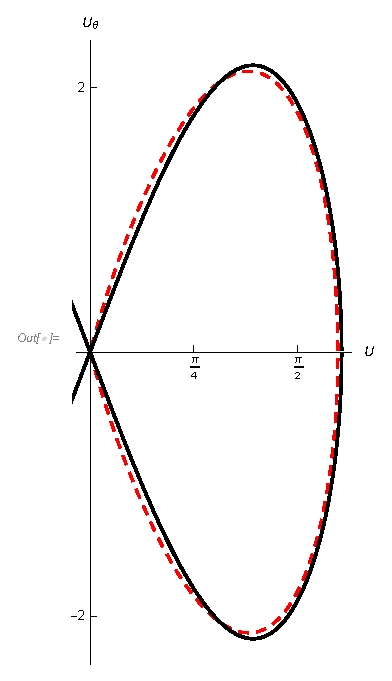
\includegraphics[width=0.75\textwidth]{images/boundary_fig1.eps}
		%\caption{Homoclinic tarjectory of the solution to Eq. (\ref{simeq4}) (solid liane) and the trajectory of target function (\ref{target}) (dashed line).}
		\caption{Гомоклиническая траектория решения уравнения (\ref{simeq4}) (сплошная линия) и траектория целевой функции (\ref{target}) (пунктирная линия).}
		\label{bound_figure1}
	\end{center}
\end{figure}
%Typical profile of the phase portrait of Eq.(\ref{simeq4}) is shown by solid line in Fig.1. However, traveling wave solutions exist under specific initial conditions. Recently the method of control of the wave localization has been developed in \cite{fradkov, porant16,  porandr17}. It was found that additional control terms in the equation can support stable propagation of nonlinear localized waves. In our case the control terms may be modeled by an external loading. Indeed,  assume that  the tangential external force in Eq. (\ref{simeq1}) is
% from the article
%Typical profile of the phase portrait of Eq. (\ref{simeq4}) is shown by solid line in Fig. 1. However, traveling wave solutions exist under specific initial conditions in the form of the wave at t = 0. Recently the method of control of the wave localization has been developed in Refs. \cite{bound_fradkov, bound_porant16,  bound_porandr17}. It was found that the additional control terms in the equation can support stable propagation of nonlinear localized waves even if the initial conditions are far from those required for the traveling wave existence without control. In our case the control terms can be modeled by an external loading on the lateral surface of the layer. Indeed, assume that the tangential external force in Eq. (\ref{simeq1}) is

Типичный профиль фазового портрета для уравнения (\ref{simeq4}) показан сплошной линией на рис. \ref{bound_figure1}. Однако решения с бегущей волной существуют при определенных начальных условиях в виде волны при t = 0. \fixme{Недавно в работах \cite{bound_fradkov, porant16, bound_porandr17} был представлен метод управления локализацией волн}. Было показано, что дополнительные управляющие члены в уравнении могут поддерживать устойчивое распространение нелинейных локализованных волн, даже если начальные условия далеки от тех, которые требуются для существования бегущей волны. В нашем случае условия управления можно смоделировать внешней нагрузкой на боковую поверхность слоя. Действительно, предположим, что касательная внешняя сила в уравнении (\ref{simeq1}) представлена в виде
\begin{equation}
	f_\tau=-\frac{k_1}{F_5}\left(q_1 F_7 U^*_x+q_2 F_{13} U^*_{xt}+q_1 F_8 u^*_x+q_2 F_{11} u^*_{xt}\right) \label{control}
\end{equation}
%where $U^*(x,t)$, $u^*(x,t)$ are the target functions. Then the r.h.s. of the first equation of motion has the form of the  control function according to the speed-gradient feedback control method \cite{fradkov, porant16,  porandr17, porant17}. Numerical sumulations reveal the stable propagation of localized waves for a particular case  Eqs. (\ref{simeq1}),  (\ref{simeq2}) \cite{porant17}. The problem is that the algorithm of control requires analytical expression for the target functions while Eqs. (\ref{simeq1}),  (\ref{simeq2}) don't have it in the general case. Then one can suggest to find the suitable expression by coinciding its homoclininv orbit with that of Eq. (\ref{simeq4}).
% from the article
%where $U^*(x,t)$, $u^*(x,t)$ are the target functions or desired waves. Then the r.h.s. of Eq. \ref{simeq1} has the form of the control function according to the speed-gradient feedback control method \cite{bound_fradkov, porant16,  bound_porandr17, porant17}. Numerical simulations reveal the stable propagation of localized waves for a particular case of Eqs. (\ref{simeq1}),  (\ref{simeq2}) at rather arbitrary initial conditions \cite{porant17}. However, the algorithm of control requires an analytical expression for the target functions. One can suggest to find the suitable expression by suiting its homoclinic orbit with that of Eq. (\ref{simeq4}).
где $U^*(x, t)$, $u^*(x, t)$ --- целевые функции или желаемые волны. Тогда правая часть уравнения \ref{simeq1} имеет вид функции управления с обратной связью согласно методу скоростного градиента \cite{bound_fradkov, porant16, bound_porandr17, porant17}. Численное моделирование показывает устойчивое распространение локализованных волн для частного случая уравнений (\ref{simeq1}), (\ref{simeq2}) при довольно произвольных начальных условиях \cite{porant17}. Однако алгоритм управления требует аналитического выражения для целевых функций. Можно найти подходящее выражение, совместив его гомоклиническую орбиту с орбитой уравнения (\ref{simeq4}). 
%In particular, the target functions in the form of a bell-shaped solitary wave can be suggested as
В частности, целевую функцию в виде уединенной волны колоколообразной формы можно предложить в виде
\begin{equation}
	u^*=\kappa_1 {\text{sech}}^4 (\kappa_2(x- c t- x_0)), \label{target}
\end{equation}
%Choosing the values of its parameters, $\kappa_i, x_0$, one can achieve the close trajectories shown  in Fig.1  by solid and dashed lines. equation (\ref{Uth}) is used to develop the target functions $U^*_x$ and $U^*_{xt}$. Obtained functions can be substituted into the control algorithm (\ref{control}) to study a tendence of an initial perturbation to a stable traveling wave defined by the target function (\ref{target}).
%Choosing the values of its parameters, $\kappa_i, x_0$, one can achieve the close trajectory shown in Fig. \ref{bound_figure1} by the solid and dashed lines. Eq. (\ref{Uth}) is used to develop the target functions $U^*_x$ and $U^*_{xt}$ using Eq. (\ref{target}). Obtained functions can be substituted into the control algorithm (\ref{control}) to study a tendency of an initial perturbation to a stable traveling wave defined by the target function (\ref{target}). This will be done elsewhere.
Перебирая значения ее параметров, $\kappa_i, x_0$, можно подобрать их таким образом, что траектории целевой функции $u^*$ и точного решения будут достаточно близки, как показано на рис. \ref{bound_figure1} штриховой и сплошной линиями соответственно. Уравнение (\ref{Uth}) используется для разработки целевых функций $U^*_x$ и $U^*_{xt} $ с использованием уравнения (\ref{target}). Полученные функции могут быть подставлены в алгоритм управления (\ref{control}) для изучения эволюции начального возмущения произвольной формы к устойчивой бегущей волне формы, определяемой целевой функцией (\ref{target}).

%\section{Weakly nonlinear case}
\section{Слабо нелинейный случай}
\fixme{Разделить на три части: преобразование уравнений, описание численной модели (?), численные результаты.}

%Consider small internal variations, $u_0 \ll 1$. In this case trigonometric nonlinearities in Eqs. (\ref{simeq1}), (\ref{simeq2}) can be expanded in power series. Only the leading order nonlinear terms are left. Also  consideration of the  long waves means that each order of derivation lowers the order of the term. The assumptions applied to  Eqs. (\ref{simeq1}), (\ref{simeq2})  give rise to the governing equations
%article
%Consider small internal variations, $u_0 \ll 1$, $U_{0,x} \ll 1$. In this case trigonometric nonlinearities in Eqs. (\ref{simeq1}), (\ref{simeq2}) can be expanded in power series. Consider only the leading order nonlinear terms without development of the formal asymptotic solution. Then Eqs. (\ref{simeq1}), (\ref{simeq2}) become
Рассмотрим \fixme{малые внутренние возмущения}, $u_0 \ll 1$, $U_{0, x} \ll 1$. В этом случае тригонометрические нелинейности в уравнениях (\ref{simeq1}), (\ref{simeq2}) могут быть разложены в степенные ряды. Оставляя при рассмотрении нелинейные члены только старшего порядка, уравнения (\ref{simeq1}), (\ref{simeq2}) преобразуются к виду
\[
\rho U_{0,tt}- F_1 U_{0,xx}- F_2 u_{0,xx}-F_{31} u_0 u_{0,x}=F_5 f_\tau+k_1 q_1 (F_7 U_{0,x}+F_8 u_{0,x})+
\]
\begin{equation}
	k_1 q_2 (F_{11} u_{0,xt}+ F_{13} U_{0,xt}) , \label{weakeq1}
\end{equation}
\begin{equation}
	(f_1+p)u_0+f_3 U_{0,xx}-s_{xx} u_0 U_{0,x}=0. \label{weakeq2}
\end{equation}
%Even the exact traveling wave solution to Eqs. (\ref{weakeq1}), (\ref{weakeq2}) is unknown. Then an approximate solution can be elaborated using the asymptotic slaving principle \cite{porpas}. According to it, Eq.(\ref{weakeq2}) can be resolved for $u_0$ using the above mentioned assumptions, and looking for a solution
Точное решение в виде бегущей волны для системы (\ref{weakeq1}), (\ref{weakeq2}) также неизвестно. Тем не менее, приближенное решение может быть получено с использованием \fixme{принципа асимптотического подчинения} \cite{bound_porpas}. Согласно этому принципу, уравнение (\ref{weakeq2}) может быть решено относительно $u_0$, используя вышеупомянутые предположения в виде
\[
u_0=u_{01}+u_{02}+u_{03}...
\]
%where
% from the article
%where $u_{03} \ll u_{02} \ll u_{03}$. Also consideration of the long waves means that each order of derivation lowers the order ofthe term, e.g. $U_{0,xx} \ll U_{0,x}$. This allows us to separate the terms in the weakly nonlinear Eq. \ref{weakeq2} by orders,
где $u_{03} \ll u_{02} \ll u_{03}$ и т.д.. Рассмотрение длинных волн также означает, \fixme{что каждая производная понижает порядок члена}, например $ U_{0, xx} \ll U_{0, x} $. Это позволяет разделить члены в слабонелинейном уравнении \ref{weakeq2} по степеням,
\[
\left((f_1+p) u_{01} + f_3 U_{0,xx}\right) + \left((f_1+p) u_{02} - s_{xx} u_{01} U_{0,x}\right) + \cdots = 0.
\]
%Then one approximately obtains
% Equating to zero the terms in big brackets separately one obtains the solutions for $u_{0i}$
Обнуляя слагаемые в больших скобках по отдельности, получаем решения для $u_{0i}$
\[
u_{01} = -\frac{f_3 U_{0, xx}}{f_1+p}, u_{02}= \frac{f_3 s_{xx} U_{0,x}U_{0,xx}}{(f_1+p)^2}.
\]
Таким образом, приближенное решение имеет вид
\begin{equation}
	u_0=-\frac{f_3 U_{0,xx}}{f_1+p}+\frac{f_3 s_{xx} U_{0,x} U_{0,xx}}{(f_1+p)^2}\label{weakeq3}.
\end{equation}
%Substitution of Eq. (\ref{weakeq3}) into Eq. (\ref{weakeq1}) results in an equation for $U_0$,
Подставляя (\ref{weakeq3}) в уравнение (\ref{weakeq1}) получаем уравнение для $U_0$,
\[
\rho U_{0,tt}- F_1 U_{0,xx}+ \frac{f_3 F_2}{f_1+p}U_{0,xxxx}+\frac{f_3 s_{xx} F_{2}}{2(f_1+p)^2} (U_{0,x}^2)_{xxx}+
-\frac{f_3^2 F_{31}}{2(f_1+p)^2} (U_{0,xx}^2)_{x}=
\]
\begin{equation}
	F_5 f_\tau+k_1 q_1 F_7 U_{0,x} + k_1 q_2 F_{11}U _{0,xt}\label{weakeq4}
\end{equation}

%The last equation doesn't have even exact traveling wave solution in the absence of an external loading, $f_\tau = 0, k_1 = 0$. Shown in Fig. \ref{bound_figure2} is the  evolution of an initial bell-shaped perturbation,
\begin{figure}
	\begin{center}
		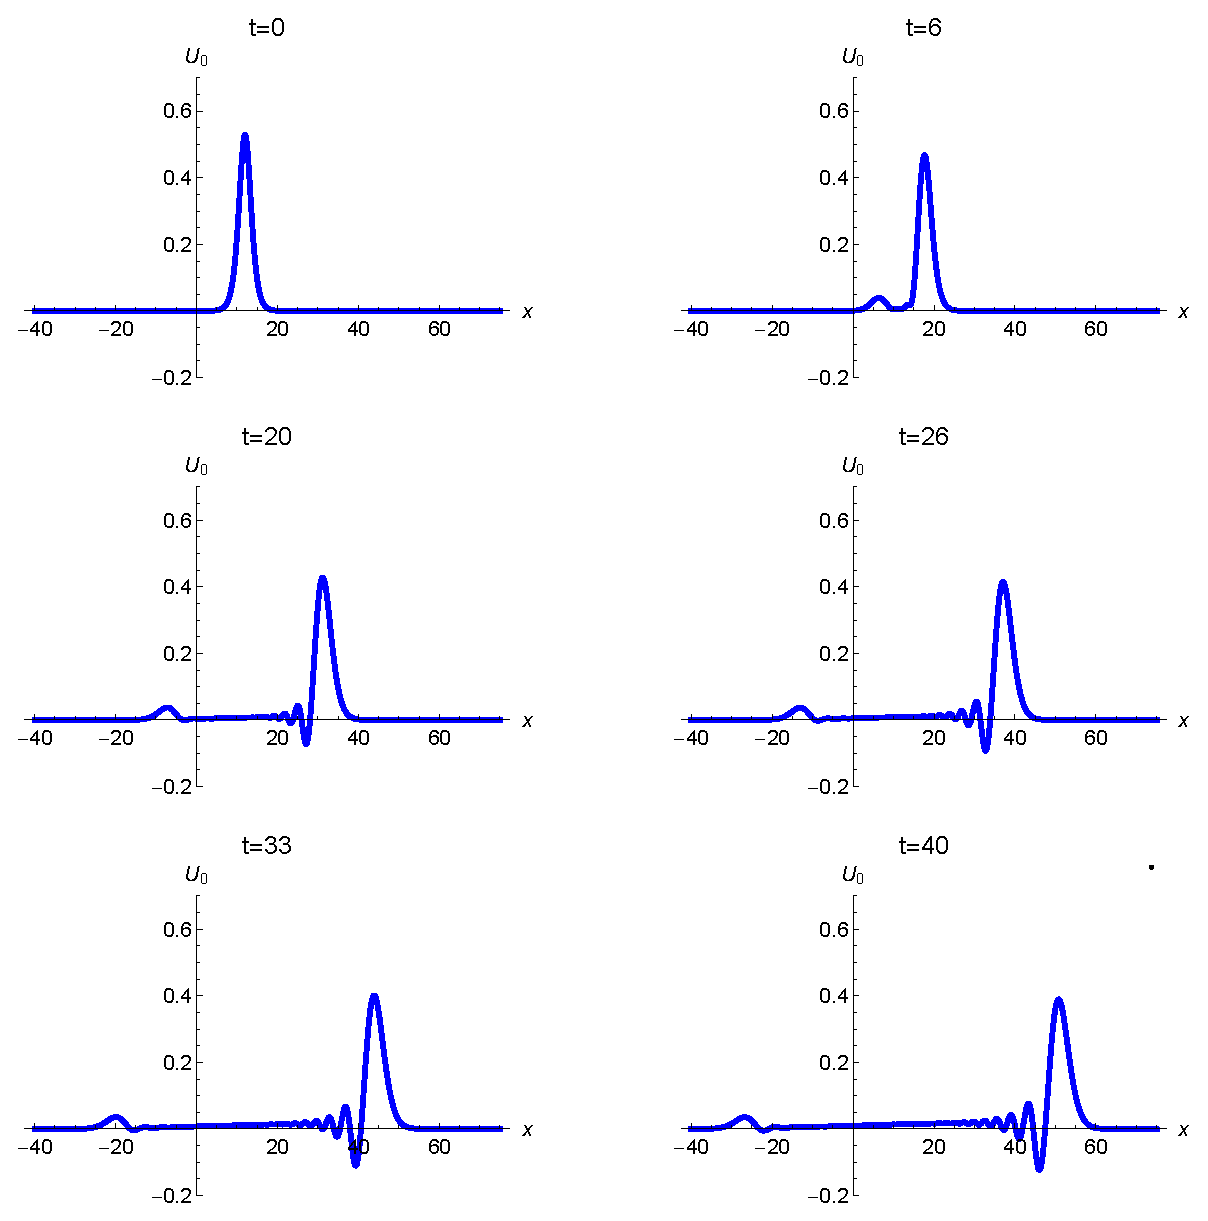
\includegraphics[width=0.95\textwidth]{images/boundary_fig2.eps}
		%\caption{Evolution of the bell-shaped input in the weakly nonlinear case  without external loading.}
		\caption{Эволюция колоколообразного начального возмущения в слабонелинейном случае без внешней нагрузки.}
		\label{bound_figure2}
	\end{center}
\end{figure} 
Последнее уравнение все еще не имеет точного решения в виде уединенной бегущей волны при отсутствии внешней нагрузки, $f_\tau = 0, k_1 = 0$. На рисунке \ref{bound_figure2} показана эволюция решения при начальном условии в виде колоколообразного возмущения следующего вида,
%\begin{equation}
$$
	U_0^*(x,0)=s_1 {\text{sech}}^2 (k (x-x_0)),
$$
$$	
	U_{0,t}^*(x,0)= s_2 {\text{sech}}^2 (k (x-x_0)) {\text{tanh}} (k (x-x_0)). %\label{target}
$$
%\end{equation}
%Here s1, s2, x0 are the constant parameters. One can see that the initial profile of U0 is not kept: the oscillations behind the wave arise, and an extra hump is developing. The former factor is caused by dispersion term U0,xxxx while the latter one appears due to nonlinear term (U20,x)xxx.
Здесь $s_1$, $s_2$, $x_0$ --- постоянные параметры. На рисунке видно, что исходный профиль $U_0$ не сохраняется в ходе эволюции: за волной возникают колебания и появляется лишний горб. Первый фактор вызван дисперсионным членом $U_{0, xxxx}$, а второй --- нелинейным членом $(U_{0, x}^2)_{xxx}$.
\begin{figure}[h]
	\begin{center}
		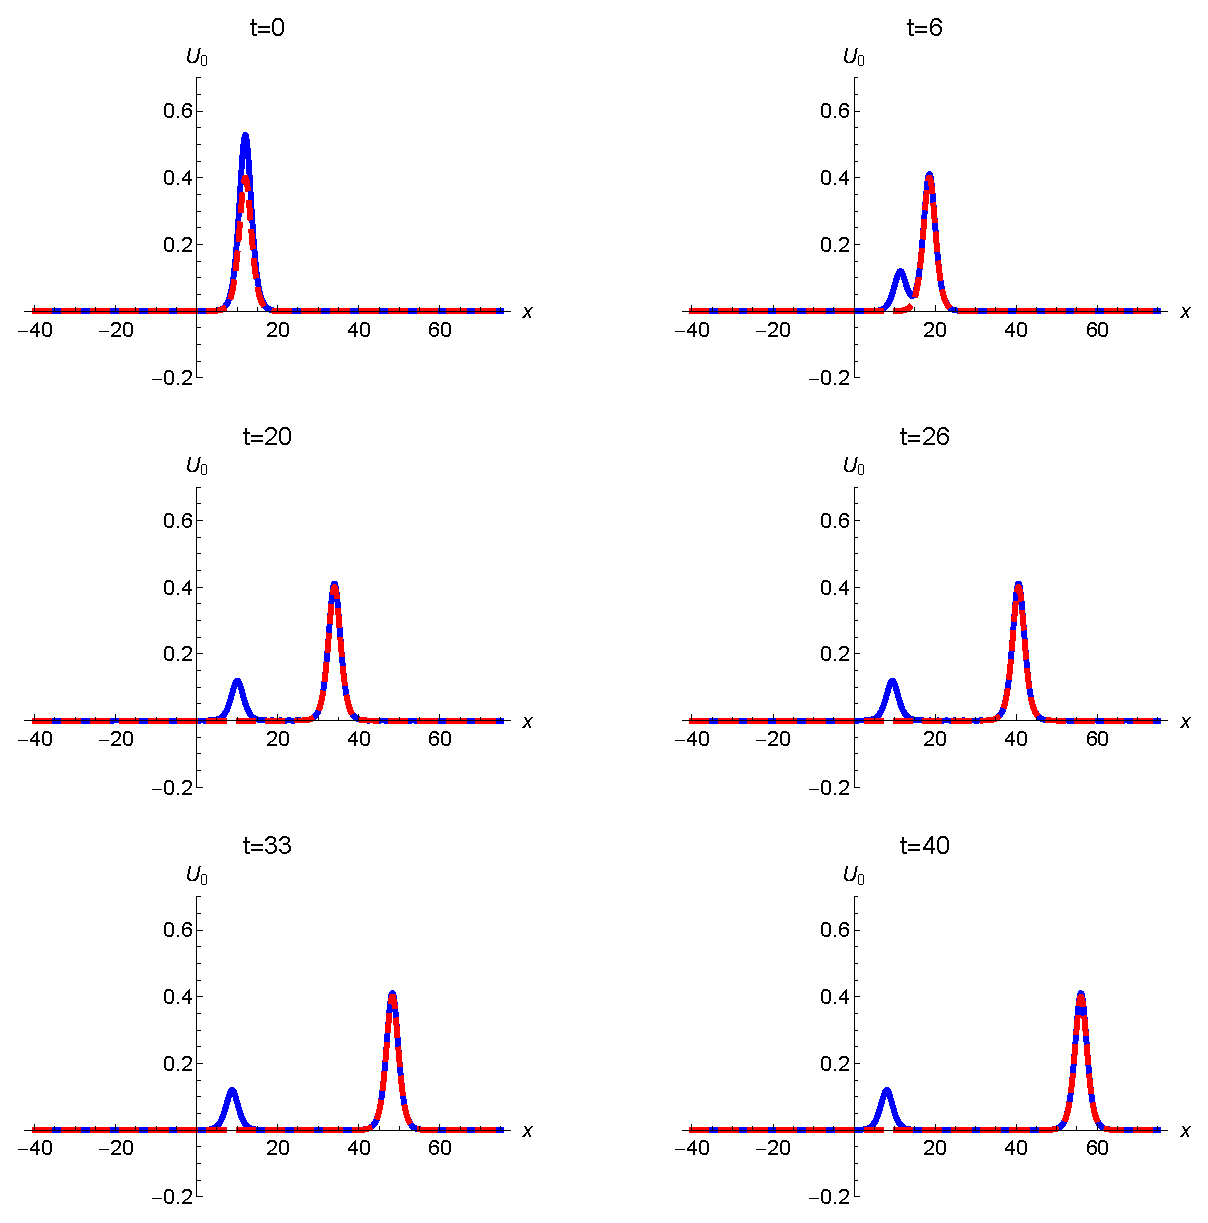
\includegraphics[width=0.95\textwidth]{images/boundary_fig3.eps}
		%\caption{Evolution of the bell-shaped input in the weakly nonlinear case  thanks to the external loading. Shown by dahsed line is the target function $U_0^*$.}
		\caption{Эволюция колоколообразного начального возмущения в слабонелинейном случае при наличии внешней нагрузки. Пунктирной линией показана целевая функция $U_0^*$.}
		\label{bound_figure3}
	\end{center}
\end{figure}
%In the absence of an external loading, $f_\tau=0$, $k_1=0$.  Here $s_1$, $s_2$, $x_0$ are the constant parameters. One can see that the  initial profile of $U_0$ is not kept: oscillations behind the wave arise, and an extra hump is developing. The former factor is caused by dispersion term $U_{0,xxxx}$ while the latter one appears due to the nonlinear term $(U_{0,x}^2)_{xxx}$. This may be checked considering particular cases with the absence of nonlinearity and the presence of only one nonlinear term.

%The presnce of an external loading changes the wave evolution as shown in Fig.3. It is assumed to consider the external force $f_\tau$ in the form
Наличие внешней управляющей нагрузки изменяет эволюцию волны, как показано на рисунке \ref{bound_figure3}. Предлагается рассматривать внешнюю силу $f_\tau$ в виде
\[
f_\tau=-\frac{k_1}{F_5}\left(q_1 F_7 U^*_{0,x}(x,t)+  q_2 F_{11} U_{0,xt}^*(x,t)\right),
\]
%where
где
\[
U^*_0(x,t)=s_1 {\text{sech}}^2 (k (x-w t-x_0)),
\]
%$w$ is a constant velocity. One can see that the r.h.s. in Eq. (\ref{weakeq4}) becomes of the form of the control function according to the speed gradient method \cite{horizont, porant16, porant17}. Temporal evolution of the function $U_0$ in Fig. 3 demonstrates fast tendency to the target function $U_0^*$ shown by dashed line. Then the stable propagation of the bell-shaped wave is observed.
%$w$ is a constant velocity. One can see that the r.h.s. in Eq. (\ref{weakeq4}) becomes of the form of the control function according to the speed gradient method \cite{horizont, porant16, porant17}. Temporal evolution of the function $U_0$ in Fig. 3 demonstrates fast tendency of the hump moving to the right to the target function $U_0^*$. We have added the target function by the dashed line in Fig. \ref{bound_figure3}, however, it is practically invisible there due to the closeness to the solid line profile of the numerical solution Then the stable propagation of the bell-shaped wave is observed.
$w$ --- постоянная скорость. Видно, что правая часть уравнения (\ref{weakeq4}) является по сути управляющей функцией согласно методу скоростного градиента \cite{bound_horizont, porant16, porant17}. Временная эволюция  $U_0$ на рис. \ref{bound_figure3} демонстрирует быструю тенденцию смещения горба вправо к целевой функции $U_0^*$. Целевая функция изображена пунктирной линией, однако она там практически не видна из-за близости к профилю численного решения. После достижения профиля волны целевой функции наблюдается устойчивое распространение колоколообразной волны, поддерживаемое управляющей нагрузкой. \fixme{Добавить описание к паразитному эффекту в виде малой медленной колоколообразной волны за профилем основной}.

\section{Заключение}
%The nonlinear strain waves may propagate in a layer made of material having a di-atomic crystalline structure. The modeling is based on the continuum approach using the expressions for the strain energy previously obtained as a continuum limit of the discrete di-atomic crystalline lattice problem. The asymptotic procedure is developed to transform an initial two-dimensional problem to a solution of  one-dimensional governing equations. In general, it is described by the coupled nonlinear equations for macro-displacements and variations in an internal structure.  The expressions for the coefficients in the equations are obtained in terms of the parameters of the original two-dimensional di-atomic lattice. The weakly nonlinear case allows us to employ a slaving principle and reduce the solution of the coupled equation to the solution of a single nonlinear equation for the macro-displacements.
%The nonlinear strain waves may propagate in a layer made of a material having a di-atomic crystalline structure. The modeling is based on the continuum approach using the expressions for the strain energy previously obtained as a continuum limit of the discrete di-atomic crystalline lattice problem. The asymptotic procedure is developed to transform the solution to the initial two-dimensional problem to the solution of the one-dimensional coupled nonlinear equations for macro-displacements and variations in an internal structure. The expressions for the coefficients in the equations are obtained in terms of the parameters of the original two-dimensional di-atomic lattice. The weakly nonlinear case allows us to employ a slaving principle and reduce the solution of the coupled equations to the solution of a single nonlinear equation for the macro-displacements.
\fixme{Исправить}

Нелинейные волны деформации могут распространяться в слое из материала, имеющего двухатомную кристаллическую структуру. Моделирование основано на континуальном подходе с использованием выражений для энергии деформации, ранее полученных в качестве континуального предела дискретной задачи двухатомной кристаллической решетки. Разработана асимптотическая процедура преобразования решения исходной двумерной задачи в решение одномерных связанных нелинейных уравнений для макроперемещений и вариаций внутренней структуры. Выражения для коэффициентов в уравнениях получены через параметры исходной двумерной двухатомной решетки. Слабо нелинейный случай позволяет использовать принцип подчинения и свести решение связанных уравнений к решению одного нелинейного уравнения для макроперемещений.

%However, the main result concerns mechanical realization of the feedback control algorithm previously formally developed in Refs. \cite{bound_horizont,bound_fradkov, porant16,  bound_porandr17, porant17}. It is shown that  an external loading acting on a lateral surface of a layer can realize the control algorithm. It allows us to support stable bell-shaped solitary wave propagation like it is seen in Fig.3. Of course, other target functions may be used instead of Eq. (\ref{target}). This was demonstrated for various nonlinear equations in our previous works \cite{porant16, bound_porandr17, porant17}.
Однако основной результат касается механической реализации алгоритма управления с обратной связью, ранее формально разработанного в \cite{bound_horizont, bound_fradkov, porant16, bound_porandr17, porant17}. Показано, что внешняя нагрузка, действующая на боковую поверхность слоя, позволяет реализовать алгоритм управления. Это позволяет поддерживать устойчивое распространение уединенной волны колоколообразной формы, как показано на рисунке \ref{bound_figure3}. Конечно, вместо уравнения можно использовать другие целевые функции (\ref{target}). Это было продемонстрировано для различных нелинейных уравнений в наших предыдущих работах \cite{porant16, bound_porandr17, porant17}.           % Глава 1
\chapter{On control of harmonic waves in  an acoustic metamaterial}

Generation of harmonic waves in a mass-in mass model of an acoustic metamaterial is considered. It is shown numerically that outside the band gap, the boundary harmonic excitation gives rise to a formation of periodic waves whose profile gradually coincides with the profile of the exact travelling wave harmonic solution. No waves are generated by the boundary excitation inside the band gap. A switch-on/off control is developed to achieve the formation of the harmonic waves inside the band gap.
  
\section{Introduction}

The interest to the study of the acoustic metamaterials has grown considerably in the recent years, see \cite{Cummer,Cvet, Huang2010, Ma, muller, delis1, Eremeyev2020, Porubov2019, Erofeev2020} and references therein. The linear acoustic metamaterials draw  more attention \cite{Cvet, Huang2010,  muller}. One of the simplest but instructive model is the mas-in-mass model. It allows to describe the band gap in the dispersion relation \cite{Cvet, Huang2010}, negative effective mass  and other features related to a metamaterial. 

Experimental realization of the mass-in-mass  model may be found in \cite{Cvet,Yang, Yao2008, Zhou2015}. The existence of band gap was confirmed there. However, no periodic waves were recorded. The metamaterial has been constructed in \cite{Yang} so as to change the internal oscillator by an electric signal. Similarly the 
 external electromagnetic signals were used in \cite{Chen2014,Xiao2015} to develop the active tunable acoustic metamaterials. One can note the luck of theoretical results concerning generation of the harmonic waves and their control.

In this paper we study numerically generation  of harmonic waves in  a linear metamaterial mass-in-mass model.  The boundary harmonic excitation is shown to produce both the acoustic and optic harmonic waves outside the band gap while no wave propagation is obtained inside the bamd gap. Then the switch-on/off control is developed to see how to change the shape of the harmonic waves inside and outside the band gap.

\section{Statement of  problem}

Consider a  chain   when interaction between the  masses,  $m$,  is modeled by linearly- elastic springs \cite{Huang2010}. An elastic internal oscillator is modelled by the additional masses $m_1$ , attached by springs to each mass $m$ in the chain, and this interaction is also linear and elastic. Masses $m_1$ do not interact directly between themselves. The displacement of the mass $m$ with the number $n$ is denoted by $x_n$, while that of $m_1$ is denoted by $y_n$.

\begin{equation}
\ddot{x_n}=\beta_0 (x_{n-1}-2x_n+x_{n+1})+\eta \beta_1 (y_n-x_n), 
\label{eq1}
\end{equation}
\begin{equation}
\ddot{y_n}=-\beta_1 (y_n-x_n). \label{eq2}
\end{equation}
Here $\eta=m_1/m$, while the linear stiffness of the spring of the chain is $\beta_0 m$,  the nonlinear stiffness is $\beta_3 m$. Corresponding linear and nonlinear stiffnesses of the attached spring are $\beta_1 m_1$ , $\beta_2 m_1$ respectively. 
\begin{figure*}[h]
\begin{center}
%\begin{flushleft}
%\end{flushleft}
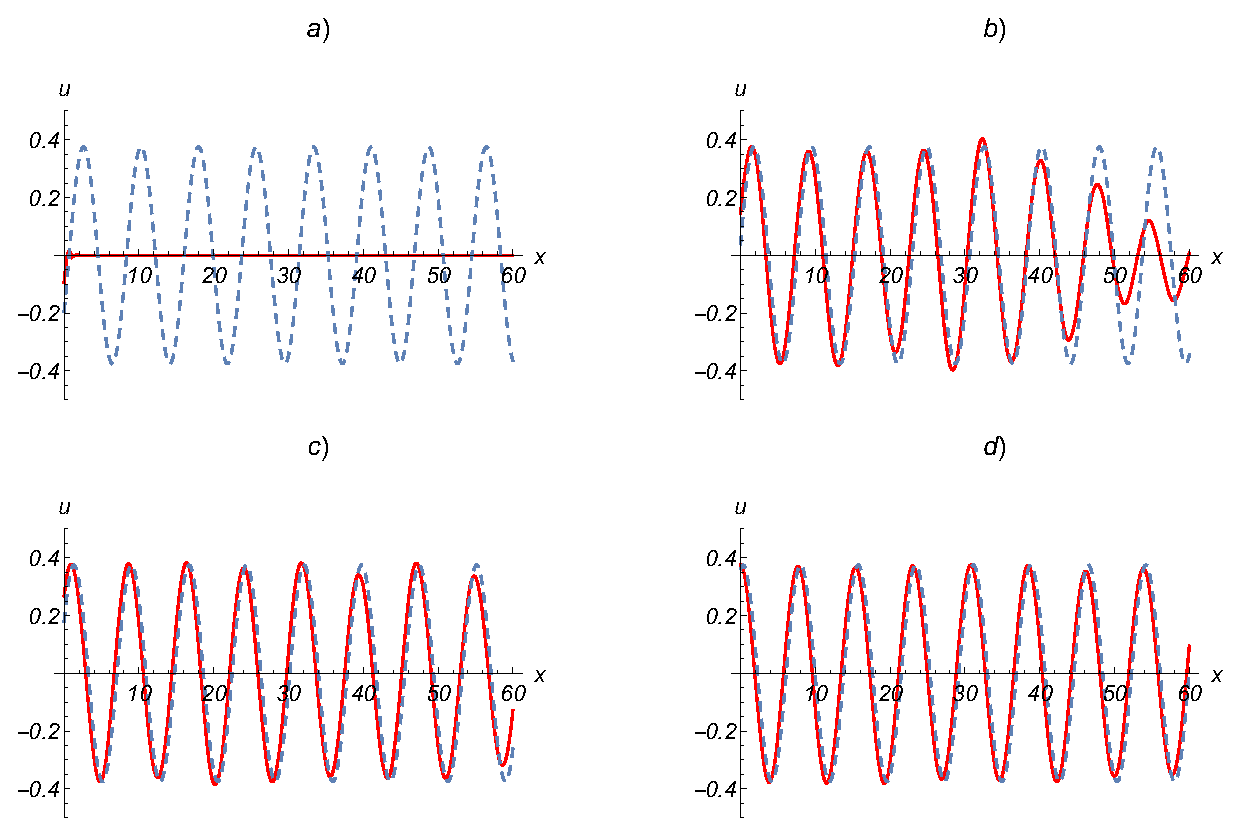
\includegraphics[scale=.5]{new_pic/fig1.eps}
\end{center}
\caption{ Evolution of $u$ wave below the band gap, $\omega<\sqrt{\beta_1}$. Shown by dashed line is the imagine part of the  exact solution (\ref{solfin}) with the frequency $\omega=\omega_a$.  a)$t=0$; b)$ t=t_N/4$; c) $t=t_N/2$, d)$t=t_N$.}
\label{fg1}
  \end{figure*}
We proceed with a continuum limit of Eqs. (\ref{eq1}), (\ref{eq2}). Following the standard procedure we introduce the continuum functions $u(x,t)$, $v(x,t)$ for description of the displacements of the masses $m$, $m_1$ with the number $n$ while the continuum displacements of the neighboring masses are sought using the Taylor series around $u$. Retaining only the first nonzero term in the expansion we obtain
\begin{equation}
u_{tt}=\beta_0 h^2 u_{xx}+\eta \beta_1 (v-u), \label{eq3}
\end{equation}
\begin{equation}
v_{tt}=-\beta_1 (v-u), \label{eq4}
\end{equation}
where $h$ is a distance between the masses $m$ in the chain. 
The conventional traveling wave solution is sought as 
\begin{equation}\label{sol}
 u=A\exp (\imath(p~ x - \omega~ t- p~ x_0)), ~
   v=B \exp (\imath(p~ x - \omega~ t-p~ x_0))
\end{equation}
Substituting Eq. (\ref{sol}) into Eqs. (\ref{eq3}), (\ref{eq4}) one obtains the known dispersion relation \cite{Huang2010} 
\[
\omega^4 -(\beta_1(1+\eta)+\beta_0 p^2 h^2)\omega^2+\beta_0 \beta_1 p^2 h^2=0.
\]
whose solution is 
\begin{equation}\label{acdiscr}
\omega_a^2=\frac{\beta_1(1+\eta)+\beta_0 h^2 p^2}{2}-\frac{\sqrt{D}}{2},
\end{equation}
\begin{equation}\label{optdiscr}
\omega_o^2=\frac{\beta_1(1+\eta)+\beta_0 h^2 p^2}{2}+\frac{\sqrt{D}}{2},
\end{equation}
where
\[
D=(\beta_1(1+\eta)+\beta_0 h^2 p^2)^2-4\beta_0 h^2 p^2,
\]

Also the expression for $A$ through  $B$ is obtained giving rise to the solution for $u$ and $v$ in the final form
\begin{equation}\label{solfin}
 u=\frac{\beta_1-\omega^2}{\beta_1}~B\exp (\imath(p~ x - \omega~ t- p~ x_0)), ~
   v=B \exp (\imath(p~ x - \omega~ t- p~ x_0)),
\end{equation}
where the frequency is  $\omega=\omega_a$,  or $\omega=\omega_o$, $x_0$ accounts for an initial phase.
The acoustic band frequency varies from $0$ to $\sqrt{\beta_1}$\, while the optic one lies in the interval 
$(\sqrt{\beta_1(1+\eta)}, \infty)$. Therefore, there is a band gap $\sqrt{\beta_1}<\omega<\sqrt{\beta_1(1+\eta)}$ where no harmonic traveling wave propagates.

\section{Generation of harmonic waves}
The analysis in the previous Section is based on the particular traveling wave solution which requires specific initial and boundary conditions for its realization. However, experimental generation of the waves in a metamaterial uses the boundary excitation of the waves. In particular, the following  initial and boundary conditions for $u$ can be employed,
\begin{equation}\label{bcu}
u(0,t)=\frac{\beta_1-\omega^2}{\beta_1}~B~ {\rm sin} (\omega ~t),~u(x,0)=0, ~u(x,0)_t=0,
\end{equation}
while for $v$ we assume that
\begin{equation}\label{bcv}
v(0,t)=B ~{\rm sin} (\omega ~t),~v(x,0)=0, ~v(x,0)_t=0,
\end{equation}
This problem can be solved numerically. The Wolfram Mathematica NDSolve command is used to solve Eqs. (\ref{eq3}), (\ref{eq4} with the conditions (\ref{bcu}), (\ref{bcv}). 
%The interval of calculations is $0<x<x_N$,
The interval of interest is $0<x<x_N$, 
 the absorbing boundary conditions %for $u$, $v$ 
are imposed at $x=x_N$%.
 using the following masking technique. The calculation domain $0 < x < 3 x_N$ is being splitted into two parts:  $0 < x < x_N$ and  $x_N < x < 3 x_N$ while the system of Eq.  (\ref{eq1}), (\ref{eq2}) is replaced with
$$
U_{t}=\beta_0 h^2 u_{xx}+\eta \beta_1 (v-u)
$$
$$
u_{t}=U + u f_{\text{mask}},
$$
$$
v_{tt}=-\beta_1 (v-u),
$$
where $f_{\text{mask}} = \log \left(\tanh{0.03 (3 x_N - x)}\right)^2$. By this way, as far as $f_{\text{mask}}$ is effectievely zero in the interval of interest the exact system of Eq.  (\ref{eq1}), (\ref{eq2}) is being solved there. While for the rest part of the domain $f_{\text{mask}}$ is negative and decreasing with $x$,4 which leads to the corresponding decrease of the amplitude of the each wave frequency traveling through. The resulting amplitude of wave at $x = 3 x_N$ becames numerically very close to zero leading to nothing be reflected to the interval of interest from the $x = 3 x_N$ boundary.
\begin{figure*}
\begin{center}
%\begin{flushleft}
%\end{flushleft}
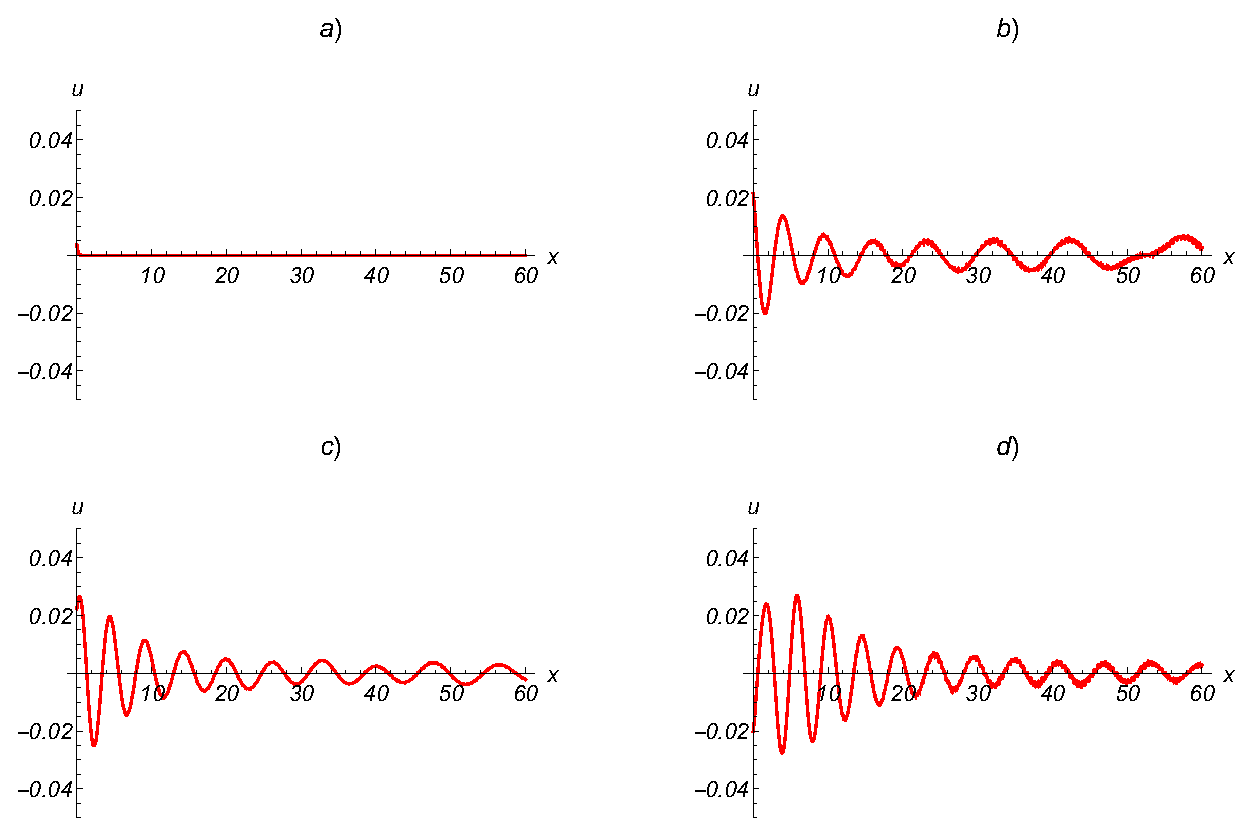
\includegraphics[scale=.45]{new_pic/fig2.eps}
\end{center}
\caption{ Evolution of $u$ wave at the lower boundary of the band gap, $\omega \approx \sqrt{\beta_1}$,  $\omega=0.3$.  a)$t=0$; b)$ t=t_N/4$; c) $t=t_N/2$, d)$t=t_N$.}
\label{fg2}
  \end{figure*}



  
The aim of calculations is to see how the harmonic boundary excitation gives rise to the harmonic wave  in time.  The imaginary parts of the solutions (\ref{solfin}) will be compared with the numerical results. For this purpose the initial position $x_0$  in Eqs. (\ref{solfin}) will be chosen so as to coincide as close as possible the numerical and analytical curves at the final time of calculations, $t=t_N$. Then both curves are placed together for the preceding moments of times. Also, the realization of the band gap will be studied by varying the frequency $\omega$ ib the boundary conditions (\ref{bcu}), (\ref{bcv}) from zero through the band gap. Therefore the values of frequency $\omega$ is defined while the wave number of the exact solution, $p$, is calculated through it using the dispersion relation,
\[
p=\omega\sqrt{\frac{\beta_1(1+\eta)-\omega^2}{\beta_0 h^2(\beta_1-\omega^2)}}.
\]
The values of the coefficients are chosen as 
$t_N = 600; x_N = 60;\beta_0=1, h = 0.5; \beta_1 = 0.1; \eta = 0.5;  B=0.25$. Then the band gap is $0.316<\omega<0.387$.

  
Shown in Fig \ref{fg1} is the formation of harmonic wave $u$ at various times when the excitation frequency lies below the band gap, $\omega<\sqrt{\beta_1}$, $\omega=0.2$, $x_0= 15.8$. The exact solution is placed on each time sketch a)-d).  One can see that initially undisturbed stage a) transforms to a non-harmonic wave which partially coincides with the harmonic exact traveling wave solution at the stage b). The last two stages c) and d) demonstrate almost full similarity between numerical and analytical solution.
\begin{figure*}
\begin{center}
%\begin{flushleft}
%\end{flushleft}
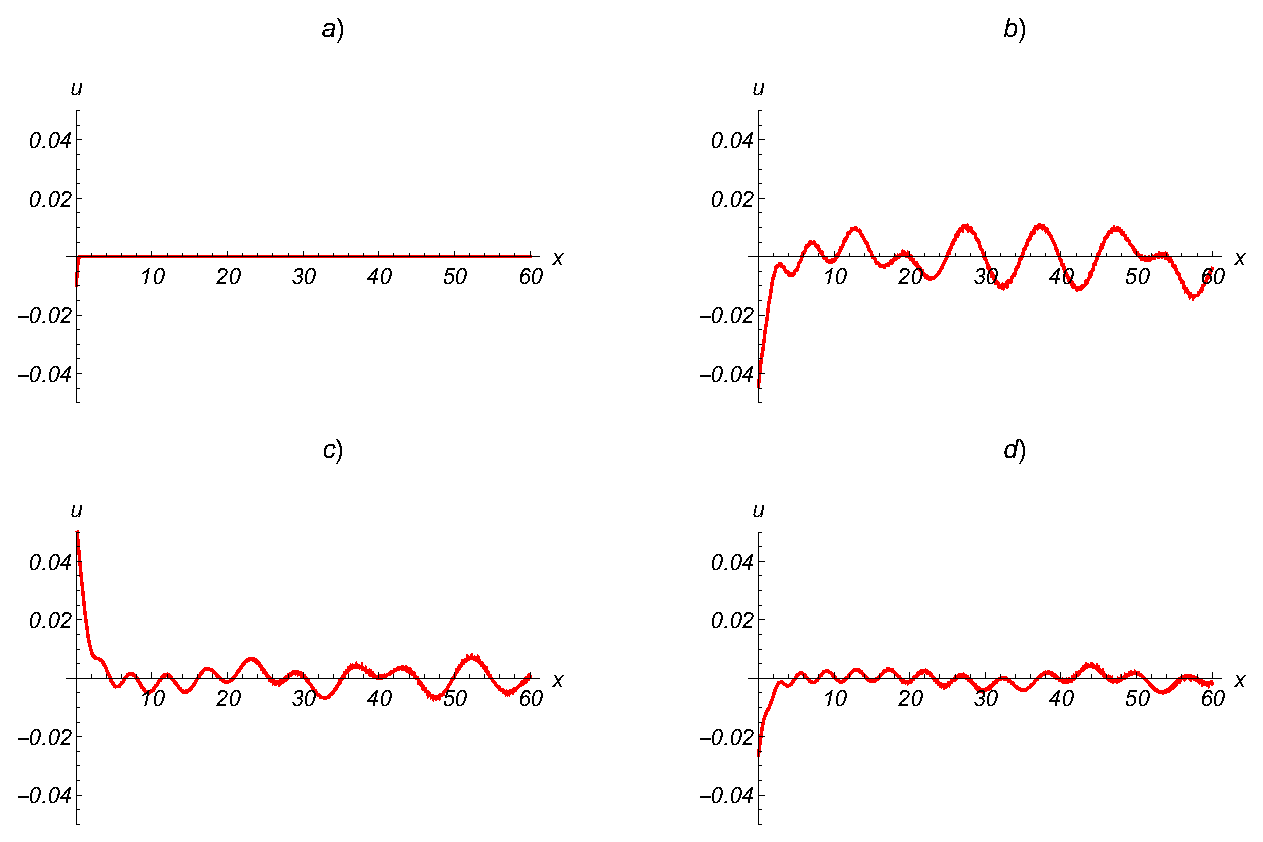
\includegraphics[scale=.45]{new_pic/fig3.eps}
\end{center}
\caption{Supression  of $u$ wave inside the band gap, $\sqrt{\beta_1}<\omega<\sqrt{\beta_1(1+\eta)}$, $\omega=0.35$. a)$t=0$; b)$ t=t_N/4$; c) $t=t_N/2$, d)$t=t_N$.}
\label{fg3}
  \end{figure*}
  
An increase in the excitation frequency up to  the lower boundary of the band gap, $\omega \approx \sqrt{\beta_1}$,  $\omega=0.3$,  results in the formation of the wave shown in Fig. \ref{fg2}. One can see no harmonic wave generation, the amplitude of the wave decays away from the left boundary. The last two stages c) and d) demonstrate almost stable wave dynamics.
\begin{figure*}
\begin{center}
%\begin{flushleft}
%\end{flushleft}
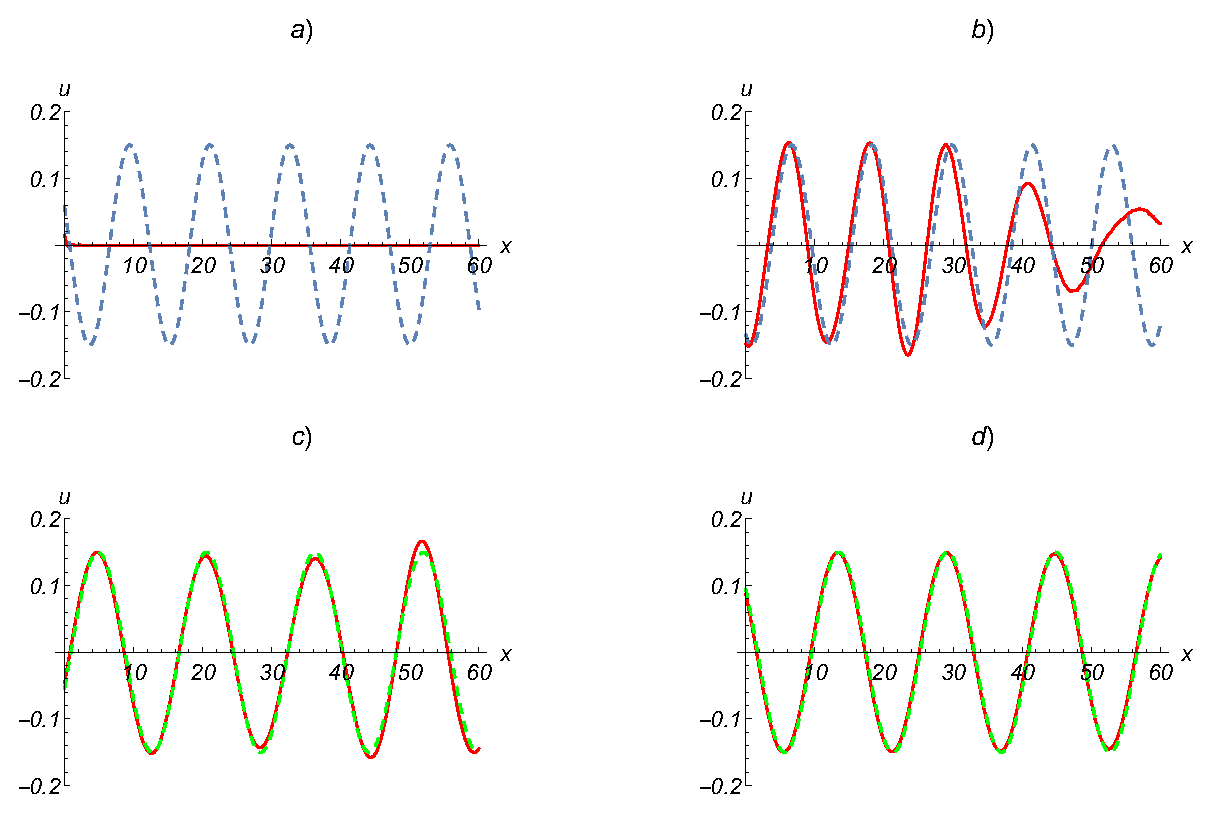
\includegraphics[scale=.45]{new_pic/fig4.eps}
\end{center}
\caption{ Control of evolution of $u$ wave below the band gap, $\omega<\sqrt{\beta_1}$ when the control switches-on at $t=t_N/4$.   a)$t=0$; b)$ t=t_N/4$. Shown by dashed line is the imagine part of the  exact solution (\ref{solfin}) ; c) $t=t_N/2$, d)$t=t_N$. Shown by dashed line is the imagine part of the  exact solution (\ref{solwave}) }
\label{fg4}
  \end{figure*}
\begin{figure*}
\begin{center}
%\begin{flushleft}
%\end{flushleft}
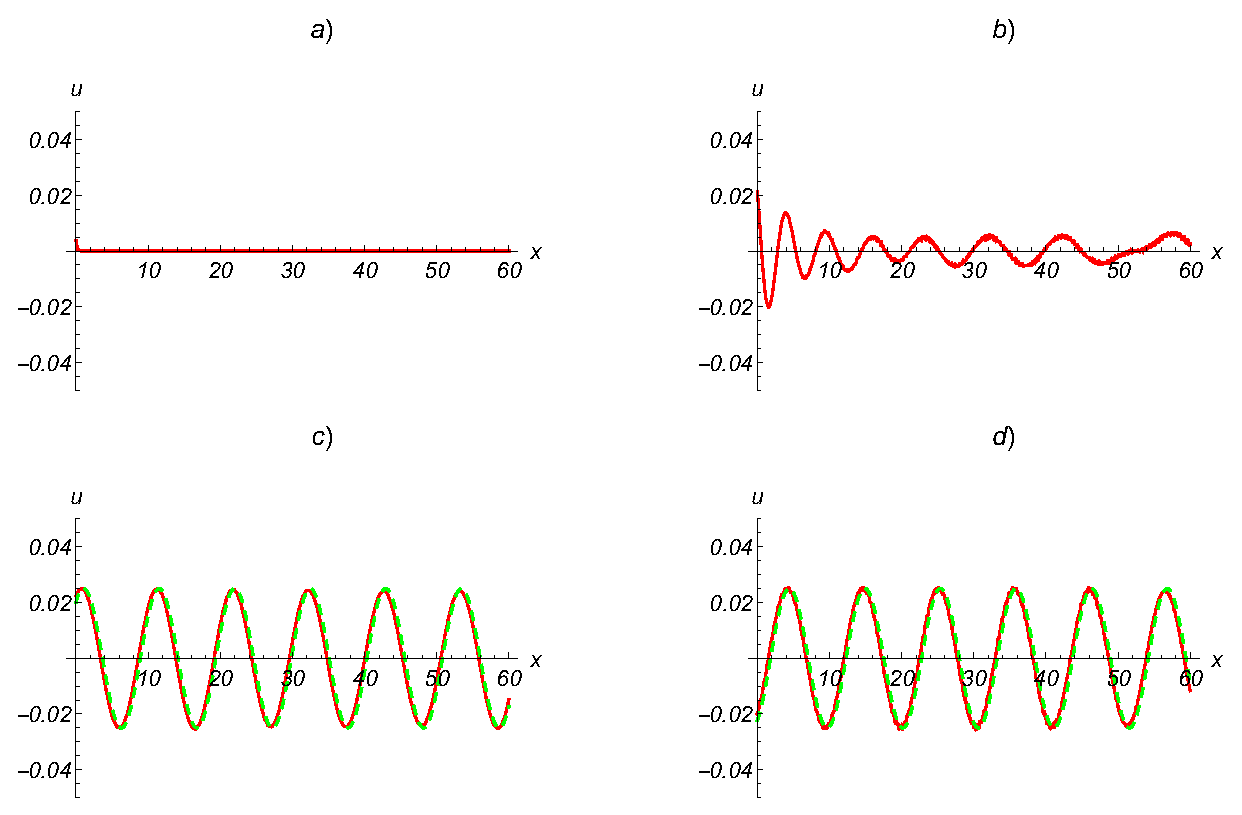
\includegraphics[scale=.45]{new_pic/fig5.eps}
\end{center}
\caption{Control of evolution of $u$ wave at the lower boundary of  the band gap, $\omega \approx \sqrt{\beta_1}$, $\omega=0.3$,  when the control switches-on at $t=t_N/4$.   a)$t=0$; b)$ t=t_N/4$ ; c) $t=t_N/2$; d)$t=t_N$. Shown by dashed line in the last two stages  is the imagine part of the  exact solution (\ref{solwave}) .}
\label{fg5}
  \end{figure*}
  
  \begin{figure*}[ht]
\begin{center}
%\begin{flushleft}
%\end{flushleft}
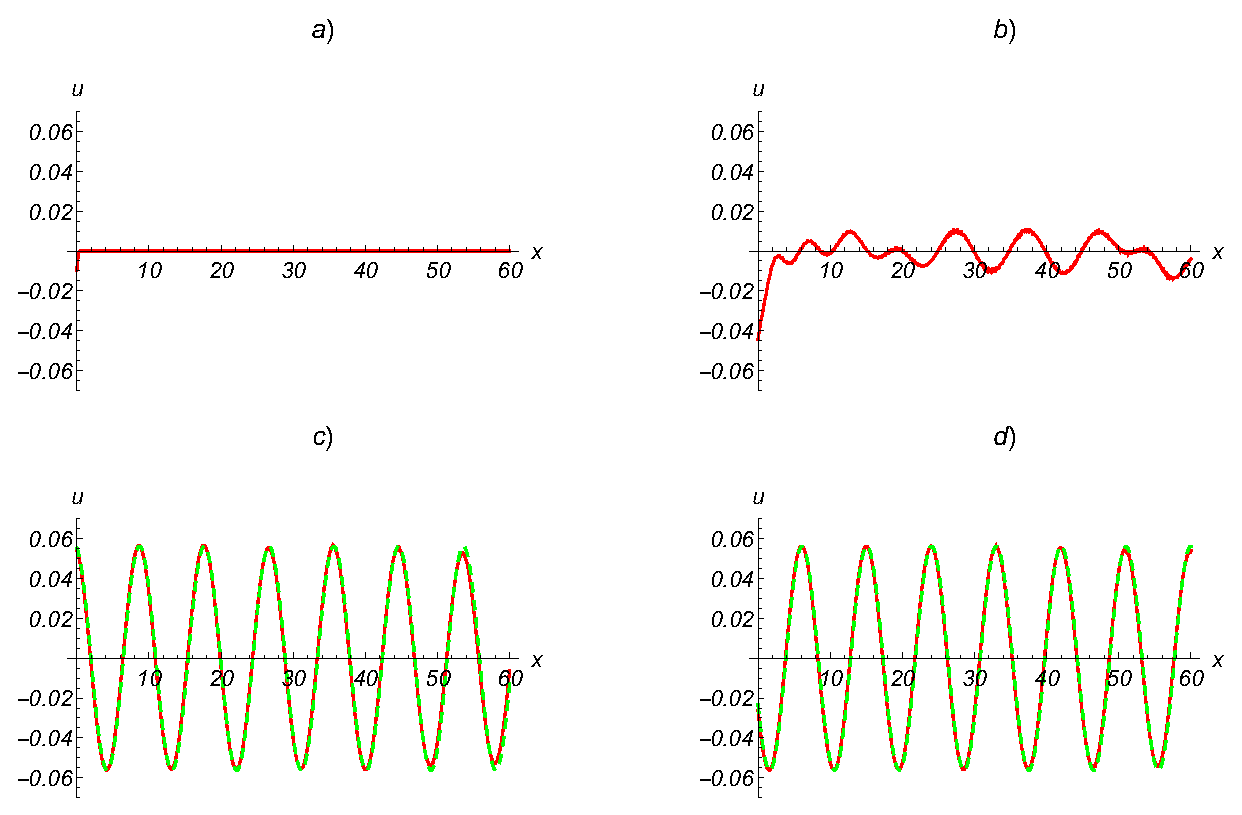
\includegraphics[scale=.45]{new_pic/fig6.eps}
\end{center}
\caption{Control of evolution of $u$ wave inside  the band gap, $\omega=0.35$,  when the control switches-on at $t=t_N/4$.   a)$t=0$; b)$ t=t_N/4$ ; c) $t=t_N/2$; d)$t=t_N$. Shown by dashed line in the last two stages  is the imagine part of the  exact solution (\ref{solwave}) .}
\label{fg6}
  \end{figure*}
Inside the band gap, $\sqrt{\beta_1}<\omega<\sqrt{\beta_1(1+\eta)}$,  $\omega=0.35$ there is no even a wave with decreasing amplitude. Shown in Fig.\ref{fg3} is a stromg decrease in the amplitude of disturbances and their chaotic character. This is in an agreement with the analysis from the previous Section.



Further increase in the value of the excitation frequency results in the realization of the dynamics shown in Fig. \ref{fg2} when the frequency achieves the value of the upper boundary of band gap. At higher frequencies a formation of periodic wave happens with the frequency belonging to the optic branch, $\omega=\omega_o$. Again the similarity with the exact solution is observed like that shown in Fig.\ref{fg1}.


  
\section{Control of harmonic waves}

The use of electromegnetic signals  in \cite{Yang,Chen2014,Xiao2015} to change the internal properties of a metamaterial suggests the mechanism of a control based on an instant switch-on. It is modelled by the unit step function $H(t_0-t)$ that switches-off  the coupling in Eqs.  (\ref{eq3}), (\ref{eq4}) at$t=t_0$. Thus, for $u$ we have

\[
u_{tt}=\beta_0 h^2 u_{xx}+\eta \beta_1 (v-u)~H(t_0-t)
\]
Also, the unit step function should be added in equation of motion  (\ref{eq4}) and  boundary condition for $v$ (\ref{bcv}). The switch-on time for the control , $t_0$, is chosen equal to $t_N/4$, other parameters of calculations are the same as in the previous Section.

Again the comparison with the exact solution will be given.  However, after switch-on the control, equation of motion for $u$ becomes the linear wave equation whose solution is 
\begin{equation}\label{solwave}
 u_w=\frac{\beta_1-\omega^2}{\beta_1}~B~{\rm sin}  (\imath(\omega/a~ x - \omega~ t-\omega/a~ x_0))
 \end{equation}
 Then the comparison will be done with different solutions before and after switch-on the control.
 
 Shown in Fig \ref{fg4} is the generation of the harmonic waves at $\omega=0,2$ when the control switches on at the stage b).  A comparison with the solution (\ref{solfin}) demonstrates partial similarity between the analytical and numerical solution. However, contrary to Fig. \ref{fg1}, the stages c) and d) show the tendency to the solution (\ref{solwave}) . So the control provides a transition from one harmonic wave to another.

An increase in the excitation frequency up to the lower boundary of the band gap shown in Fig. \ref{fg5} did not result in the harmonic wave without control as shown in Fig. \ref{fg2}. Here the switch-on the control at 
$t_0=t_N/4$ results in the formation of the harmonic wave whose shape is close to the analytical solution shown by dashed line  (\ref{solfin}) .

The same happens for the excitation frequency $\omega=0.35$ inside the band gap. Shown in Fig. \ref{fg6} is the formation of the harmonic wave whose shape is close to the analytical solution shown by dashed line  (\ref{solfin})  contrary to the no propagation scenario shown in Fig. \ref{fg3}.



\section{Discussion}

The boundary excitation can generate harmonic waves in the metamaterial in an agreement with the results obtained on the basis of the particular traveling wave solution. However, the area of the values of the frequency where no periodic waves propagates turns out wider than that predicted by the analysis of the dispersion relation. Besides the band gap zone where no waves propagate, there is an interval where non-periodic waves travel.

The switch-on control allow us to provide harmonic waves generation inside and outside the band gap. Such mechanism of control could be realized using the experimental set-up developed in \cite{Yang}. Similar to this paper, one can not only switch- off the internal oscillator but change its properties.

Further perspectives could be related to the active metamaterial with an external force accounting for the feedback control \cite{Pope2012,Pope2014}. In this case application of the feedback speed-gradient control  method developed in our early works \cite{Fradkov2007,  Porubov etal.2016}, looks promising. Of special interest is the inclusion of nonlinearity in the model of the metamaterial and development of the nonlinear methods of control.           % Глава 2
%\chapter{Nonlinear dynamics of two-dimensional lattices with complex structure}
\chapter{Нелинейная динамика двумерных решеток сложной структуры}

%\abstract*{The dynamics of two dimensional lattice structures is studied. The complexity of the structure includes non-neigboring interactions between the lattice masses, consideration of both translation and rotation interactions and also their  nonlinear character (physical nonlinearity). The asymptotic procedures are developed to obtain the governing nonlinear equations of motion in the continuum limit. The equations obtained are studied both analytically and numerically. Of special interest are the propagation and transverse instability of the plane solitary strain waves. It is shown that the dynamics of  longitudinal and shear waves is different in various two-dimensional lattices. The relationships for the elastic constants are obtained to characterize the type of the localized strain waves (tensile or compression), their transverse instability and possible auxetic behavior. Numerical solutions are obtained that describe unstable and stable dynamics of the plane longitudinal and shear waves.}

%The dynamics of two dimenesional lattice structures is studied. The complexity of the structure includes non-neigboring interactions between the lattice masses, consideration of both translation and rotation interactions and also their  nonlinear character (physical nonlinearity). The asymptotic procedures are developed to obtain the governing nonlinear equations of motion in the continuum limit. The equations obtained are studied both analytically and numerically. Of special interest are the propagation and transverse instability of the plane solitary strain waves. It is shown that the dynamics of  longitudinal and shear waves is different in various two-dimensional lattices. The relationships for the elastic constants are obtained to characterize the type of the localized strain waves (tensile or compression), their transverse instability and possible auxetic behavior. Numerical solutions are obtained that describe unstable and stable dynamics of the plane longitudinal and shear waves.


	
\section{Введение}

%When dealing with the problem of description of materials with a complex microstucture, one usually wants to take into consideration either the influence of some specific dynamic processes on the stress-strain behaviour, or the influence of a complex microstructure, additional degrees of freedom or non-neigbouring interactions on the macro-parameters, and, in turn, on the model equations. 
При решении проблемы описания материалов со сложной микроструктурой обычно принимают во внимание или влияние некоторых конкретных динамических процессов на поведение напряженно-деформированного состояния, или влияние сложной микроструктуры, дополнительных степеней свободы, или наличие взаимодействия между несоседними элементами решетки на макропараметры системы и, в свою очередь, на уравнения модели.
	
%The modelling of the dynamical  behaviour of solid materials may be generally divided into two categories. Firstly, there are the discrete models, for which the equilibrium conditions, the kinematic conditions and the constitutive behaviour are formulated for each individual micro-structural element (cell) with respect to its neighbouring micro-structural elements \cite{Born,AskMetr, Askar, Ostoja}. Secondly, there are the continuum models, where the equilibrium conditions, the kinematic conditions and the constitutive behaviour are formulated for an assembly of micro-structural elements, using the continuum concepts of stress and strain, see, e.g., \cite{Maug,engbook97, erofeev}.
Моделирование динамического поведения твердых материалов можно разделить на две категории. Во-первых, это дискретные модели, для которых условия равновесия, кинематические условия и определяющее поведение сформулированы для каждого отдельного микроструктурного элемента (ячейки) по отношению к его соседним микроструктурным элементам \cite{bound_Born, AskMetr, bound_askar, Ostoja}. Во-вторых, существуют континуальные модели, в которых условия равновесия, кинематические условия и определяющее поведение сформулированы для суперпозиции микроструктурных элементов с использованием континуальных концепций напряжения и деформации, см., \cite{Maug, engbook97, Erofeyev2003}.
	
%A considerable advantage of discrete models in comparison to continuum models is that the inhomogeneous effects at the micro-level can be taken into account more accurately. The study of discrete models with non-neighboring interactions between the particles in the lattice has attracted considerable interest due to dispersion of the waves propagating in such a system \cite{AskMetr,Maug, Manev, Andrianov, Kosev, Mich, erem}. In particular, this is also important for the study of an influence of a microstructure of the materials. Dynamic processes in the one-dimensional lattices are investigated more extensively both in the linear and nonlinear consideration \cite{ Ostoja,Maug}, while two-dimensional lattices are mainly considered in the linearized case \cite{AskMetr, Ostoja, Tov}. Some two-dimensional processes may be modeled in the one-dimensional approximation, like plane waves propagation, while their transverse instability requires two-dimensional consideration.
Значительное преимущество дискретных моделей по сравнению с континуальными моделями состоит в том, что неоднородные эффекты на микроуровне могут быть учтены более точно. Изучение дискретных моделей с учетом несоседних взаимодействий между частицами в решетке вызвало значительный интерес из-за дисперсии волн, распространяющихся в такой системе \cite{AskMetr, Maug, Manev, bound_andr, Kosev, Mich, erem}. В частности, это также важно для изучения влияния микроструктуры материалов. Динамические процессы в одномерных решетках более широко исследуются как в линейном, так и в нелинейном рассмотрении \cite{Ostoja, Maug}, а двумерные решетки в основном рассматриваются в линеаризованном случае \cite{AskMetr, Ostoja, Tov}. Некоторые двумерные процессы можно моделировать в одномерном приближении, например распространение плоских волн, а их поперечная неустойчивость требует двумерного рассмотрения. 

%Considering everything mentioned above, it is obvious that discrete models can be utilized for the sake of accuracy. However, the number of representative micro-structural elements in a macro-structural configuration is normally very large, which causes the number of equations that has to be solved for a discrete system to become large as well. The discrete equations derived are very complex and stacked up, and cannot be solved analytically. So, the simplification and transition to some kind of a continuous model is needed in order to achieve a reasonable result for a further analysis.
Учитывая все вышесказанное, очевидно, что дискретные модели могут быть использованы как более точные. Однако количество репрезентативных микроструктурных элементов в макроструктурной конфигурации обычно очень велико, что приводит к тому, что количество уравнений, которые необходимо решить для дискретной системы, также становится огромным. Эта система, как правило, не может быть решена аналитически. Таким образом, континуальный переход от получаемых дискретных моделей к упрощенному виду является необходимым шагом для достижения разумных результатов для дальнейшего аналитического и численного анализа.
	
%In order to link the micro - and microscopic description, it is necessary to understand how exactly the transition from one description to another has to be made, and how to derive continuous equations from the discrete ones.
Чтобы связать микро- и микроскопическое описание моделей, необходимо понимать, как именно должен быть осуществлен переход от одного описания к другому и как вывести континуальные уравнения из дискретных.
%One of the famous methods is described in the works of \cite{AskMetr, SuiMetr}. In the linear case, both discrete and continuum equations may be considered analytically.  However, only a few discrete nonlinear equations, like the Toda lattice equation or the Ablowitz-Ladik equation, possess exact solutions \cite{Ablowitz}. That is why an approach based on a continuum limit of an original discrete equation is needed to obtain governing nonlinear continuum equations. The familiar acoustic branch continuum limit requires the long wavelength approximation and corresponds to the discrete model only for small wave numbers.
%Один из известных методов описан в работах \cite{AskMetr, SuiMetr}. В линейном случае как дискретные, так и континуальные уравнения можно рассматривать аналитически. Однако только несколько дискретных нелинейных уравнений, таких как уравнение цепочки Тода или уравнение Абловица-Ладика, имеют точные решения \cite {Ablowitz}. Вот почему для получения определяющих нелинейных уравнений сплошной среды необходим подход, основанный на континуальном пределе исходного дискретного уравнения. Известный континуальный предел акустической ветви требует длинноволнового приближения и соответствует дискретной модели только для малых волновых чисел.	
%A well-known enhanced continuum formulation is the Cosserat continuum (or micro-polar continuum), which is an augmentation of the standard Boltzmann continuum by three rotational degrees of freedom. The rotational degrees of freedom introduce a "bending effect" in the constitutive formulations, and the characteristic length scale is therefore governed by the ratio between this additional bending stiffness and the normal stiffness. The development of the Cosserat continuum formulation started at the beginning of this century with the concept of the inclusion of rotational degrees of freedom was introduced for the first time.
%\fixme{Хорошо известной усовершенствованной формулировкой континуума является континуум Коссера (или микрополярный континуум), который является дополнением стандартного континуума Больцмана тремя вращательными степенями свободы. Вращательные степени свободы создают «эффект изгиба» в составах компонентов, и поэтому характерный масштаб длины определяется соотношением между этой дополнительной жесткостью на изгиб и нормальной жесткостью. Разработка континуума Коссера началась в начале этого века, когда впервые была введена концепция включения вращательных степеней свободы.}	
%The problem of reasonable simplification when describing properties of materials is closely connected with the question of what can be neglected and what must be included. This can be resolved by utilizing a range of asymptotic methods. This is particularly important when dealing with nonlinear processes in crystal lattices. \cite{Maug,Zabus, engbook83, Manev, Zab, engber, PorBer, PorBer2, porkros, porosmich2}
Проблема выбора корректных упрощений при описании свойств материалов тесно связана с вопросом о том, чем можно пренебречь, а чем нельзя. Эта проблема особенно важна при рассмотрении нелинейных процессов в кристаллических решетках и может решаться применением асимптотических методов \cite{Maug, Zabus, engbook83, Manev, Zab, engber, PorBer, PorBer2, porkros, porosmich2}.
	
%Each of the approaches mentioned above have led to significant advances connected with higher precision of materials with microstructure description: from breathers and solitary waves to discovery of auxetic properties of 2D crystals \cite{erof_pav}.
%Каждый из упомянутых выше подходов привел к значительному прогрессу в этом разделе механики, связанному с повышением точности описания процессов микроструктуры материалов: от бризеров и уединенных волн до открытия ауксетических свойств двумерных кристаллов \cite{erof_pav}.
	
%In the following sections authors show the asymptotic simplification procedure developed to make nonlinear analysis feasible.
%\fixme{В следующих разделах авторы показывают процедуру асимптотического упрощения, разработанную для обеспечения возможности нелинейного анализа.}
%Later, it is applied to obtain Kadomtsev-Petviashvili\cite{kadpet} type equations and their solutions for the cases of generalized square and graphene lattices. Finally, it helps to describe the system's behaviour in terms of stability and later utilize the findings in the numerical simulation.
\fixme{Что было получено в \cite{porkros, PorOsAnt2020}, что будем делать. }
Далее он применяется для получения уравнений типа Кадомцева-Петвиашвили \cite {kadpet} и их решений для случаев обобщенных квадратных решеток. Наконец, это помогает описать поведение системы с точки зрения устойчивости, а затем использовать результаты \textbf{численного моделирования}.

\fixme{Про численное моделирование.}
	
%\section{Two-dimensional waves in a generalized square lattice}
\section{Двумерные волны в обобщенной квадратной решетке}
	
%\subsection{Statement of the problem}
\subsection{Постановка задачи}
	
%A generalized two-dimensional square lattice model  considers  additional long-range interactions of the central particle with mass $M$, see \cite{porkros} for details. The model includes quadratic and cubic nonlinearity in the elastic inter-particle forces in addition to the conventional Hookean interaction.
Обобщенная двумерная модель квадратной решетки рассматривает дополнительные дальнодействующие взаимодействия центральной частицы с массой $M$ \cite{porkros}. Модель включает квадратичную и кубическую нелинейность упругих межчастичных сил в дополнение к обычному гуковскому взаимодействию.
%The central particle with the number ${m,n}$ interacts with four horizontal and vertical neighbors by the springs with linear rigidity $C_1$ and non-linear rigidities $Q$ and $Q_3$. The relative distance in the unstrained state is assumed to be equal to $l$. 
Центральная частица с номером ${m, n}$ взаимодействует с четырьмя горизонтальными и вертикальными соседями посредством пружин с линейной жесткостью $C_1$ и нелинейной жесткостью $Q$ и $Q_3$. Относительное расстояние в ненапряженном состоянии принимается равным $l$. \fixme{Добавить рисунок.}
%Then the total potential energy is
Тогда полная потенциальная энергия
\[
\Pi=~\Pi_1+\Pi_2+\Pi_3.
\]
%where $\Pi_1$ accounts for interactions with nearest four particles in the horizontal and vertical directions,
где $\Pi_1 $ учитывает взаимодействия с ближайшими четырьмя частицами в горизонтальном и вертикальном направлениях,
\[
\Pi_1~=~\frac{1}{2} C_1 \sum_{i=1}^{4}\triangle l_i^2+\frac{1}{3} Q~ \sum_{i=1}^{4}\triangle l_i^3+\frac{1}{4} Q_3~ \sum_{i=1}^{4}\triangle l_i^4,
\]
%where $x_{m,n}$, $y_{m,n}$ are the horizontal and vertical displacements of particle $m,n$. The expressions for elongations of the springs, $\triangle l_i$ are  \cite{porkros}
где $x_{m, n}$, $y_{m, n} $ --- горизонтальное и вертикальное смещения частицы $m, n$. Выражения для удлинения пружин $\triangle l_i$ следующие: \cite {porkros}
\[
\triangle l_1~=~x_{m+1,n}-x_{m,n},~ \triangle l_2~=~y_{m,n+1}-y_{m,n},~\triangle l_3~=~x_{m,n}-x_{m-1,n},~ \triangle l_4~=~y_{m,n}-y_{m,n-1}
\]
%where the springs are numbered counter-clockwise. Next group of interacting particles is composed by four diagonal neighboring particles  whose positions are described by the angles $\phi~=~\pi/4+ \pi~k/2, ~k=0,...,3$. The linear rigidity of the connecting springs is $C_2$ while the nonlinear rigidities are $P$ and $P_3$. The contribution to the potential energy is
где пружины пронумерованы против часовой стрелки. Следующая группа взаимодействующих частиц состоит из четырех диагональных соседних частиц, положение которых описывается углами $\phi~=~\pi/4+ \pi~k/2, ~k=0,...,3$. Линейная жесткость соединительных пружин равна $C_2$, а нелинейная жесткость --- $P$ и $P_3$. Вклад в потенциальную энергию равен
\[
\Pi_2~=~\frac{1}{2} C_2 \sum_{i=5}^{8}\triangle l_i^2+\frac{2\sqrt{2}}{3} P~ \sum_{i=5}^{8}\triangle l_i^3+ P_3~ \sum_{i=5}^{8}\triangle l_i^4,
\]
%The expressions for elongations may be found in \cite{porkros}.
Выражения для удлинений можно найти в \cite {porkros}.

%The final group consists of eight  long -range  particles whose positions are characterized by the angels  $\psi$, $\theta$, so as $\tan \psi=1/2$, $\tan \theta=2$, see figure in  \cite{porkros}. Then the contribution to the energy is
Последняя группа состоит из восьми дальнодействующих частиц, положения которых характеризуются ангелами $\psi$, $\theta$, так что $\tan \psi = 1/2$, $\tan \theta=2$, см. рисунок из \cite{porkros}. \fixme{Добавить рисунок}. Тогда вклад в энергию равен
$$
\Pi_3~=~\frac{1}{2} C_3 \sum_{i=9}^{16}\triangle l_i^2+\frac{5\sqrt{5}}{3} S \sum_{i=9}^{16}\triangle l_i^3+\frac{25}{4} S_3 \sum_{i=9}^{16}\triangle l_i^4,
$$
%where $C_3$ is linear rigidity, $S$ and $S_3$ are nonlinear rigidities. The expressions for elongations may be found in \cite{porkros}.
где $C_3$ - линейная жесткость, $S$ и $S_3$ - нелинейные жесткости.

%The kinetic energy is
Кинетическая энергия выражается следующим образом,
\[
T~=~\frac{1}{2} M\left(\dot{x}_{m,n}^2+\dot{y}_{m,n}^2\right).
\]

%Then the Lagrangian, $L=T-\Pi$, may be composed, and the Hamilton-Ostrogradsky variational principle is applied to obtain the discrete governing equations of motion, see   \cite{porkros} for details.
Таким образом, можно составить лагранжиан $L = T- \Pi$ и применить вариационный принцип Гамильтона-Остроградского для получения уравнений движения дискретной модели.%, подробности см. в \cite{porkros}.

%\fixme{При дальнейшем выводе лучше ссылаться сразу на две работы --- главу из книги и статью.}

%\subsection{Auxetic behavior in the linearized model}
%For small wave numbers, one assumes that  the continuum displacements of the central particle $x_{m,n}$, $y_{m,n}$ are  $u(x, y, t)$, $v(x, y, t)$ thus introducing predominantly longitudinal waves propagation. Then the  Taylor series for the  neighboring particles are
%\[
%x_{m\pm1,n\pm1}~=~ ~u\pm l~ u_x\pm  l~ u_y+\frac{1}{2} l^2 u_{xx}+  l^2 u_{xy}+\frac{1}{2} l^2 u_{yy}+...
%\]
%Then the two-dimensional linearized continuum equations are
%\[
%M~u_{tt}-\frac{l^2}{5}\left(\frac{}{} 5(C1+C_2)+34 C_3 \frac{}{}\right)~u_{xx}-\frac{2l^2}{5}\left(\frac{}{}5C_2+16 C_3\frac{}{}\right) v_{xy}-
%\]
%\begin{equation}
%	\frac{l^2}{5}\left(\frac{}{}5C_2+16 C_3\frac{}{}\right) u_{yy}~=~0,
%	\label{aux1}
%\end{equation}
%
%\[
%M~v_{tt}-\frac{l^2}{5}\left(\frac{}{}5(C1+C_2)+34 C_3\frac{}{}\right)~v_{yy}-\frac{2l^2}{5}\left(\frac{}{}5C_2+16 C_3\frac{}{}\right)u_{xy}-
%\]
%\begin{equation}
%	\frac{l^2}{5}\left(\frac{}{}5C_2+16 C_3\frac{}{}\right) v_{xx}~=~0.
%	\label{aux2}
%\end{equation}
%
%Equations (\ref{aux1}), (\ref{aux2}) are related to the equations of motion of the cubic crystals provided that the elastic cubic constants $C_{11}$, $C_{12}$ and $C_{44}$ are connected with our constants $C_1$, $C_2$ and $C_3$ as
%
%\[
%C_{11}~=~\frac{1}{5l}\left(5(C_1+C_2)+34 C_3\right),~ C_{44}~=~\frac{1}{5l}\left(5C_2+16 C_3\right),
%\]
%\begin{equation}
%	C_{12}+C_{44}~=~\frac{2}{5 l}\left( 5 C_2+16 C_3\right). \label{relmod}
%\end{equation}
%These relationships hold only if $C_{12}=C_{44}$ or for the Cauchy condition  for materials with cubic symmetry when only central interactions are taken into account \cite{Born}. However, they fail, e.g., for cubic metals \cite{thomas_cauchy}.
%
%The relationships for the Poisson ratios for cubic crystals can be found in Ref. \cite{erof_pav}. For the case $C_{12}=C_{44}$ they are
%\[
%\nu_{<100,001>}~=~\frac{C_{12}}{C_{11}+C_{12}},~\nu_{<111,001>}~=~\frac{4 C_{12}^2}{2C_{12}(C_{11}-C_{12})+C_{11}(C_{11}+C_{12})},
%\]
%\[
%\nu_{<110,110>}~=~\frac{(C_{11}+C_{12})(C_{11}-2 C_{12})}{(C_{11}-C_{12})(C_{11}+2C_{12})+2C_{11} C_{12}},\nu_{<111,111>}~=~\frac{C_{11}}{2(C_{11}+3C_{12})}.
%\]
%Using Eqs. (\ref{relmod}) one obtains
%\[
%C_{11}-C_{12}=\frac{l^2}{5 M}\left( 5C_1+18 C_3\right), ~C_{11}-2C_{12}~=~\frac{l^2}{5M}\left(C_1 - C_2 + 2 C_3\right).
%\]
%Only the last expression can be negative giving rise to a negative value of $\nu_{<110,110>}$. One can see that the long- range interaction described by the coefficient $C_3$, adds positiveness in the relation $C_1 - C_2 + 2 C_3$.
%
%
%%\subsection{Continuum nonlinear equations}
%\subsection{Нелинейные уравнения континуальной модели}
%\fixme{Это по идее будет нужно}
%The  equations of motion  obtained from the variational principle are further reduced when the plane waves propagating in horizontal direction are studied   \cite{porkros}. For simplicity let us consider  nonlinear  waves propagating in a horizontal direction along the  $x$ axis and weakly perturbed in the transverse direction along the  $y$ axis. The transverse weakness is characterized by the small parameter $\varepsilon~\ll~1$, the continuum displacements are assumed to be the functions of slow transverse variable $Y~=~\varepsilon y$. The same small parameter is used to account for the weakly nonlinear waves, however, its utilization depends on whether transverse variations of  longitudinal or shear waves are studied.
Для дальнейшего анализа в работах, уравнения движения, полученные из вариационного принципа, дополнительно сокращаются ограничиваясь изучением плоских волн, распространяющихся в горизонтальном направлении \cite{porkros}. Для простоты рассматриваются нелинейные волны, распространяющиеся в горизонтальном направлении вдоль оси $ x $ и слабо возмущенные в поперечном направлении вдоль оси $y$. Поперечная слабость характеризуется малым параметром $\varepsilon ~ \ll ~ 1$, непрерывные смещения считаются функциями медленной переменной $Y ~=~ \varepsilon y$ в поперечном направлении. Тот же самый малый параметр используется для учета слабонелинейных волн, однако его использование зависит от того, исследуются ли поперечные вариации продольных или поперечных волн. 

\subsubsection{Продольные волны}

%For small wave numbers, one assumes that  the continuum displacements of the central particle $x_{m,n}$, $y_{m,n}$ are  $u(x, Y, t)$, $v(x, Y, t)$. Of special interest are the localized waves keeping their shape and velocity on propagation. These waves exist under the balance between nonlinearity and dispersion. Dispersion terms are the higher-order linear derivative terms arising from the Taylor expansion. Their smallness may be provided by choosing $l~=~\varepsilon~ h$. Nonlinear terms turn out of the same order under an assumption about smallness of the continuum displacement of the form $\varepsilon^2~u(x, Y, t)$, $\varepsilon^3~v(x, Y, t)$, also the nonlinear rigidities should be $P=P/\varepsilon$, $Q=Q/\varepsilon$, $S=S/\varepsilon$,  and cubic nonlinear terms are negligibly small for longitudinal waves. Higher power of the small parameter for $v$ provides predominantly longitudinal waves propagation.
Для малых волновых чисел можно осуществить континуальный переход от дискретных смещений $x_{m, n} $, $y_{m, n}$ к континуальным функциям $u(x, Y, t) $, $v(x, Y, t)$ \cite{porkros}. Особый интерес представляют локализованные волны, сохраняющие форму и скорость при распространении, которые могут существовать при балансе между нелинейностью и дисперсией. Малость дисперсионных членов обеспечивается выбором $l ~ = ~ \varepsilon ~ h$. Нелинейные члены оказываются того же порядка при предположении о малости смещений вида $\varepsilon^2 ~ u (x, Y, t) $, $\varepsilon ^ 3 ~ v (x, Y, t)$, нелинейных жесткостей вида $P = P / \varepsilon $, $ Q = Q / \varepsilon$, $ S = S / \varepsilon $. Более высокая степень малого параметра при $v$ обеспечивает преимущественное распространение продольных волн.

%Then the Taylor series for the neighboring particles are
Таким образом, ряды Тейлора для дискретных смещений имеют вид,
\[
x_{m\pm1,n\pm1}~=~ ~\varepsilon^2~u\pm~\varepsilon^3 h u_x\pm \varepsilon^4 h u_Y+\frac{1}{2} h^2 \varepsilon^4~u_{xx}+ \varepsilon^5~ h^2 u_{xY}+\frac{1}{2}\varepsilon^5 h^2 u_{YY}+...
\]

%Substitution of these Taylor series into the discrete equations of motion gives rise to the continuum coupled nonlinear partial differential equations of motion for the functions $u(x, Y, t)$, $v(x, Y, t)$,  \cite{porkros}, 
Подстановка этих рядов Тейлора в дискретные уравнения движения приводит к континуальным связанным нелинейным уравнениям движения в частных производных для функций $u(x, Y, t)$, $v(x, Y, t)$ \cite{porkros}. 
%\[
%M~u_{tt}-\frac{h^2}{5}\left(\frac{}{} 5(C1+C_2)+34 C_3 \frac{}{}\right)~u_{xx}- \varepsilon \frac{h^2}{5}\left(\frac{}{}5C_2+16 C_3\frac{}{}\right)\left( 2v_{xY}+ u_{YY}\right)-
%\]
%\begin{equation}
%	-\frac{h^2}{12} \left( C_1+C_3+26 h^2 ~C_4\right) u_{xxxx}-2h(2 P + Q + 130  S) u_x~ u_{xx}~=~O(\varepsilon^3)
%	\label{nonlon1}
%\end{equation}
%
%\begin{equation}
%	M~v_{tt}-\frac{h^2}{5}\left(\frac{}{}5C_2+16 C_3\frac{}{}\right) (v_{xx}+2u_{xY})~=~O(\varepsilon)
%	\label{nonlon2}
%\end{equation}

%One assumes
%\[
%u= G\left(\theta, T ,Y\right); v= F\left(\theta, T, Y\right),
%\]
%where $\theta = x- V t$, $T= \epsilon ^2~t$ are the fast and the slow variables respectively. It allows us to obtain an asymptotic solution to Eqs. (\ref{nonlon1}), (\ref{nonlon2}) using expansions
%\[
%G = G_0 + \varepsilon^2 G_1+...,~F = F_0+\varepsilon^2 F_1+...
%\]
%Thus one obtains in the leading order from Eqs. (\ref{nonlon1}), (\ref{nonlon2}) respectively,
%\begin{equation}
%	G_{0,\theta \theta} \left(5 C_1+ 5 C_2 + 34 C_3-5 M~ V^2\right)=0,\label{leadlon1}
%\end{equation}
%\begin{equation}
%	2 G_{0,\theta Y} (5 C_2 + 16 C_3) + F_{0,\theta \theta} (5 C_2 + 16 C_3 - 5 M~ V^2)~=~0. \label{leadlon2}
%\end{equation}
%Equation (\ref{leadlon1}) results in the solution for the phase velocity,
%\begin{equation}
%	V~=~ \frac{\sqrt{5 C_1 + 5 C_2 + 34 C_3}}{\sqrt{5M}}. \label{solvel}
%\end{equation}
%Substitution of Eq.(\ref{solvel}) into Eq. (\ref{leadlon2}) allows us to express $F_0$ through $G_0$,
%\begin{equation}
%	F_{0,\theta}~=~\frac{2 (5 C_2+16 C_3) G_{0,Y}}{5 C_1 +18 C_3}. \label{rel}
%\end{equation}
%Next order solution to Eq. (\ref{nonlon1}) results in the equation for the function $G_0$,
%\begin{equation}
%	G_{0,\theta T}+ A_1~ G_{0,\theta}~ G_{0,\theta \theta} +A_2 ~G_{0,\theta \theta \theta \theta}+ A_3~ G_{0,Y Y}~=~0, \label{nonkp}
%\end{equation}
%where
%\[
%A_1=\frac{h \left(2 P+ Q + 130 S\right)}{ \sqrt{M} \sqrt{5 C_1 + 5 C_2 + 34 C_3}}, ~A_2 = \frac{\sqrt{5} h^2 (C_1 + C_2+26 C_3)}{24 \sqrt{M} \sqrt{5 C_1+5 C_2 + 34 C_3}},
%\]
%\[
%A_3 = \frac{(5 C_2 + 16 C_3) (5 C_1 + 20 C_2+ 82 C_3)}{2  \sqrt{5M} (5 C_1+18 C_3 ) \sqrt{5 C_1 + 5 C_2 + 34 C_3}}.
%\]
Далее, вводятся $\theta = x- V t$, $T= \epsilon ^2~t$ в качестве быстрых и медленных переменных, и уравнения движения для континуальных смещений переписываются относительно них в новых функциях $u= G\left(\theta, T ,Y\right); v= F\left(\theta, T, Y\right)$, что позволяет, используя асимптотические разложения,
\[
G = G_0 + \varepsilon^2 G_1+\cdots,~F = F_0+\varepsilon^2 F_1+\cdots,
\]
получить выражение для фазовой скорости в высшем порядке,
\begin{equation}
	V~=~ \frac{\sqrt{5 C_1 + 5 C_2 + 34 C_3}}{\sqrt{5M}}. \label{solvel}
\end{equation}
а также уравнение относительно $G_0$ в следующем порядке \cite{PorOsAnt2020},
\begin{equation}
	G_{0,\theta T}+ A_1~ G_{0,\theta}~ G_{0,\theta \theta} +A_2 ~G_{0,\theta \theta \theta \theta}+ A_3~ G_{0,Y Y}~=~0, \label{nonkp}
\end{equation}
где
\[
A_1=\frac{h \left(2 P+ Q + 130 S\right)}{ \sqrt{M} \sqrt{5 C_1 + 5 C_2 + 34 C_3}}, ~A_2 = \frac{\sqrt{5} h^2 (C_1 + C_2+26 C_3)}{24 \sqrt{M} \sqrt{5 C_1+5 C_2 + 34 C_3}},
\]
\[
A_3 = \frac{(5 C_2 + 16 C_3) (5 C_1 + 20 C_2+ 82 C_3)}{2  \sqrt{5M} (5 C_1+18 C_3 ) \sqrt{5 C_1 + 5 C_2 + 34 C_3}}.
\]
%\fixme{Уравнение 1}

%Equation (\ref{nonkp}) may be re-written in the form of is the familiar Kadomtsev - Petviashvili equation, see \cite{Ablowitz} and references therein,  for the strain function, $w=G_{0,\theta}$,
%\begin{equation}
%	\left(\frac{}{} w_{ T}+ A_1~ w~ w_{ \theta} +A_2 ~w_{\theta \theta \theta} \frac{}{}\right)_\theta+ A_3~ w_{Y Y}~=~0, \label{kp}
%\end{equation}
%The coefficients $A_2$ and $A_3$ are always positive.
Уравнение (\ref{nonkp}) может быть переписано в виде уравнения Кадомцева-Петвиашвили \cite{Ablowitz} относительно функции деформации $w=G_{0,\theta}$,
\begin{equation}
	\left(\frac{}{} w_{ T}+ A_1~ w~ w_{ \theta} +A_2 ~w_{\theta \theta \theta} \frac{}{}\right)_\theta+ A_3~ w_{Y Y}~=~0, \label{kp}
\end{equation}
Коэффициенты $A_2$ и $A_3$ всегда положительны согласно определению.

\subsection{Сдвиговые волны}

%The small parameter $\varepsilon$ is introduced in a  different way but using the same reasons as for the longitudinal waves considered before. Now predominantly shear waves are considered, nonlinearity is weak and should balance dispersion, the waves are plane bur disturbed in the transverse direction. Then the continuum displacements of the central particle $x_{m,n}$, $y_{m,n}$ are $\varepsilon^2~u(x, Y, t)$, $\varepsilon~v(x, Y, t)$. Again $l~=~\varepsilon~ h$ while for quadratic non-linear rigidities one has  $P=\bar{P}/\varepsilon$, $Q=\bar{Q}/\varepsilon$, $S=\bar{S}/\varepsilon$, and for cubic non-linear rigidities one has $P_3=\bar{P_3}/\varepsilon^2$, $Q_3=\bar{Q_3}/\varepsilon^2$, $S_3=\bar{S_3}/\varepsilon^2$. Substitution of the corresponding Taylor series to the continuum coupled non-linear partial differential equations of motion for the functions  $u(x, Y, t)$, $v(x, Y, t)$ of the form
Для сдвиговых волн малый параметр $ \varepsilon $ вводится по-другому, но по тем же причинам, что и для продольных волн. Рассматриваются преимущественно поперечные волны, нелинейность слабая и должна уравновешивать дисперсию, дискретные смещения $ x_{m, n} $, $ y_{m, n} $ выражаются как $ \varepsilon^2 ~ u (x, Y, t)$, $\varepsilon ~ v (x, Y, t) $ \cite{PorOsAnt2020}. Снова $l ~ = ~ \varepsilon ~ h $, квадратичные нелинейные жесткости $P=\bar{P}/\varepsilon$, $Q=\bar{Q}/\varepsilon$, $S=\bar{S}/\varepsilon$,  кубические ---  $P_3=\bar{P_3}/\varepsilon^2$, $Q_3=\bar{Q_3}/\varepsilon^2$, $S_3=\bar{S_3}/\varepsilon^2$. 
%Подстановка соответствующего ряда Тейлора в сплошные связанные нелинейные уравнения движения в частных производных для функций $ u (x, Y, t) $, $ v (x, Y, t) $ вида
%\begin{equation}
%	M u_{tt}-\frac{1}{5} (5 C_1+5 C_2+34 C_3) u_{xx}-\frac{2}{5} (5 C_2+16 C_3) v_{x,Y}-4 h~ (\bar{P}+20 \bar{S}) v_x~ v_{xx}~=~O(\varepsilon),
%	\label{nonshear1}
%\end{equation}
%\[
%M v_{tt}-\frac{1}{5} (5 C_2+16 C_3) v_{xx}-
%\varepsilon^2 \left(\frac{}{}\frac{1}{5} (5 C_1+5 C_2+34 C_3) v_{YY}+\frac{h^2}{12}  (C_2+8 C_3) v_{xxxx}+\right.
%\]
%\begin{equation}
%	\left. \frac{2}{5} (5 C_2+16 C_3) u_{x,Y}+4 h~ (\bar{P}+20 \bar{S}) (v_x (u_{x}+2 v_{Y}))_x + 6 h^2 (\bar{P_3}+32 \bar{S_3}) v_x^2 v_{xx}\frac{}{}\right)~=~O(\varepsilon^3)
%	\label{nonshear2}
%\end{equation}
Аналогичным образом ищется асимптотическое решение $u= G\left(\theta, T ,Y\right);~ v= F\left(\theta, T, Y\right)$ для тех же быстрых и медленных переменных, что и для продольных волн. 
\[
G = G_0 + \varepsilon^2 G_1+...,~F = F_0+\varepsilon^2 F_1+...
\]
Выражение для фазовой скорости в высшем порядке,
\begin{equation}
    V~=~\sqrt{\frac{5 C_2 + 16 C_3}{5 M}}
\end{equation}
уравнение относительно $F_0$ в следующем порядке \cite{PorOsAnt2020},
\begin{equation}
	F_{0,\theta T}+ B_1~ F_{0,\theta}^2~ F_{0,\theta \theta} +B_2 ~F_{0,\theta \theta \theta \theta}+ B_3~ F_{0,Y Y}+B_4~F_{0,Y}~ F_{0,\theta \theta}~=~0, \label{kpsh}
\end{equation}
где
\[
B_1~=~\frac{3 \sqrt{5} h^2 \left((5 C_1 +18 C_3)(\bar{P_3}+32 \bar{S_3})-20 (\bar{P}+20 \bar{S})^2 \right)}{2 (5 C_1+18 C_3) \sqrt{M (5 C_2+16 C_3)}},
\]
\[
B_2~=~\frac{\sqrt{5} h^2 (C_2+8 C_3)}{24 \sqrt{M (5 C_2+16 C_3)}},
\]
\[
~B_3~=~\frac{25 \left(C_1^2+C_1 C_2-4 C_2^2\right)+10 C_3 (26 C_1-55 C_2)-412 C_3^2}
{2 \sqrt{5} (5 C_1+18 C_3) \sqrt{M (5 C_2+16 C_3)}},
\]
\[
B_4~=~\frac{2 \sqrt{5} h (\bar{P}+20 \bar{S}) (5 C_1-2 (5 C_2+7 C_3))}{(5 C_1+18 C_3) \sqrt{M (5 C_2+16 C_3)}}.
\]
%The cubic non-linear term coefficient, $B_1$, may be of either sign due to the either sign of $\bar{P}, \bar{S}$ and $\bar{P_3}, \bar{S_3}$, the coefficient $B_2$ at the dispersion term is always positive. Both linear and non-linear terms with transverse derivatives, $B_3$ and $B_4$, may be of either sign, and now the sign of $B_3$ also depend on the long-range linear rigidity $C_3$. The sign of $B_1$ defines the type of localized of plane waves, a bell-shaped or a  kink-shaped while the signs of  $B_3$ and $B_4$ may be responsible for a transverse instability of plane waves.

Коэффициент кубической нелинейности, $ B_1 $, может быть любого знака в силу произвольности знаков для $ \bar {P}, \bar{S} $ и $ \bar {P_3}, \bar {S_3} $, коэффициент $ B_2 $ при дисперсионном члене всегда положителен. И линейные, и нелинейные члены с поперечными производными, $ B_3 $ и $ B_4 $, могут быть любого знака,знак $ B_3 $ также зависит от дальнодействующей линейной жесткости $ C_3 $. Знак $ B_1 $ определяет тип локализованных плоских волн, колоколообразный или кинк, а знаки $ B_3 $ и $ B_4 $ могут быть ответственны за поперечную неустойчивость плоских волн.


%\section{Распространение двумерных нелинейных волн в гексагональной двухатомной решетке}
%
%\fixme{90\% здесь не нужно...}
%
%%The two-dimensional lattice  garphene consists of two interacting sub-lattices whose numbers are marked  as "1" for the first sublattice and "2" for the second one. The sketch of the model can be found in \cite{poros19}. The elements interaction is modelled by the translational springs with a linear stiffness $C_1$ and angular springs with a linear stiffness $C_2$. The nonlinearity is introduced via additional elastic translational interaction with a stiffness $Q$. This model can be called "geometrically linear", since the nonlinearity introduced in this paper takes into account deviations from the Hook's law, which means the tensor of deformations is no longer linear and the additional mixed derivative occurs. This type is called physical nonlinearity. The geometrical nonlinearity is neglected for simplification's sake.
%Рассматривается двумерная гексагональная решетка состоит из двух взаимодействующих подрешеток, номера которых обозначены цифрой 1 для первой подрешетки и 2 для второй. Эскиз модели можно найти в \cite {poros19}. \fixme{Вставить рисунок.} Взаимодействие элементов моделируется поступательными пружинами с линейной жесткостью $C_1$ и угловыми пружинами с линейной жесткостью $C_2$. Нелинейность вводится за счет дополнительного упругого трансляционного взаимодействия с жесткостью $Q$. Эту модель можно назвать <<геометрически линейной>>, поскольку нелинейность, введенная в этой работе, учитывает отклонения от закона Гука, что означает, что тензор деформаций больше не является линейным и возникает дополнительная смешанная производная. Этот тип называется физической нелинейностью. Для упрощения, геометрической нелинейностью пренебрегается.
%
%%When one tries to set up the nanoscale continuum theory for graphene, two main issues occur: the multi-body interatomic potential and the lack of centrosymmetry of hexagonal atomic structures. Zhang et al. \cite{Zhang} proposed a continuum theory that links the macroscopic deformation to the atomic structure of materials. The macroscopic behavior of the material is defined by the so-called Cauchy-Born rule of crystal elasticity, by equating the strain energy function on the continuum level to the potential energy stored in the atomic bonds due to an imposed deformation on the discrete level.
%При континуальном описании механики графена, возникают две основные проблемы: выражение межатомного потенциала множества частиц и отсутствие центросимметрии гексагональных атомных структур. Zhang \cite{Zhang} предложил континуальную модель, которая связывает макроскопическую деформацию с атомной структурой материалов. Макроскопическое поведение материала определяется так называемым правилом упругости кристалла Коши-Борна, \fixme{приравнивая функцию энергии деформации на континуальном уровне к потенциальной энергии атомных связей из-за наложенной деформации на дискретном уровне}.
%
%%The Cauchy-Born rule assumes that the atoms in a material subject to a homogeneous deformation move according to a single mapping from the undeformed to the deformed configuration. It should be pointed out that the Cauchy-Born rule that links the continuum model with particles interaction requires the atomic structure of the materials to be centrosymmetric, because such a structure ensures the equilibrium of particles in a lattice. The hexagonal arrangement of atoms in a nanotube doesn't meet this requirement: when a carbon nanotube is under "homogeneous deformation" on the cell level, the deformation may not be homogeneous inside the cell.\cite{Peng}
%\fixme{Правило Коши-Борна предполагает, что атомы в материале, подверженном однородной деформации, перемещаются в соответствии с одним отображением от недеформированной конфигурации к деформированной. Следует отметить, что правило Коши-Борна, которое связывает модель континуума с взаимодействием частиц, требует, чтобы атомная структура материалов была центросимметричной, поскольку такая структура обеспечивает равновесие частиц в решетке. Гексагональное расположение атомов в нанотрубке не соответствует этому требованию: когда углеродная нанотрубка находится в состоянии «однородной деформации» на уровне ячейки, деформация может быть неоднородной внутри ячейки \cite{Peng}.}
%
%%An attempt to modify the Cauchy-Born rule to work for hexagonal atomic structure is to introduce a rigid body translation as an internal degree of freedom (DOF). A hexagonal lattice can be decomposed into two sub-lattices,  each of which is centrosymmetric. Under a homogeneous deformation applied on the continuum level, each sub-lattice deforms according to the single mapping. However, the two sub-lattices move relative to each other by a certain rigid body translation, which is the internal DOF, to ensure the equilibrium of the atom. It is determined by minimization of the strain energy density which is equivalent to equilibrium of the atoms.
%\fixme{Попытка изменить правило Коши-Борна для работы с гексагональной атомной структурой состоит в том, чтобы ввести трансляцию твердого тела как внутреннюю степень свободы (DOF). Гексагональную решетку можно разбить на две подрешетки, каждая из которых центросимметрична. При однородной деформации, приложенной на уровне континуума, каждая подрешетка деформируется в соответствии с единственным отображением. Однако две подрешетки перемещаются относительно друг друга за счет определенной трансляции твердого тела, которая является внутренней степенью свободы, чтобы гарантировать равновесие атома. Это определяется минимизацией плотности энергии деформации, которая эквивалентна равновесию атомов.}
%
%%By introducing the internal DOF and enforcing the energy minimization, the equilibrium of each atom is ensured when subject to a deformation specified by the deformation gradient. In other words, neglecting the internal DOF is equivalent to applying some external constraints on top of the deformation. The stiffnesses, or equivalently, the elastic moduli of the graphene lattice, are then re-estimated because of the "external" constraints \cite{Peng}.
%\fixme{За счет введения внутренней степени свободы и обеспечения минимизации энергии равновесие каждого атома обеспечивается при деформации, определяемой градиентом деформации. Другими словами, пренебрежение внутренней глубиной резкости эквивалентно наложению некоторых внешних ограничений поверх деформации. Затем жесткости или, что эквивалентно, модули упругости решетки графена повторно оцениваются из-за «внешних» ограничений \cite{Peng}. }
%
%%Therefore, in addition to the previously mentioned lattice models, the separation into two sub-lattices is used for the graphene modeling. Besides translational interactions, angular interactions are also taken into consideration.
%Поэтому, в дополнение к ранее упомянутым решеточным моделям, для моделирования графена используется разделение на две подрешетки. Помимо поступательных взаимодействий, также принимаются во внимание угловые взаимодействия.
%
%%Let's denote $x_{m,n}$, $y_{m,n}$ as the translational displacements of a central mass marked by $1$ corresponding to the horizontal and vertical directions respectively. The analogous displacements for the second sublattice are denoted by $X_{m,n}$ and $Y_{m,n}$. Then the potential energy is  \cite{poros19}
%Обозначим $x_{m, n}$, $y_{m, n}$ как поступательные смещения центральной массы, отмеченные символом $1$, соответствующие горизонтальному и вертикальному направлениям соответственно. Аналогичные смещения для второй подрешетки обозначены $X_{m, n}$ и $Y_{m, n}$. Тогда потенциальная энергия равна \cite{poros19}
%
%\[
%\Pi_{1Rot}  = C_1(\Delta l_1^2 + \Delta l_2^2 + \Delta l_3^2) + C_2 a^2(\phi^2+\psi^2)+ Q(\Delta l_1^3 + \Delta l_2^3 + \Delta l_3^3)
%\]
%\begin{equation}
%	\Pi_{2Rot} = C_1(\Delta L_1^2 + \Delta L_2^2 + \Delta L_3^2)+ C_2 a^2(\Phi^2+\Psi^2)+
%	Q(\Delta L_1^3 + \Delta L_2^3 + \Delta L_3^3)
%\end{equation}
%%where $a$ is a distance between the particles, $C_1$ is the translational stiffness, $C_2$ is the rotational stiffness, and Q is the nonlinear one.
%где $a$ --- расстояние между частицами, $C_1$ - поступательная жесткость, $C_2$ --- вращательная жесткость, а Q --- нелинейная.
%
%%The translational elongations for both sublattices can be found in  \cite{poros19}.
%Трансляционные удлинения для обеих подрешеток можно найти в \ cite {poros19}.
%
%%The kinetic energy is
%Кинетическая энергия выражается следующим образом,
%\begin{equation}
%	K_1=\frac{M}{2}\left( \dot{x}^2+\dot{y}^2\right) +J~a^2(\dot{\varphi}^2+\dot{\psi}^2),
%\end{equation}
%%where $M$ is the mass of the particles in the lattice, $J$ is the angular mass  (moment of inertia).
%где $M$ --- масса частиц в решетке, $J$ --- момент инерции.
%
%%In order to obtain the expressions for the angles $\phi, \psi$, $\Phi, \Psi$, the cosine formula was used in  \cite{poros19} where the expressions for connecting the angels and the displacements can be found. The physically nonlinear model assumes only small variations in the angular variables that  results in the linearization of the expressions.
%Чтобы получить выражения для углов $\phi, \psi$, $\Phi, \Psi$, была использована формула косинуса в \cite{poros19}, где можно найти выражения для соединения ангелов и смещений. Физически нелинейная модель предполагает только небольшие изменения угловых переменных, что приводит к линеаризации выражений.
%
%%The discrete equations are obtained using the Hamilton-Ostrogradsky variational principle  \cite{poros19},
%Дискретные уравнения получены с использованием вариационного принципа Гамильтона-Остроградского \cite{poros19},
%
%\[
%(3J+M)\ddot{x}_{m,n}+\frac{\sqrt{3}}{2}J\Big(\ddot{Y}_{m-1,n+1} - \ddot{Y}_{m-1,n-1} -\sqrt{3}(\ddot{X}_{m-1,n-1} - \ddot{X}_{m-1,n+1})\Big) +
%\]
%\[
%\frac{C_1}{2}\Big(6x_{m,n} - 4X_{m+1,n} - (X_{m-1,n-1} + X_{m-1,n+1}) + \sqrt{3}(Y_{m-1,n+1} - Y_{m-1,n-1})\Big) +
%\]
%\[
%\frac{\sqrt{3}C_2}{2}\Big(6x_{m,n} - 3(X_{m-1,n-1} + X_{m-1,n+1}+\sqrt{3}(Y_{m-1,n+1} - Y_{m-1,n-1})\Big) +
%\]
%\[
%\frac{3Q}{8}\left(\frac{}{}(x_{m,n} - X_{m-1,n-1})^2 + (x_{m,n} - X_{m-1,n+1})^2 +3(y_{m,n} - Y_{m-1,n-1})^2 + 3(Y_{m-1,n+1}-y_{m,n})^2 \right.
%\]
%\[
%\left. 2\sqrt{3} (x_{m,n} - X_{m-1,n-1})(y_{m,n} - Y_{m-1,n-1}) + 2\sqrt{3}(x_{m,n} - X_{m-1,n+1})(Y_{m-1,n+1}-y_{m,n} )-
%\right.
%\]
%\begin{equation}
%	\left. 8(x_{m,n}-X_{m+1,n})^2)\frac{}{}\right)=0,
%	\label{twod_goveq1}
%\end{equation}
%
%\[
%(J+M)\ddot{y}_{m,n}+\frac{J}{2}\Big(\sqrt{3}(\ddot{X}_{m-1,n+1} - \ddot{X}_{m-1,n-1}) - (\ddot{Y}_{m-1,n-1} + \ddot{Y}_{m-1,n+1}) \Big) +
%\]
%\[
%\frac{C_1}{2}\Big(6y_{m,n} + \sqrt{3}(X_{m-1,n+1} - X_{m-1,n-1}) - 3(Y_{m-1,n-1} + Y_{m-1,n+1})\Big) +
%\]
%\[
%\frac{C_2}{2}\Big(2y_{m,n}+\sqrt{3}(X_{m-1,n+1} - X_{m-1,n-1}) - (Y_{m-1,n-1} + Y_{m-1,n+1})\Big) +
%\]
%\[
%\frac{3\sqrt{3}}{8}Q\Big((x_{m,n} - X_{m-1,n-1})^2 - (x_{m,n} - X_{m-1,n+1})^2 +3(y_{m,n} - Y_{m-1,n-1})^2 - 3(Y_{m-1,n+1}-y_{m,n})^2 +
%\]
%\begin{equation}
%	2\sqrt{3}(x_{m,n} - X_{m-1,n-1})(y_{m,n} - Y_{m-1,n-1}) - 2\sqrt{3}(x_{m,n} - X_{m-1,n+1})(Y_{m-1,n+1}-y_{m,n})\Big)=0,
%	\label{twod_goveq2}
%\end{equation}
%
%\[
%(3J+M)\ddot{X}_{m,n}+\frac{\sqrt{3}}{2}J\Big(\ddot{y}_{m+1,n-1} - \ddot{y}_{m+1,n+1} -\sqrt{3}(\ddot{x}_{m+1,n-1} - \ddot{x}_{m+1,n+1})\Big) +
%\]
%\[
%\frac{C_1}{2}\Big(6X_{m,n} - 4x_{m-1,n} - (x_{m+1,n-1} + x_{m+1,n+1}) + \sqrt{3}(y_{m+1,n-1} - y_{m+1,n+1})\Big) +
%\]
%\[
%\frac{\sqrt{3}C_2}{2}\Big(6X_{m,n} - 3(x_{m+1,n-1} + x_{m+1,n+1}) + \sqrt{3}(y_{m+1,n-1} - y_{m+1,n+1})\Big) +
%\]
%\[
%\frac{3Q}{8}\left(\frac{}{}8(x_{m,n}-X_{m-1,n})^2 - (x_{m+1,n+1} - X_{m,n})^2 - (x_{m+1,n-1} - X_{m,n})^2 - \right.
%\]
%\[
%\left. 3(y_{m+1,n+1} - Y_{m,n})^2 - 3(Y_{m,n} - y_{m+1,n-1})^2-
%2\sqrt{3}(x_{m+1,n+1} - X_{m,n})(y_{m+1,n+1} - Y_{m,n}) - \right.
%\]
%\begin{equation}
%	\left. 2\sqrt{3}(x_{m+1,n-1} - X_{m,n})(Y_{m,n}-y_{m+1,n-1})\frac{}{}\right)=0,
%	\label{goveq3}
%\end{equation}
%
%\[
%(J+M)\ddot{Y}_{m,n}+\frac{J}{2}\Big(\sqrt{3}(\ddot{x}_{m+1,n-1} - \ddot{x}_{m+1,n+1}) - (\ddot{y}_{m+1,n-1} + \ddot{y}_{m+1,n+1})\Big) +
%\]
%\[
%\frac{C_1}{2}\Big(6Y_{m,n} + \sqrt{3}(x_{m+1,n-1} - x_{m+1,n+1}) - 3(y_{m+1,n-1} + y_{m+1,n+1})\Big) +
%\]
%\[
%\frac{C_2}{2}\Big(2Y_{m,n}+ \sqrt{3}(x_{m+1,n-1} - x_{m+1,n+1}) - (y_{m+1,n-1} + y_{m+1,n+1})\Big) +
%\]
%\[
%\frac{3\sqrt{3}}{8}Q\Big((x_{m+1,n-1} - X_{m,n})^2 - (x_{m+1,n+1} - X_{m,n})^2 +3(Y_{m,n} - y_{m+1,n-1})^2 - 3(y_{m+1,n+1}-Y_{m,n})^2 +
%\]
%\begin{equation}
%	2\sqrt{3}(x_{m+1,n-1} - X_{m,n})(Y_{m,n} - y_{m+1,n-1}) - 2\sqrt{3}(x_{m+1,n+1} - X_{m,n})(y_{m+1,n+1}-Y_{m,n})\Big)=0. 
%	\label{goveq4}
%\end{equation}
%%Discrete nonlinear equations cannot be used for an analysis, and a continuum approximation of Eqs. (\ref{twod_goveq1})-(\ref{goveq4}) will be obtained in the following.
%Дискретные нелинейные уравнения не могут использоваться для анализа, а континуальное приближение уравнений. (\ref{twod_goveq1}) - (\ref{goveq4}) будут получены следующим образом.
%
%%\subsection{Continuum limit for weakly transversely perturbed waves}
%\subsection{Континуальный предел для слабо поперечно возмущенных волн}
%
%%\subsubsection{Coupled continuum equations}
%\subsubsection{Связанные уравнения континуальной модели}
%
%%The weak transverse variations along the vertical axis and small vertical displacements are studied. The discrete variables $x_{m,n}$, $y_{m,n}$, $X_{m,n}$, $Y_{m,n}$ are linked to the continuum functions $u(x,y,t)$, $v(x,y,t)$, $U(x,y,t)$ and $V(x,y,t)$ respectively, while the displacements of the neighboring particles are rewritten using the Taylor series expansion, like for the square lattice.
%Изучаются слабые поперечные вариации по вертикальной оси и небольшие вертикальные смещения. Дискретные переменные $ x_{m, n} $, $ y_{m, n} $, $ X_{m, n} $, $ Y_{m, n} $ связаны с функциями континуума $u (x, y, t)$, $v (x, y, t)$, $U (x, y, t)$ и $ V(x, y, t)$ соответственно, а смещения соседних частиц переписываются с использованием Разложение в ряд Тейлора, как и для квадратной решетки.
%
%%We consider predominantly longitudinal waves propagating along the horizontal axis. That is why we leave only the leading order nonlinear and dispersion terms in the equations of motions for $u$ and $U$, and by analogy, only those terms that allow us to establish a connection between horizontal and vertical displacements are left in the equations of motion for the vertical displacements.
%Мы рассматриваем преимущественно продольные волны, распространяющиеся вдоль горизонтальной оси. Поэтому в уравнениях движения для $u$ и $U$ мы оставляем только главные нелинейные и дисперсионные члены, и по аналогии только те члены, которые позволяют установить связь между горизонтальными и вертикальными смещениями, остаются в уравнении движения. уравнения движения для вертикальных перемещений.
%
%Then one obtains from Eqs. (\ref{twod_goveq1}) - (\ref{goveq4}) \cite{poros19}
%
%\[
%(3J+M)u_{tt} +3(C_1+C_2)(u-U) - 3JU_{tt} -a(C_1-3C_2)U_x +3JaU_{xtt} - \frac{3a^2}{2}(C_1+C_2)U_{xx} +
%\]
%\[
%\sqrt{3}a(C_1+C_2)V_y - \sqrt{3}a^2(C_1+C_2)V_{xy} - \frac{a^2}{2}(C_1+3C_2)U_{yy} - \frac{3a^2}{2}JU_{xxtt} - \frac{a^3}{6}(C_1-3C_2)U_{xxx} -
%\]
%\begin{equation}
%	\frac{a^4}{8}(C_1+C_2)U_{xxxx} -  \frac{9Q}{4}(u-U)^2 + \frac{15Q}{2}a(u-U)U_{x} - \frac{9Q}{4}a^2(U_x)^2 = 0,
%\end{equation}
%
%
%\[
%(3J+M)U_{tt} +3(C_1+C_2)(U-u) - 3Ju_{tt} + a(C_1-3C_2)u_x -3Jau_{xtt} - \frac{3a^2}{2}(C_1+C_2)u_{xx} -
%\]
%\[
%\sqrt{3}a(C_1+C_2)v_y - \sqrt{3}a^2(C_1+C_2)v_{xy} - \frac{a^2}{2}(C_1+3C_2)u_{yy} - \frac{3a^2}{2}Ju_{xxtt} +
%\frac{a^3}{6}(C_1-3C_2)u_{xxx} -
%\]
%\begin{equation}
%	\frac{a^4}{8}(C_1+C_2)u_{xxxx} +  \frac{9Q}{4}(u-U)^2 - \frac{15Q}{2}a(u-U)u_{x} + \frac{9Q}{4}a^2(u_x)^2 = 0. 
%\end{equation}
%
%\begin{equation}
%	(3C_1+C_2)(v-V) + \sqrt{3}a(C_1+C_2)U_y  + a(3C_1+C_2)V_x - \sqrt{3}a^2(C_1+C_2)U_{xy} = 0
%	\label{cont3}
%\end{equation}
%
%\begin{equation}
%	(3C_1+C_2)(V-v) - \sqrt{3}a(C_1+C_2)u_y  - a(3C_1+C_2)v_x - \sqrt{3}a^2(C_1+C_2)u_{xy} = 0
%	\label{cont4}
%\end{equation}
%
%The displacements responsible for the sub-lattices elements motion in the discrete equations are not physically reasonable in the continuum model. Then the transformation of variables 
%\[
%U_1~=~\frac{u+U}{2},~U_2~=~\frac{u-U}{2},
%\]
%\[
%V_1~=~\frac{v+V}{2},~V_2~=~\frac{v-V}{2},
%\]
%allows us to describe the dynamics using the macro-displacements $U_1$, $V_1$, and the micro-displacement variables $u_1$, $v_1$ taking the microstructure into account. 
%After the substitution and obvious manipulations with the equations (addition and subtraction) we obtain 
%\[
%MU_{1,tt} - \sqrt{3}a(C_1+C_2)V_{2,y} - \frac{a^2}{2}(C_1+3C_2)U_{1,yy} + a(C_1-3C_2)U_{2,x} - 3aJU_{2,xtt} - 
%\]
%\[
%\sqrt{3}a^2(C_1+C_2)V_{1,xy} -\frac{3a^2}{2}(C_1+C_2)U_{1,xx} - \frac{3a^2}{2}JU_{1,xxtt} - \frac{a^3}{12}(C_1-3C_2)(U_{1,xxx}-U_{2,xxx}) -
%\]
%\begin{equation}
%	\frac{a^4}{16}(C_1+C_2)(U_{1,xxxx}) -Qa^2\left(\frac{15}{2}U_2U_{2,x} + \frac{9a}{4} U_{1,x}U_{2,x} +\frac{9a}{8}U_{2}U_{1,xx} \right) =0, \label{aseq1}
%\end{equation}
%
%\[
%(6J+M)U_{2,tt} + 6(C_1+C_2) +\sqrt{3}a(C_1+C_2)V_{1,y} + \frac{3a^2}{2}(C_1+C_2)U_{2,xx} - 
%\]
%\[
%a(C_1-3C_2)U_{1,x} +3aJ~U_{1,xtt} +\sqrt{3}a^2(C_1+C_2)V_{2,xy} -
%\]
%\[
%\frac{a^3}{12}(C_1-3C_2)(U_{1,xxx}-U_{2,xxx}) - \frac{a^4}{16}(C_1+C_2)U_{1,xxxx} -
%\]
%\begin{equation}
%	Q\left(\frac{9}{2}U_2^2 + \frac{15}{2}a U_2 U_{1,x} - \frac{9}{8}a^2(U_{1,x}^2 - U_{2,x}^2) +\frac{9}{8} a^2U_2(U_{1,xx}-U_{2,xx})\right) =0,  \label{aseq2}
%\end{equation}
%
%\begin{equation}
%	6(C_1+C_2)U_2 + \sqrt{3}a(C_1+C_2)V_{1,y} - a(C_1 - 3C_2)U_{1,x} = 0,  \label{aseq3}
%\end{equation}
%
%\begin{equation}
%	2(3C_1+C_2)V_2 + \sqrt{3}a(C_1+C_2)U_{1,y} + a(3C_1 + C_2)V_{1,x} = 0.  \label{aseq4}
%\end{equation}
%
%The slaving principle \cite{porpas04} will be applied below to obtain a single governing equation for a nonlinear dynamics of longitudinal strain waves.
%
%%\subsubsection{Two-dimensional single governing equation}
%\subsubsection{Двумерное единственное управляющее уравнение}
%
%\fixme{Что за slaving principle?}
%
%%According to the slaving principle \cite{porpas04} we express $U_2$ through the other functions by separating terms by order in Eq. (\ref{aseq2})  and expanding $U_2$,~ $U_2=U_{21}+U_{22}+...$ so as
%В соответствии с принципом подчинения \cite {porpas04} мы выражаем $ U_2 $ через другие функции, разделяя члены по порядку в уравнении. (\ref {aseq2}) и раскрытие $ U_2 $, ~ $ U_2 = U_{21} + U_{22} + ... $ так, чтобы
%\[
%a (3 C_2- C_1) U_{1,x}+6 ( C_1+C_2) U_{21}=0.
%\]
%The solution is
%\begin{equation}
%	U_{21}=\frac{a (C_1-3 C_2) U_{1,x}}{6 (C_1+C_2)}.\label{U21}
%\end{equation}
%Then the equation for $U_{22}$ is
%\[
%3 a^2 (C_1+C_2) U_{21,xx}+2 (6 J+M) U_{21,tt}+ a \left(6 J U_{1,xtt}- (C_1-3 C_2) U_{21,x}\right)+
%\]
%\[
%15 a Q U_{1,x} U_{21}-9 Q U_{21}^2-\frac{1}{3} a^3 (C_1-3 C_2) U_{1,xxx}+2 \sqrt{3} a (C_1+C_2) V_{1,y}+12 (C_1+C_2) U_{22}=0.
%\]
%The solution is
%\[
%U_{22}=\frac{a^2 (C_1-3C_2)^2}{72(C_1+C_2)^2}~ U_{1,xx}-\frac{\sqrt{3} a}{6}~V_{1,y}-\frac{a^3(C_1-3C_2)}{72(C_1+C_2)}~ U_{1,xx}-
%\]
%\[
%\frac{24 a C_1~J+a M (C_1-3C_2)}{36(C_1+C_2)^2}~ U_{1,xtt}-\frac{a^2 Q (C_1-3C_2)(C_1+2C_2)}{12(C_1+C_2)^3}~ U_{1,x}^2.
%\]
%
%Equations (\ref{aseq3}), (\ref{aseq4}) are used to obtain the approximate relationships for $V_1$, $V_2$.
%Equation (\ref{aseq3}) with Eq. (\ref{U21}) being taken into account is
%\[
%-\frac{1}{3} a \left(\sqrt{3} a (7 C_1+3 C_2) U_{1,y}+6 (3 C_1+C_2) V_2  \right)
%\] 
%It gives rise to the solution for $V_2$,
%\[
%V_2= -\frac{a (7 C_1+3 C_2) U_{1,y}}{2 \sqrt{3} (3 C_1+C_2)}
%\]
%Equation ( \ref{aseq4}) results in the solution for $V_{1,x}$,
%\[
%V_{1,x}=\frac{4 C_1 U_{1,yy}}{\sqrt{3} (3 C_1+C_2)}
%\]
%
%\fixme{Уравнение 2}
%
%Substitution of all obtained solutions into Eq. (\ref{aseq1}) yields a single governing equation for the function $U_1$,
%\begin{equation}
%	U_{1,tt}-\alpha_1 U_{1,xx}-\alpha_2 U_{1,x}  U_{1,xx}-\alpha_3 U_{1,xxtt}-\alpha_4 U_{1,xxxx}-\alpha_5 U_{1,yy}=0, \label{sineq}
%\end{equation}
%where
%\[
%\alpha_1=\frac{8 a^2 C_1 (C_1+3 C_2)}{3 (C_1+C_2)}, \alpha_2=\frac{5 a^3 Q (C_1-3C_2)^2}{12 (C_1+C_2)^2}, \alpha_3=\frac{4 a^2 C_1 J}{C_1+C_2} , 
%\]
%\[
%\alpha_4=\frac{a^4 \left(7 C_1^2+30 C_1 C_2-9 C_2^2\right)}{36 (C_1+C_2)}, \alpha_5=\frac{4 a^2 C_1 (C_1+2 C_2)}{3C_1+C_2}.
%\]
%
%\fixme{Важно, знаки коэффициентов}
%%It is obvious from the expressions that the coefficients $\alpha_1$, $\alpha_3$, $\alpha_5$ are always positive, $\alpha_4$ may be of either sign depending on the angular stiffness $C_2$, and the sign of the nonlinear term coefficient $\alpha_2$  depends entirely on the sign of nonlinear stiffness $Q$.
%Из выражений очевидно, что коэффициенты $ \alpha_1 $, $ \alpha_3 $, $ \alpha_5 $ всегда положительны, $\alpha_4 $ может иметь любой знак в зависимости от угловой жесткости $ C_2 $ и знака нелинейный членный коэффициент $ \alpha_2 $ полностью зависит от знака нелинейной жесткости $ Q $.
%%%%%%%%%%%%%%%%%%%%%%%%%%%%%%%%%%%
%
%Equation (\ref{sineq}) can be re-written in the form of the Kadomtsev - Petviashvili equation (\ref{kp}) . We introduce the scales for the variables,
%\[
%x=L \tilde{x}, y=a\tilde{y}, t=L/\sqrt{\alpha_1} \tilde{t}, U_1=\varepsilon L \tilde{U_1}, 
%\]
%\[
%\alpha_3=a^2 \tilde{\alpha_3}, \alpha_4=a^2 \tilde{\alpha_4}. 
%\]
%where $L$ is a typical horizontal size of the wave, $\varepsilon=a^2/L^2$ is a small parameter. We assume that 
%$\tilde{U_1}=\tilde{U_1}(\xi, \tilde{y}, T)$, where $\xi=\tilde{x}-\tilde{t}$, $T=\varepsilon \tilde{t}$. Then Eq.  (\ref{sineq})  at order $\varepsilon$ is
%\begin{equation}
%	(w_T+b_1 w w_\xi+b_2 w_{\xi\xi\xi})_\xi+b_3 w_{\tilde{y}\tilde{y}}=0,
%\end{equation}
%where $w=\tilde{U_1}_\xi$,
%\[
%b_1=\frac{\alpha_2}{2\alpha_1}, b_2=\frac{\tilde\alpha_3 \alpha_1+\tilde{\alpha_4}}{2\alpha_1}, b_3=\frac{\alpha_5}{2\alpha_1}
%\]
%The last equation is similar to Eq (\ref{kp}) obtained for the extended square lattice.
%%%%%%%%%%%%%%%%%%%%%%%%%%%%%%%%%%%


%\section{Two-dimensional dynamical strain processes}
\section{Двумерные динамические процессы деформации}

%\subsection{Exact solutions}
\subsection{Точные решения}

%The Kadomtsev-Petviashvili equation is integrable, and many analytical solutions are known, see, e.g. \cite{Ablowitz}. Of our interest is a particular  exact plane travelling solitary wave solution to Eq.  (\ref{kp}),
Уравнение Кадомцева-Петвиашвили интегрируемо, и известно множество аналитических решений, см., Например, \cite{Ablowitz}. Наш интерес представляет конкретное точное решение плоской бегущей уединенной волны уравнения (\ref {kp}),
\begin{equation}
	w=\frac{12A_2 \beta^2}{A_1}~{\text{sech}}^2\left(\beta( \theta+m Y - V T)\right), \label{solkp}
\end{equation}
%where $V=4\beta^2 A_2+m^2 A_3 $. 
где $V=4\beta^2 A_2+m^2 A_3 $. 
%The sign of the amplitude is defined by the sign of $A_2$ or  by nonlinear stiffness of the spring of the lattices. The shape of the wave is described by one and the same expression for zero and nonzero $m$.
Знак амплитуды определяется знаком $A_2$ или нелинейной жесткостью пружины решеток. Форма волны описывается одним и тем же выражением для нулевого и ненулевого $m$.

%This is not the case of Eq. (\ref{kpsh}) for shear waves. onsider its plane traveling wave solution depending only on the phase variable $\xi=\theta+ m Y -V T$ and assume that $q=F_\xi$. Then Eq.  (\ref{kpsh}) is transformed to the ordinary differential equation,
Это не случай уравнения (\ref{kpsh}) для поперечных волн. Рассмотрим его решение с плоской бегущей волной, зависящее только от фазовой переменной $\xi = \theta + m Y - V T$, и предположим, что $ q = F_\xi $. Тогда уравнение (\ref {kpsh}) преобразуется в обыкновенное дифференциальное уравнение,
\[
(-V q_\xi+\frac{B_1}{3} (q^3)_\xi+B_2 q_{\xi\xi\xi})_\xi+B_3m^2  q_{\xi\xi} +\frac{B_4 k}{2} (q^2)_{\xi\xi}=0.
\]
%The solution is
Его решение,
\begin{equation}
	q=\frac{A}{Q+{\text{cosh}( \beta \xi)}},\label{solshear}
\end{equation}
%where
где
\begin{equation}
	A=\pm \frac{6B_2 \beta^2}{\sqrt{B_4^2 m^2+6 B_1 B_2 \beta^2}}, 
	Q=\pm\frac{B_4 m }{\sqrt{B_4^2 m^2+6 B_1 B_2 \beta^2}},  V=\beta^2 B_2+m^2 B_3 . \label{solshearpar}
\end{equation}
%We consider only bounded solutions when $Q<1$. It always happens when $B_1 B_2>0$. Otherwise only one set of parameters (\ref{solshearpar}) corresponds to the bounded solution.  The sign of $Q$ depends on the sign of the parameter $m$ responsible for the angle of the wave front propagation relative to the $x$- axis. However, the sign $\pm$ discards an influence of this dependence on the solution. Also the sign of the amplitude $A/(Q+1)$ is not sensitive to the sign of $m$ or the direction of the wave propagation.
Мы рассматриваем только ограниченные решения, когда $Q<1$. Это всегда происходит, когда $B_1 B_2> 0$. В противном случае ограниченному решению соответствует только один набор параметров (\ref{solshearpar}). Знак $Q$ зависит от знака параметра $ m $, отвечающего за угол распространения фронта волны относительно оси $x$. Однако знак $\pm$ снимает влияние этой зависимости на решение. Также знак амплитуды $A / (Q + 1)$ не чувствителен к знаку $m$ или направлению распространения волны.

%For the wave propagating along $x$ axis, $m=0$ and $Q=0$. Then the familiar solitary wave solution to the modified Korteweg-de Vries equation appears from (\ref{solshear}),
Для волны, распространяющейся вдоль оси $ x $, $ m = 0 $ и $ Q = 0 $. Тогда известное решение уединенной волны модифицированного уравнения Кортевега-де Фриза появляется из (\ref {solshear}),
\begin{equation}
	q_m=\pm \frac{6B_2 \beta}{\sqrt{6 B_1 B_2}}{\text{cosh}}^{-1}(\beta \xi) \label{qp}
\end{equation}
%that exists only when $B_1 B_2>0$. 
которое существует только тогда при $ B_1 B_2 > 0 $.

%\subsection{Transverse instability of longitudinal and shear waves}
\subsection{Поперечная неустойчивость продольных и поперечных волн}

%Transverse instability of the longitudinal plane solitary wave to Eq. (\ref{kp}) is studied by an analysis of the solution \cite{Ablowitz}:
Поперечная неустойчивость продольной плоской уединенной волны (\ref {kp}) изучается путем анализа решения \cite{Ablowitz}:
\begin{equation}
	w~=~w_p+\delta w_i (\theta,T)\exp (\lambda T +\imath~p~ Y),~\label{stlong}
\end{equation}
%where $\delta \ll 1$, $w_p$ is  plane solitary wave solution (\ref{solkp})  to Eq. (\ref{kp}). An analysis performed in \cite{porkros}, gives rise to the solution for $\lambda$,
где $ \delta \ll 1 $, $ w_p $ --- решение (\ref {solkp}) в виде плоской уединенной волны уравнения (\ref{kp}).Анализ, выполненный в \cite{porkros}, дает решение для $\lambda$,
\begin{equation}
	\lambda^2~=~-\frac{16~A_2~ A_3~\beta^2}{3}.
\end{equation}
%At $A_2~>~0$, $A_3~>~0$, $\lambda^2~<~0$, $\lambda$ is imagine that corresponds to the  stability which happens for a square lattice. For the graphene lattice $A_2$ may be negative that gives rise to possible real values of  $\lambda$ and to the transverse instability.
При $ A_2 ~> ~ 0 $, $ A_3 ~> ~ 0 $, $ \lambda ^ 2 ~ <~ 0 $, $ \lambda $ --- мнимая, что соответствует устойчивости, которая имеет место для квадратной решетки. Для решетки графена $ A_2 $ может быть отрицательным, что приводит к возможным действительным значениям $ \lambda $ и поперечной неустойчивости.

%Similarly an instability of shear wave solutions to Eq. (\ref{kpsh}) can be studied \cite{porkros}.,
Аналогичным образом можно изучить неустойчивость решений уравнения (\ref {kpsh}) для поперечных волн \cite{porkros},
\begin{equation}
	q~=~q_p+\delta q_i (\theta,T)\exp (\lambda T +\imath~p~ Y),~\label{stshear}
\end{equation}
%The localized bell-shaped solution $q_p$ is  exact solution  (\ref{qp}) propagating along the $x$ axis.
Локализованное колоколообразное решение $q_p$ --- это точное решение (\ref {qp}), распространяющееся вдоль оси $ x $.
%The condition of the absence of secular terms in the next order solution gives rise to the solution of $\lambda$ of the form  \cite{porkros},
Из условия отсутствия секулярных членов в решении следующего порядка следует решение $ \lambda $ вида \cite {porkros},
\[
\lambda^2~=~-4 B_2~\beta^2\left(B_3 +\frac{B_4^2}{108~B_1}\right).
\]
%Therefore, stability occurs for $B_3>0$, while positive value of $\lambda$ may be achieved at negative $B_3$ that results in the transverse instability of plane shear waves in the lattice. Here the linear rigidity coefficients $C_2$, $C_3$ of the long- range interactions may be responsible for instability.
Следовательно, устойчивость возникает при $ B_3> 0 $, а положительное значение $ \lambda $ может быть достигнуто при отрицательном $ B_3 $, что приводит к поперечной неустойчивости плоских поперечных волн в решетке. Здесь коэффициенты линейной жесткости $ C_2 $, $ C_3 $ дальнодействующих взаимодействий могут быть ответственны за неустойчивость.

%\subsection{Numerical solutions}
\subsection{Численный анализ}
%The analytical solutions presented in the previous section are the particular solutions which exist under specific initial conditions. More general solutions can be obtained numerically. The main aim is to reveal the difference between the dynamics of two-dimensional longitudinal and shear waves.
Аналитические решения, представленные в предыдущем разделе, являются частными решениями, которые существуют при определенных начальных условиях. Более общие решения могут быть получены численно. Основная цель --- выявить разницу между динамикой двумерных продольных и поперечных волн.

%\subsubsection{Simulation technique}
\subsubsection{Численный метод исследования}
%The model equations (\ref{kp}), (\ref{kpsh})  can be rewritten in the following form,
Уравнения модели (\ref {kp}), (\ref {kpsh}) можно переписать в следующем виде:
\begin{equation}
	\label{kp3gen}
	\partial_x\left(\partial_t u+c_1 \partial_{xxx} u+\frac{c_2 }{p+1}\partial_x u^{p+1}\right)+f \partial_{yy} u+\gamma \partial_x\left(\partial_x u \int_{-\infty}^x \partial_y u \, \mathrm{d} x'\right)=0,
\end{equation}
%%where $c_1, c_2, f, p, \gamma$ are the coefficients related  to those of either Eq.  equation (Eq.~(\ref{kp})) or Eq. (\ref{kpsh}) for $u_x = F$.
%where $c_1, c_2, f, \gamma$ are the coefficients related to those of either Eq.~(\ref{kp}) or Eq. (\ref{kpsh}), $p=1,2$ correspondingly. For the last equation $u = F_{0,\theta}$.
где $ c_1, c_2, f, \gamma $ --- коэффициенты, определяемые константами уравнения (\ref{kp}), либо уравнения (\ref{kpsh}); $ p = 1,2 $ соответственно. Для последнего уравнения $u = F_{0, \theta} $.

%%A wide range of methods~\cite{porrogue,Lu2003,klein2007,Infeld1995,Kao2012,Kodama2009} was developed for the  Kadomtsev--Petviashvili equation to numerically solve this equation and its generalizations studying solitons interactions, solutions stability, asymptotic regimes and other aspects.
%%Для уравнения Кадомцева-Петвиашвили был разработан широкий спектр методов \cite {porrogue, Lu2003, klein2007, Infeld1995, Kao2012, Kodama2009} для численного решения этого уравнения и его обобщений, изучающих взаимодействие солитонов, устойчивость решений, асимптотические режимы и другие аспекты.
%For $p=1$ Eq.~(\ref{kp3gen}) is the Kadomtsev--Petviashvili equation, a wide range of methods~\cite{porrogue,Lu2003,klein2007,Infeld1995,Kao2012,Kodama2009} was developed to numerically solve this equation and its generalizations studying solitons interactions, solutions stability, asymptotic regimes and other aspects.
Для $ p = 1 $ уравнение ~ (\ref {kp3gen}) представляет собой уравнение Кадомцева-Петвиашвили, широкий спектр методов \cite{porrogue, Lu2003, Klein2007, Infeld1995, Kao2012, Kodama2009} был разработан для численного решения этого уравнения и его обобщений, позволяющих изучать взаимодействия солитонов, устойчивость решений, асимптотические режимы и другие аспекты. 
%The Fourier spectral method is used here to numerically solve Eq.~(\ref{kp3gen}) in the domain $\left[-L_x, L_x\right] \times \left[-L_y, L_y\right]$ with the periodic boundary conditions. Applying the antiderivative $\partial_x^{-1}$ and Fourier transform to Eq. (\ref{kp3gen}) gives rise to
\fixme{Обосновать использование спектрального метода.}
Спектральный метод Фурье используется здесь для численного решения уравнения ~ (\ref {kp3gen}) в области $\left[-L_x, L_x\right] \times \left[-L_y, L_y\right]$ с периодическими граничными условиями. \fixme{Пояснить за <<антипроизводную>>: }Применяя антипроизводную $\partial_x^{-1}$ и преобразование Фурье к уравнению (\ref {kp3gen}), получаем
\begin{equation}
	\label{KP3F}
	\partial_t \hat{u} - \imath\left( c_1 k_x^3 - f \frac{k_y^2}{k_x} \right) \hat{u} + \imath \frac{k_x}{p+1} \hat{F} \left(u^{p+1}\right)+\gamma \hat{F} \left[\partial_x u \int_{-\infty}^x \partial_y u \, \mathrm{d}x'\right]=0, 
\end{equation}
%where $u(x,y,t) \xrightarrow{\hat{F}} \hat{u}(k,l,t)$, $k_x = \frac{2\pi k}{L_x}$ and $k_y = \frac{2\pi l}{L_y}$. This equation is solved using the Sanz-Serna discretization scheme and the fast Fourier transform for the nonlinear terms based on the method proposed in~\cite{Chebab2016}. The numerical scheme is
где $u (x, y, t) \xrightarrow {\hat{F}} \hat{u} (k, l, t)$, $k_x = \frac{2 \ pi k}{L_x}$ и $ k_y = \frac{2 \ pi l}{L_y}$. Это уравнение решается с использованием схемы дискретизации Санца-Серны и быстрого преобразования Фурье для нелинейных членов на основе метода, предложенного в ~\cite {Chebab2016}. Тогда численная схема,
%\vtop{
	\begin{equation}
		\label{fkpscheme}
		\frac{\hat{U}_{n+1} - \hat{U}_{n}}{\Delta t} - \imath \left(c_1 I_y \otimes K_x^3 - f K_y^2 \otimes \bar{K_x}^{-1} \right) \frac{\hat{U}_{n+1} + \hat{U}_{n}}{2} +
	\end{equation}
	$$
	+\imath \frac{c_2}{p+1}\left( I_y \otimes K_x \right) \hat{F} \left[ \left( \frac{U_{n+1} + U_{n}}{2}  \right)^{p+1}\right] + \gamma \hat{F} \left[ \left(I_y \otimes D_x \frac{U_{n+1} + U_{n}}{2} \right) \circ R \right] = 0,
	$$
%}
%$U_n$ denotes the approximation of $u$ at time $n\Delta t$, $I_x, I_y$ are identity matrices with the size $N_x$ and $N_y$ respectively, $R$ is the approximation of the last term of Eq.~(\ref{KP3F}), $D_*$ is the second order central finite difference matrix of $\partial / \partial *$ operator with periodic boundary conditions and $K_x$, $K_y$, $\bar{K_x}^{-1}$ are diagonal matrices
$ U_n $ обозначает приближение $ u $ в момент времени $ n \Delta t $, $ I_x, I_y $ --- единичные матрицы с размером $ N_x $ и $ N_y $ соответственно, $ R $ --- \fixme{приближение интеграла из последнего члена уравнения} ~ (\ref{KP3F}), $ D_* $ --- центральная конечно-разностная матрица второго порядка оператора $ \partial / \partial *$ с периодическими граничными условиями и $ K_x $, $ K_y $, $ \bar {K_x}^{-1} $ --- диагональные матрицы,
$$
K_{x,y} = \frac{2 \pi}{L_{x,y}} \text{diag} \left( ~0, ~1, ~\dots, ~\frac{N_{x,y}}{2}-1, ~-\frac{N_{x,y}}{2}, ~\dots, ~-1 \right),
$$
$$
\bar{K_x}^{-1}= \frac{2 \pi}{L_x} \text{diag} \left( ~0, ~1, ~\dots, ~\frac{1}{N_{x}/2-1}, ~-\frac{2}{N_x}, ~\dots, ~-1 \right).
$$
%The $R$ is approximated as follows, 
$R$ выражается следующим образом,
\begin{equation}
	R(y) = \beta(y) + \sum_{x' \in \left[ -L_x, x\right]} \left(D_y \otimes I_x \frac{U_{n+1} + U_{n}}{2}\right) \Delta x'.
	\label{termRY}
\end{equation}

%When an influence of the borders of the numerical interval  is being neglected then we obtain $u(-L_x,y,0)=u(L_x,y,0)=0$. In this case $\beta = 0$. Otherwise we obtain $u(-L_x,y,t)=u(L_x,y,t)$, $u(x,-L_y,t)=u(x,L_y,t)$, $\int_{-L_x}^{L_x} \partial_y u \,\mathrm{d}x = 0$. Then the following condition is used to define $\beta$,
В некоторых случаях для расчетов, будем пренебрегать влиянием границ численного интервала в одном из направлений, используя фиксируя периодическое условие $u (-L_x, y, 0) = u (L_x, y, 0) = 0$. В таких случаях, $\beta = 0$. В иных случаях, будем использовать условия $ u (-L_x, y, t) = u (L_x, y, t) $, $ u (x, -L_y, t) = u (x, L_y, t) $, $\int_{-L_x}^{L_x} \partial_y u \,\mathrm{d}x = 0$. Для них следующее условие используется для определения $ \beta $,
\begin{equation}
	\label{condperidoic}
	%\int_{-L_x}^{L_x} \partial_y u \,dx = \sum_{x' \in \left[ -L_x, L_x\right]} \left(D_y \otimes I_x \frac{U_{n+1} + U_{n}}{2}\right) \Delta x' = 0.
	\int_{-L_x}^{L_x} R(y)\, \mathrm{d}x = \text{const}. 
\end{equation}

%Using the fixed point iteration method, Eq.~(\ref{fkpscheme}) can be solved iteratively to find a solution at the next time step $\hat{U}_{n+1}$. Application of the  inverse fast Fourier transform gives  the solution $u$ of Eq.~(\ref{kp3gen}).
Используя метод простой итерации, уравнение ~ (\ref{fkpscheme}) может быть решено с использованием \fixme{быстрого (дискретного?) преобразования Фурье}, чтобы найти решение на следующем временном шаге $ \hat {U}_{n + 1} $. Применение \fixme{обратного быстрого преобразования Фурье} дает решение $ u $ уравнения ~(\ref{kp3gen}).

%\subsubsection{Numerical results for longitudinal waves}
\subsubsection{Численные результаты для продольных волн}

%In order to check the numerical scheme given by Eq.~(\ref{fkpscheme}) for $c_1=1$, $c_2=1$, $p=1$, $f=3$ and $\gamma=0$ the values of the parameters are $N_x = N_y = 129$, time step $\Delta t = 0.005$ with 2 iterations per step.
Чтобы проверить численную схему, заданную уравнением ~ (\ref {fkpscheme}) для $c_1 = 1$, $c_2 = 1$, $p = 1$, $f = 3$ и $\gamma = 0$ значения параметров равны $N_x = N_y = 129$, временной шаг $\Delta t = 0.005$ с 2 итерациями на шаг.

%The numerical solution shown in  Fig.~\ref{figex2} demonstrates stable propagation of the exact plane wave solution to the KP equation (\ref{kp}) when an initial condition is chosen in the form of (\ref{solkp}) at $t=0$. This is a test simulation for checking the scheme.
Численное решение, показанное на рис.~\ref{figex2}, демонстрирует устойчивое распространение точного решения в виде плоской волны уравнения КП (\ref {kp}) при выборе начального условия в виде (\ref{solkp}) при $t = 0$. Это тестовая симуляция для проверки схемы.

\begin{figure}
	\centering
	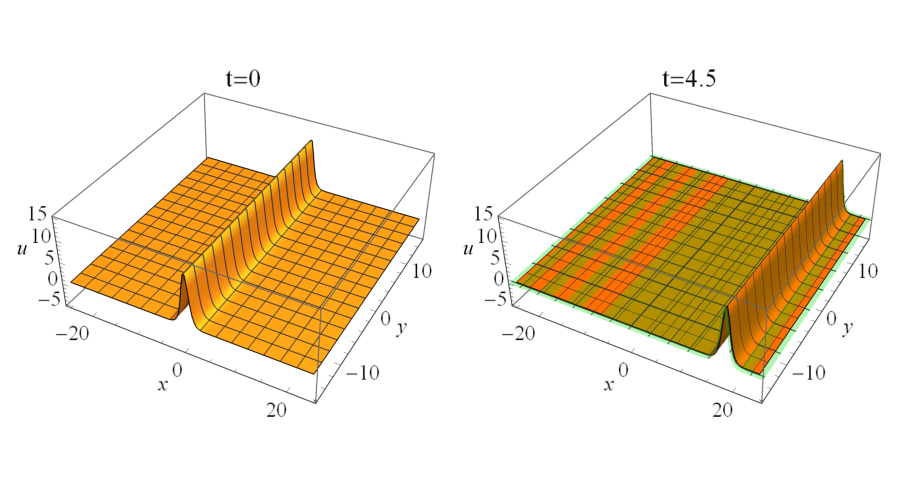
\includegraphics[width=1.0\textwidth]{figex2}
	%\caption{Stable plane wave propagation. The shape and position of the plane wave  solution at $t=4.5$ do correspond for the numerical solution (orange colored) and the analytical one (green colored).}\label{figex2}
	\caption{Устойчивое распространение плоской волны. Форма и положение решения плоской волны при $ t = 4.5 $ действительно соответствуют численному решению (оранжевый цвет) и аналитическому решению (зеленый цвет).}\label{figex2}	
\end{figure}

%Perturbed plane solitary wave soliton is studied using the initial condition developed on the basis of the asymptotic analysis (\ref{stlong}),
Устойчивость солитона в виде плоской уединенной волны исследуется с использованием начального условия, разработанного на основе асимптотического анализа (\ref {stlong}),
\begin{equation}
	\label{kp1ex2}
	u(x,y,0)=12{\text{sech}}^2(x-4t) - 2.4 {\text{cos}} (y) {\text{tanh}} (x) ~{\text{sech}}^2(x),
\end{equation}
%where $f = \pm 3$ is used in Eq. (\ref{kp3gen}).  According to the analytical solution $f=3$ corresponds to the stable case, while $f=-3$ relates to a transverse instability.
где $ f = \pm 3 $ используется в уравнении (\ref {kp3gen}). Согласно аналитическому решению, $ f = 3 $ соответствует устойчивому случаю, а $ f = -3 $ --- поперечной неустойчивости.
\begin{figure}
	\centering
	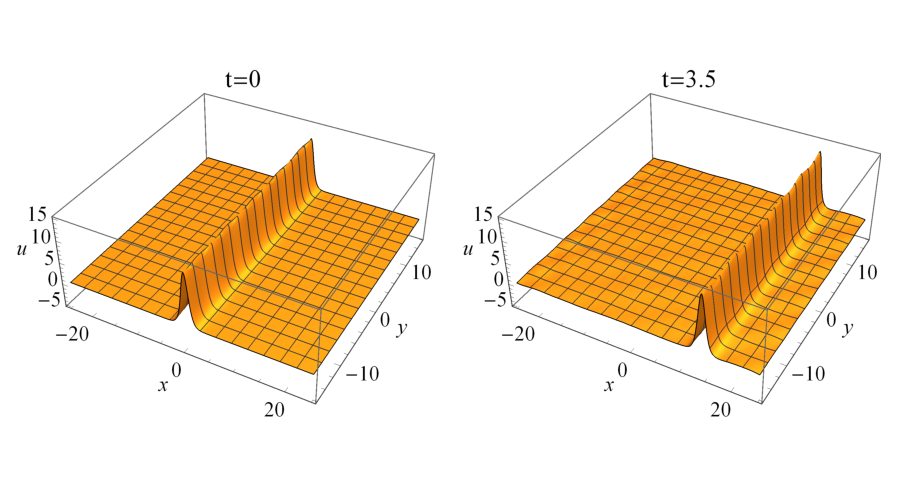
\includegraphics[width=1.0\textwidth]{fig_kp1_stable}
	%\caption{Numerical solution for the initial condition $u(x,y,0)$ for $f=3$.}\label{figex3}
	\caption{Численное решение в случае начального условия $u(x,y,0)$ при $f=3$.}\label{figex3}	
\end{figure}
\begin{figure}
	\centering
	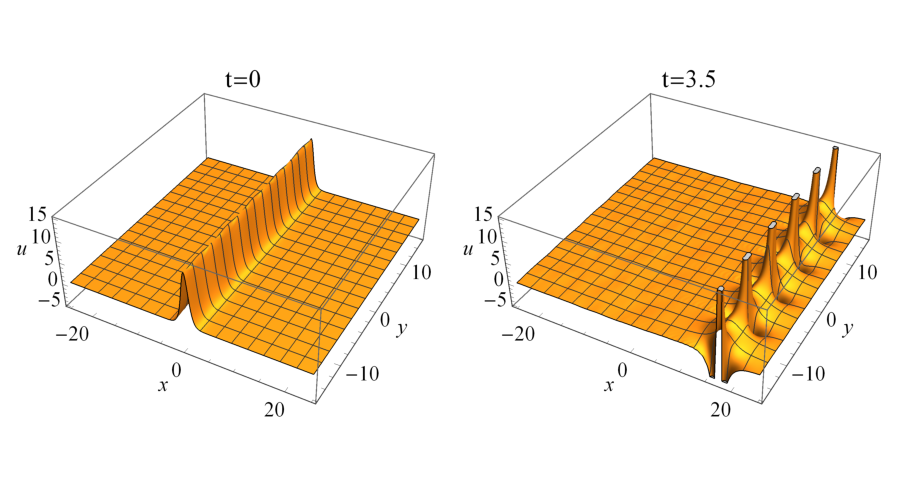
\includegraphics[width=1.0\textwidth]{fig_kp1_frw}
	%\caption{Numerical solution for the initial condition $u(x,y,0)$ for $f=-3$. The interpolation surface of the solution is cut off at $z=15$ in order to save the scale.}\label{figex4}
	\caption{Численное решение в случае начального условия $u(x,y,0)$ при $f=-3$. Поверхность интерполяции решения обрезается на $ z = 15 $ для сохранения масштаба.}\label{figex4}	
\end{figure}
\begin{figure}
	\centering
	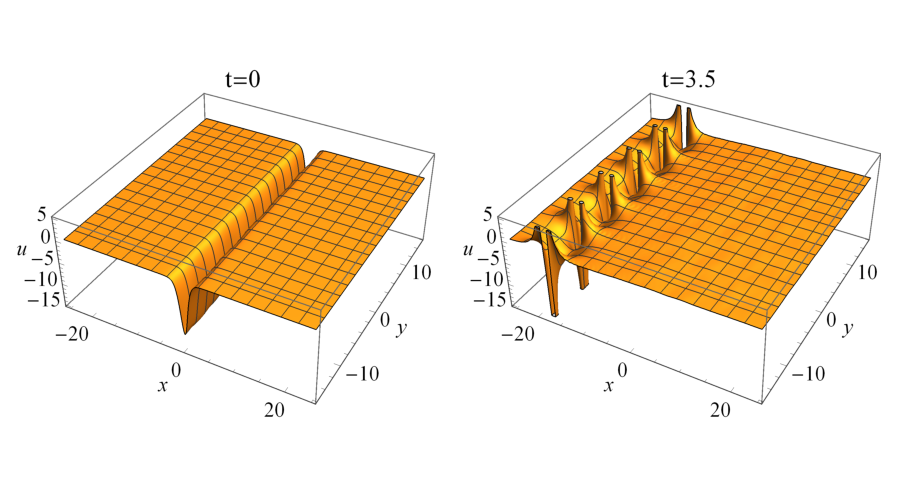
\includegraphics[width=1.0\textwidth]{fig_kp1_inverse}
	%\caption{Numerical solution for the initial condition $-u(x,y,0)$ for $f=3, c_1=-1$. The interpolation surface of the solution is cutted off at $z=-15$ in order to save the scale.}\label{figex44}
	\caption{Численное решение в случае начального условия $-u(x,y,0)$ при $f=-3, c_1=-1$. Поверхность интерполяции решения обрезается на $ z = -15 $ для сохранения масштаба.}\label{figex44}	
\end{figure}

%Comparing Figs.~\ref{figex2},~\ref{figex3} one can see the stable propagation of the plane wave in Fig.~\ref{figex3}  at the initially transversely perturbed plane wave. The wave in both figures propagates keeping its shape and velocity while initial perturbation at the wave in Fig.~\ref{figex3}  dispapear in time.
Сравнивая рис. ~ \ref{figex2}, ~\ref{figex3}, можно увидеть, что в первом случае наблюдается устойчивое распространение плоской волны на рис. ~\ref{figex3}, как и предсказывает теория. В обоих случаях волна распространяется сохраняя свою форму и скорость, при этом в первом случае возмущения исчезают со временем, а во втором --- растут.

%On the contrary, one can see in  Fig.~\ref{figex4} that the initial condition with negative $f$ provides serious transverse variations on the plane wave front. Initial small periodic perturbations suffer an increase in the amplitude and initially almost plane wave evolves into a transversely modulated wave. This happens in an agreement with an analysis. It was noted before that $c_1$ may be negative rather than $f$. However, transformation of variables, $t=-\tau$, $u=-v$, at negative $c_1$ and positive $f$ results in the obtaining equation for $v$ with positive $c_1$ and negative $f$ corresponding to an unstable propagation of negative amplitude wave $u$  (see Fig. ~\ref{figex44}).
Напротив, на рис. ~ \ref{figex4} видно, что начальное условие с отрицательным значением $ f $ приводит к серьезным поперечным изменениям на фронте плоской волны. Начальные малые периодические возмущения претерпевают увеличение амплитуды, и первоначально почти плоская волна превращается в поперечно-модулированную волну. Этот факт находится в соответствии с результатами теоретического анализа. Ранее отмечалось, что $ c_1 $ может быть отрицательным, а $ f $ --- нет. Однако преобразование переменных $ t = - \tau $, $ u = -v $ при отрицательном $ c_1 $ и положительном $ f $ приводит к получению уравнения для $ v $ с положительным $ c_1 $ и отрицательным $ f $, что соответствует неустойчивому распространению волны отрицательной амплитуды $ u $ (см. рис. ~ \ref{figex44}).

%\subsubsection{Numerical results for shear waves equation}
\subsubsection{Численные результаты для уравнения поперечных волн}

%Consider Eq.~(\ref{fkpscheme}) for $p=2$ and $\gamma \ne 0$.   
%For all simulations $N_x = 1025, N_y = 129$, time step $\Delta t = 0.003$ with 2 iterations per step. $N_x$ is chosen to be higher than it was for previous simulations in order to increase the accuracy of evaluation of the term given by Eq.~(\ref{termRY}).
Рассмотрим уравнение ~ (\ref{fkpscheme}) в случае $ p = 2 $ и $ \gamma \ ne 0 $.
Для всех расчетов $ N_x = 1025, N_y = 129 $, временной шаг выбран равным $ \Delta t = 0.003 $ с 2 итерациями на шаг. $ N_x $ выбрано больше, чем было для предыдущих симуляций, чтобы повысить точность оценки члена, задаваемого уравнением ~ (\ref{termRY}).

%The parameters  (\ref{solshearpar}) of exact solution (\ref{solshear}) depend on $m$ responsible for propagation inclined to the $x$ axis and two sets of parameters are possible. Therefore it is of interest to study inclined propagation of shear waves. For this purpose the initial condition is constructed as the sums of three plane wave solitons (\ref{solshear}) (at $t=0$). The distance between them is chosen  larger than their effective length, so the interaction between these solitons is very small. Also the choice of the distance provides periodic conditions for $y$ as it is seen in  Fig.~\ref{figex1025l}.
Параметры (\ref{solshearpar}) точного решения (\ref{solshear}) зависят от $ m $, ответственного за направление распространения волны относительно оси $ x $. При $m \ne 0$ необходимо сохранить условие на периодичность по обеим осям в силу ограничений численной модели. Для этого начальное условие можно построить как сумму трех солитонов плоских волн (\ref{solshear}) (при $ t = 0 $) таким образом, что периодичность сохраняется в обоих направлениях. Очевидно, что такая суперпозиция не является точным решением уравнения. Однако расстояние между солитонами выбрано больше их эффективной длины, поэтому взаимодействие между этими солитонами очень мало, и какое-то достаточно большое время плоские уединенные волны должны продолжать устойчиво распространяться с постоянной скоростью. Также выбор этого расстояния фактически обязывает изменить границы области, чтобы обеспечить периодичность, как это видно на рис. ~ \ref{figex1025l},
%The calculation domain in $x$ is increased in order to avoid the boundary influence. 
$$
L_x = 30 \pi.
$$

\begin{figure}
	\centering
	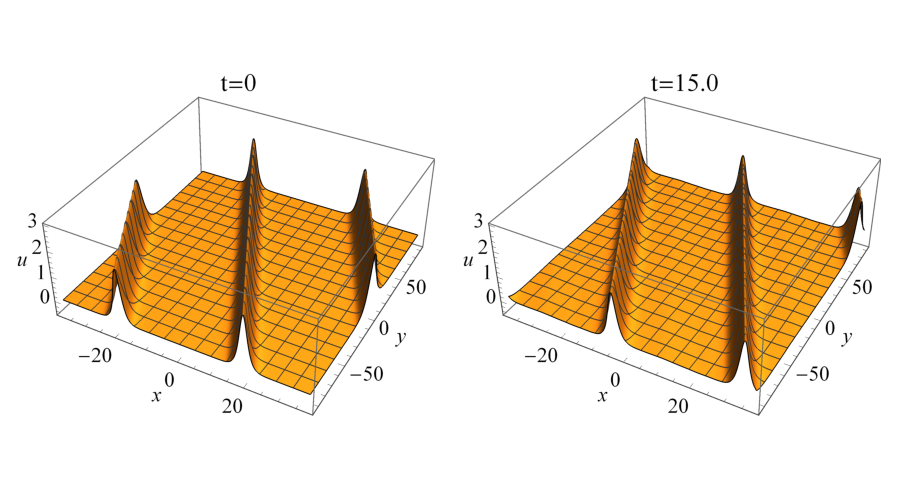
\includegraphics[width=1.0\textwidth]{figex1025l}
	%\caption{Stable inclined plane shear wave propagation. The numerical solution corresponds to the sum of three analytical plane wave  soliton solutions of Eq.~(\ref{kp3gen}) at $t = 15$.} \label{figex1025l}
	\caption{Распространение устойчивой наклонной плоской поперечной волны. Численное решение соответствует сумме трех аналитических солитонных решений плоской волны уравнения .~(\ref{kp3gen}) при $t = 15$.} \label{figex1025l}	
\end{figure}

%The initial condition is
Соответствующее начальное условие,

\begin{equation}
	\label{kp3ex2}
	u(x,y,0) = u_{\text{exact}}~(\xi ) + u_{\text{exact}}~(\xi - 2 L_y \tan \phi) + u_{\text{exact}}~(\xi + 2 L_y \tan \phi),
\end{equation}
%where
где
\begin{equation}
	u_{\text{exact}}~(\xi ) = \frac{A}{\left(Q+{\text{cosh}} (\xi )\right)},
\end{equation}
\[
A=\frac{6 c_1}{\sqrt{6 c_1 c_2+\gamma ^2 m^2}},~Q=\pm \frac{\gamma  m}{\sqrt{6 c_1 c_2+\gamma ^2 m^2}},
\]
\[
\xi = x + m y - V t, \quad V = c_1+f  m^2, \quad m = \tan{\phi}, \quad \phi = 0.2;
\]
\[
c_1 = 1, \quad c_2 = 1, \quad f = 3, \quad \gamma = 2.
\]

%The  results of stable propagation of the inclined plane waves are shown in Fig.~\ref{figex1025l}. One can check that each of inclined solitary wave corresponds to the single wave exact solitary wave solution.
Результаты устойчивого распространения наклонных плоских волн показаны на рис. ~ \ref{figex1025l}. Качественная оценка полученных результатов соответствует ожиданиям. Таким образом, численная схема позволяет оценивать свойства распространения волн в обоих направлениях и может использоваться для изучения поперечной неустойчивости плоских волн, в том числе асимметричных свойств распространения возмущений.

%To study the transverse instability we consider propagation of a single solitary wave along the $x$ axis. The perturbed initial condition is chosen according to the instability analysis of shear waves,
Для исследования поперечной неустойчивости рассматривается распространение одиночной уединенной волны вдоль оси $ x $. Возмущенное начальное условие выбирается следующим образом,
\begin{equation}
	u(x,y,0) = \sqrt{6} ~{\text{sech}}(x)-\sqrt{6}{\text{tanh}} (x) ~{\text{sech}}(x) {\text{cos}} (y),
\end{equation}
%The results are shown in Figs.~\ref{fig_good1},~\ref{fig_good3},~\ref{fig_good2}. 
Результаты расчетов продемонстрированы на рисунках ~\ref{fig_good1},~\ref{fig_good3},~\ref{fig_good2}. 
%The stable case is shown in Fig.~\ref{fig_good1} corresponds to stable case. 
%The stable case is shown in Fig.~\ref{fig_good1}.
Стабильный случай соответствует рисунку ~\ref{fig_good1}.
%One can see that the initial perturbations on the front of the wave decrease while a two-dimensionally periodic tail develops behind the plane strain  solitary wave.
Видно, что начальные возмущения на фронте волны уменьшаются, а за уединенной волной плоской деформации возникает двухмерные периодические возмущения.

\begin{figure}
	\centering
	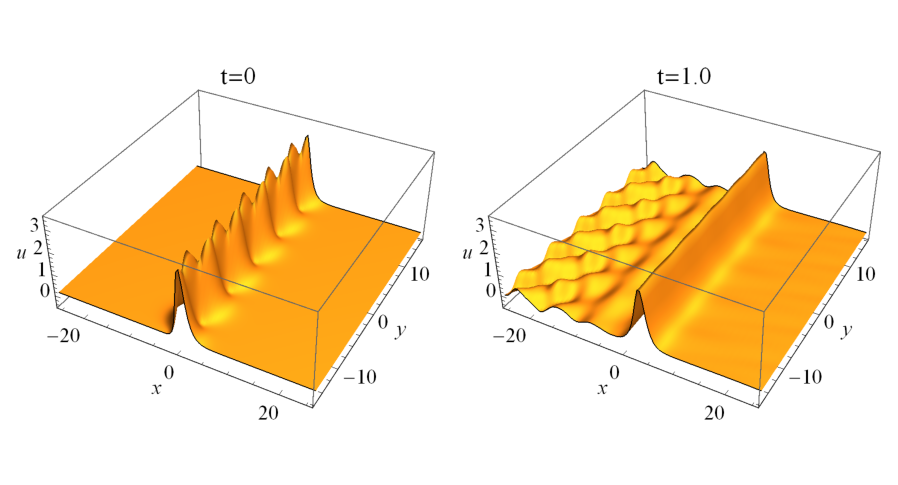
\includegraphics[width=1.0\textwidth]{fig_good1}
	%\caption{Propagation of $u(x,y,0)$ for $f = 3, \gamma = 2$} \label{fig_good1}
	\caption{Распространение поперечно-возмущенной плоской волны. Начальное условие $u(x,y,0)$ при $f = 3, \gamma = 2$} \label{fig_good1}
\end{figure}

\begin{figure}
	\centering
	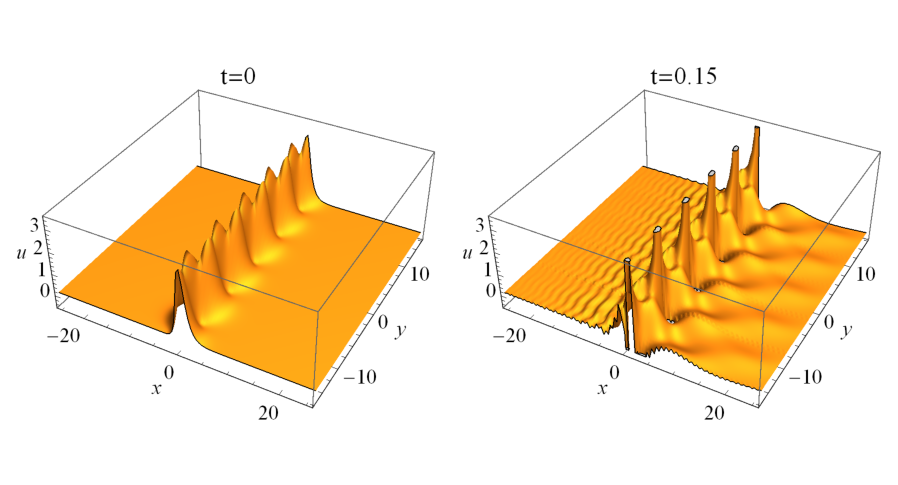
\includegraphics[width=1.0\textwidth]{fig_good3}
	%\caption{Propagation of $u(x,y,0)$ for $f = -3, \gamma = 1$} \label{fig_good3}
	\caption{Распространение поперечно-возмущенной плоской волны. Начальное условие $u(x,y,0)$ при $f = -3, \gamma = 1$} \label{fig_good3}	
\end{figure}

\begin{figure}
	\centering
	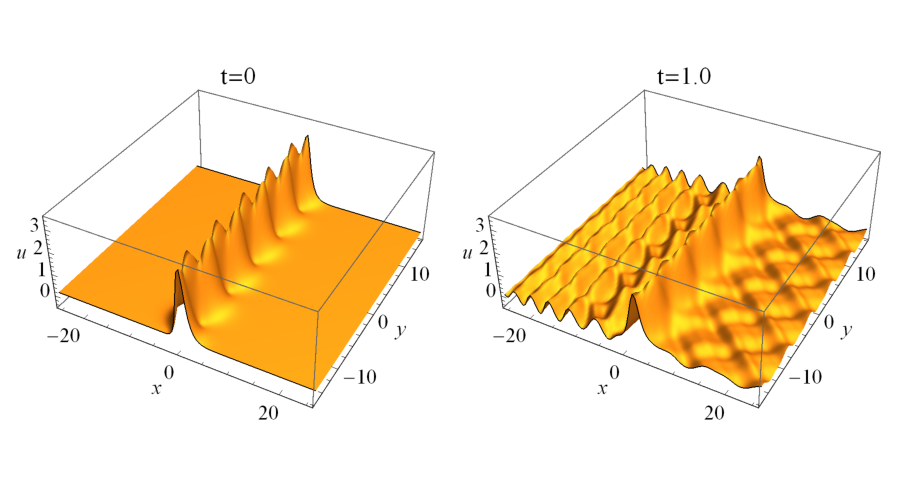
\includegraphics[width=1.0\textwidth]{fig_good2}
	%\caption{Propagation of $u(x,y,0)$ for $f = -3, \gamma = 2$} \label{fig_good2}
	\caption{Распространение поперечно-возмущенной плоской волны. Начальное условие $u(x,y,0)$ при $f = -3, \gamma = 2$} \label{fig_good2}
\end{figure}

%The unstable plane shear wave propagation is shown in  Figs.~\ref{fig_good3}, \ref{fig_good2}. In the former Figure one can see an evolution similar to that found for longitudinal waves: increase in the amplitude and deep transverse modulation of the plane wave front. The latter Figure demonstrates an influence of the value of  $\gamma $ on the transverse instability. The oscillations on the front don't grow anymore while perturbations are developing both before and after the plane wave front.
Распространение неустойчивой плоской поперечной волны показано на рис.~ \ref {fig_good3}, \ref{fig_good2}. На первом рисунке можно увидеть эволюцию, аналогичную той, что наблюдается для продольных волн: увеличение амплитуды и глубокая поперечная модуляция фронта плоской волны. Последний рисунок демонстрирует влияние значения $ \gamma $ на поперечную неустойчивость. Колебания на фронте больше не нарастают, а возмущения развиваются как до, так и после фронта плоской волны.

\fixme{Добавить более корректное обобщение численной схемы, так как текущая пренебрегает некоторыми условиями, о которых нигде не сказано. В таком случае ее можно будет представить к защите.}


\subsection{Начальные условий, локализованные в обоих направлениях}
%\textbf{Equation for shear strains and its solution}

%\fixme{Перевести, отмасштабировать рисунки на textwidth, убрать multiple definitions}
%%The governing equation for shear waves reads \cite{porkros, PorOsAnt2020}
%Для дальнейшего численного анализа уравнения (\ref{nonkp}), (\ref{kpsh}) удобно представить в новых переменных следующем виде
%\begin{equation}
%	v_{xt} +c_1~F_{xxxx}+ c_2~ v_{x}^2~ v_{xx}+\lambda v_{yy}+\gamma~v_{y}~ v_{xx}~=~0, \label{kpsh222}
%\end{equation}
%где $c_i$, $\lambda$, $\gamma$ --- константы. 
%
%%One can see that Eq. (\ref{kpsh222}) is not invariant under the transformation $y\rightarrow -y$.  Consider its plane traveling wave solution depending only on the phase variable $\xi=x+ m y-V t$ and assume that $u=v_x$.
%Можно видеть, что уравнение (\ref {kpsh222}) не инвариантно относительно преобразования $ y \rightarrow -y $. Рассмотрим его решение в виде плоской бегущей волны, зависящее только от фазовой переменной $ \xi = x + m y-V t $, и предположим, что $ u = v_x $.
%%The solution, obtained by using direct integration, reads
%Решение, полученное с помощью прямого интегрирования аналогично \ref{solshear}, в новых переменных имеет вид
%\begin{equation}
%	u=\frac{A}{Q+{\text{cosh}}( \beta \xi)},\label{solshear2}
%\end{equation}
%%where
%где
%\begin{equation}
%	A=\pm \frac{6c_1 \beta^2}{\sqrt{\gamma^2 m^2+6 c_1 c_2 \beta^2}}, 
%	Q_{\pm}=\pm\frac{\gamma m }{\sqrt{\gamma^2 m^2+6 c_1 c_2 \beta^2}},  V=\beta^2 c_1+m^2 \lambda . \label{solshearpar2}
%\end{equation}
%%We consider only bounded solutions when $Q<1$. This is guaranteed if $c_1 c_2>0$, and the solutions with both $Q_{+}$  and $Q_{-}$ being bounded. Otherwise only positive $Q_{\pm}$ give rise to a bounded solution.  The sign of $Q$ depends on the sign of the parameter $m$ responsible for the angle of the wave front propagation relative to the $x$- axis and the sign of the denominator.  However, the presence of $\pm$ in the expression for $Q_{\pm}$ discards the dependence on the sign of $m$. The sign of the amplitude $A/(Q+1)$ of the bounded solution is not sensitive to the sign of $m$.
%В новых переменных, решение ограничено также в случае $ Q < 1 $. Последнее гарантируется, если $ c_1 c_2> 0 $ и решения с $ Q_ {+} $ и $ Q_ {-} $ ограничены. В противном случае только положительное значение $ Q_ {\pm} $ приводит к ограниченному решению. Знак $ Q $ зависит от знака параметра $ m $, отвечающего за угол распространения волнового фронта относительно оси $ x $, и знака знаменателя. Однако наличие $ \pm $ в выражении для $ Q_ {\ pm} $ снимает зависимость от знака $ m $. Знак амплитуды $ A / (Q + 1) $ ограниченного решения не чувствителен к знаку $ m $.
%%% уже объяснено ранее ^^^

%%For the wave propagating along $x$ axis we have $m=0$ and $Q=0$. Then the familiar solitary wave solution to the modified Korteweg-de Vries equation appears from (\ref{solshear2}),
%Частный случай уединенной волны, распространяющейся строго вдоль оси $x$, аналогичный описываемому уравнением \ref{qp}, требует $m=0$ и $Q=0$ и выражается следующим образом,
%\begin{equation}
%	q_m=\pm \frac{6c_1\beta}{\sqrt{6 c_1 c_2}}{\text{cosh}}^{-1}(\beta \xi). \label{qp2}
%\end{equation}
%Решение существует только при $c_1 c_2>0$. 

%\section{Numerical study of nonlinear shear strains localization}
%Let us re-write Eq. (\ref{kpsh222}) through the shear strain, 
%\begin{equation}
%	\label{kp3gen}
%	\partial_x\left(\partial_t u+c_1 \partial_{xxx} u+\frac{c_2 }{3}\partial_x u^{3}\right)+\lambda \partial_{yy} u+\gamma \partial_x\left(\partial_x u \int_{-\infty}^x \partial_y u \, dx'\right)=0.
%\end{equation}

%The Fourier spectral method is used here to solve Eq.~(\ref{kp3gen}) numerically. More detailed information about the method can be found in \cite{PorOsAnt2020}.
%In all the simulations we put $p=2$, $c_1 = 1$, $c_2 = 1$ and $f = 3$. The initial condition is assumed as
Были рассмотрены случаи распространения плоских волн, не ограниченных в направлении $y$. Однако интерес могут также представлять и полностью локализованные начальные условия, а также влияние параметров модели на их эволюцию. Для численного исследования таких волн, изначально локализованных в обоих направлениях и описываемых уравнением (\ref{kp3gen}), выберем начальное условие следующего вида,
\begin{equation}\label{init}
	u_0 = \frac{\sqrt{6}\;\mathrm{sech}(X)}{10^{-8} \mathrm
		{cosh} (0.6 Y)+1},
\end{equation}
$$
X = a_1 x + b_1 y, ~Y = a_2 x + b_2 y,
$$
где $a_1, b_1, a_2, b_2$ --- константы, определяющие угол между осью $x$ и направлением, перпендикулярным фронту волны. Выражения для $X, Y$ и соответствующих наборов коэффициентов для разных случаев расчета представлены в таблице ~\ref{table1}. Профиль такого вида представляет собой плоскую уединенную волну, гладко ограниченную в направлении, перпендикулярном фронту волны. 

Константы уравнения (\ref{kp3gen}) определяются следующим образом,
\[
p=2, ~c_1 = 1, ~c_2 = 1, ~f = 3.
\]
Такой выбор соответствует уравнению (\ref{kpsh}), описывающему распространение сдвиговых волн деформации. 

Ниже представлены результаты численного счета для разных случаев, рис.~\ref{fig1}, \ref{fig2}, \ref{fig3}, \ref{fig4}. Для всех случаев время моделирования и границы расчетной области выбраны одинаковыми.

%The values of $X, Y$ and $\gamma$ are varied as shown in Table~\ref{table1}.
\begin{figure}[h]
	\begin{center}
		\begin{tabular}{cc}
			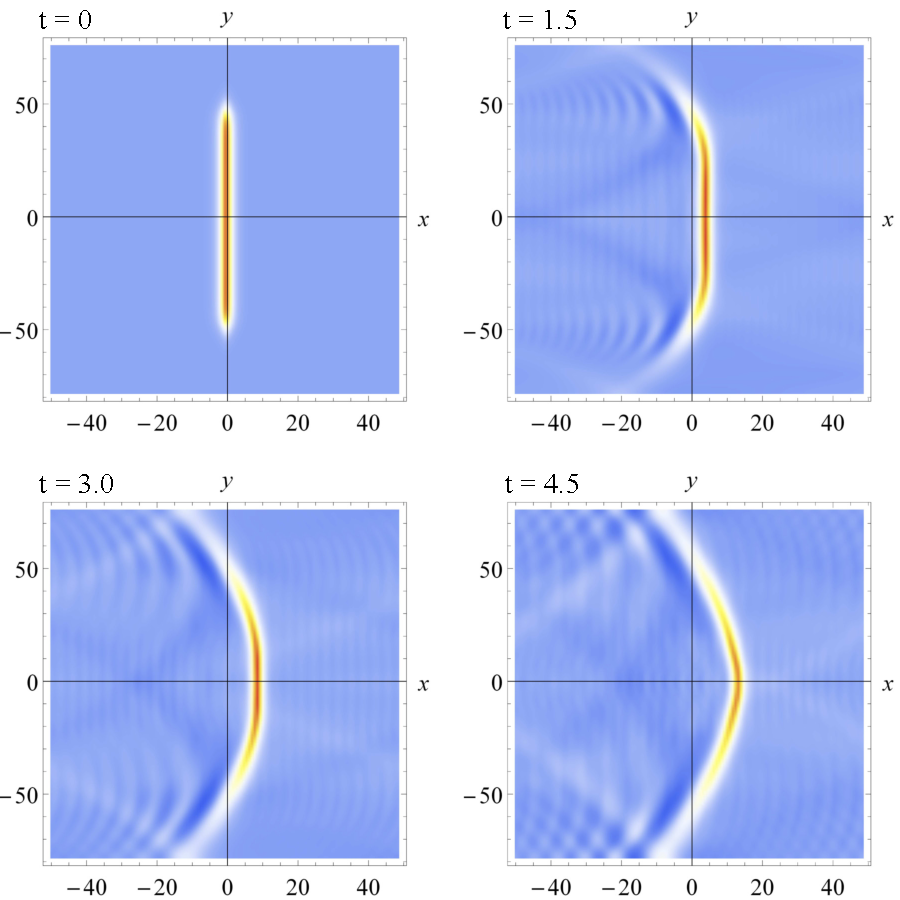
\includegraphics[width=0.85\textwidth]{fig1t.pdf} & 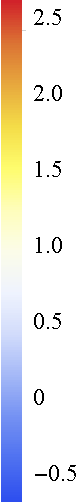
\includegraphics[width=0.08\textwidth]{palette.pdf}
		\end{tabular}
		%\caption{Evolution of the shear strain wave(\ref{init}) in Case 1.}\label{fig1}
		\caption{Эволюция решения для начального условия, определяемого уравнением (\ref{init}) в случае 1.}\label{fig1}
	\end{center}
\end{figure}
\begin{figure}
	\begin{center}
		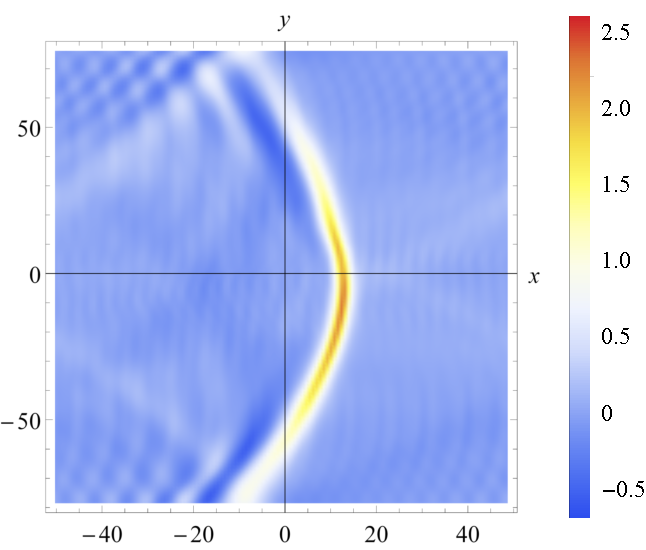
\includegraphics[width=0.75\textwidth]{fig2_instead.pdf} 
		%\caption{Transformation to an asymmetric profile in Case 2 at t = 4.5.}\label{fig2}
		\caption{Асимметричность профиля, возникающая в случае 2 при $t = 4.5$.}\label{fig2}		
	\end{center}
\end{figure}
\begin{figure}
	\begin{center}
		\begin{tabular}{cc}
			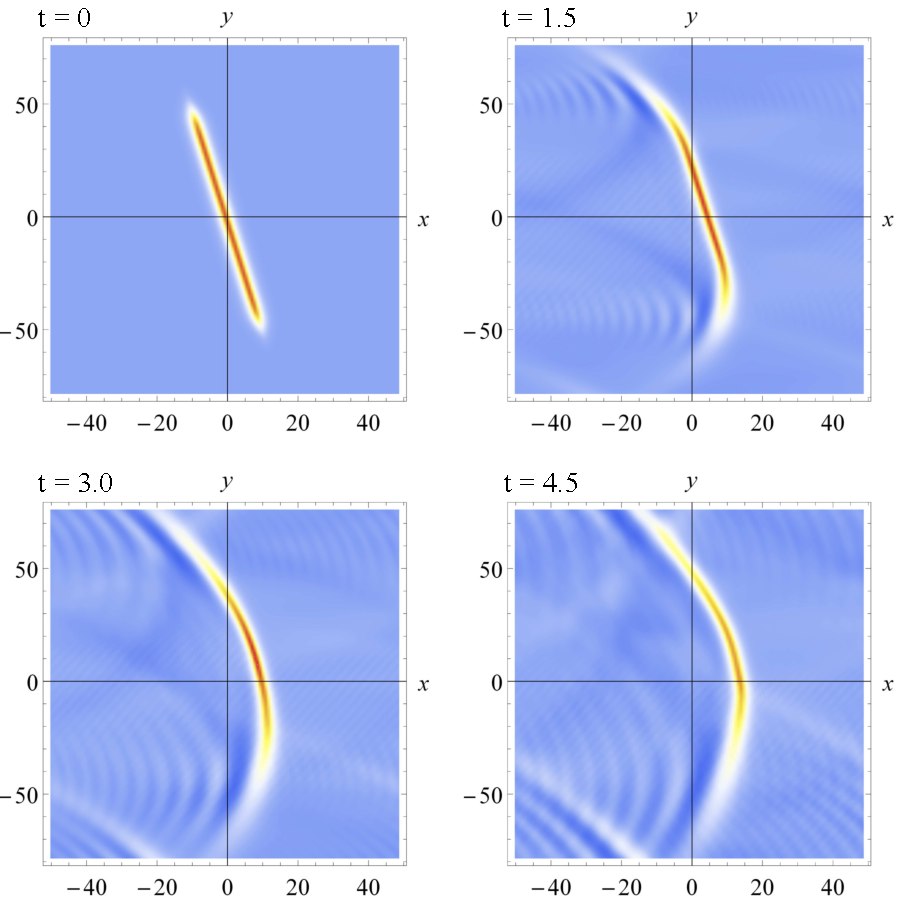
\includegraphics[width=0.85\textwidth]{fig3t.pdf} & 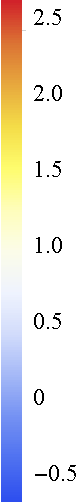
\includegraphics[width=0.08\textwidth]{palette.pdf}
		\end{tabular}
		%\caption{Asymmetry for the initial condition corresponding to Case 3.}\label{fig3}
		\caption{Эволюция решения для начального условия, определяемого уравнением (\ref{init}) в случае 3.}\label{fig3}
	\end{center}
\end{figure}

\begin{figure}
	\begin{center}
		\begin{tabular}{cc}
			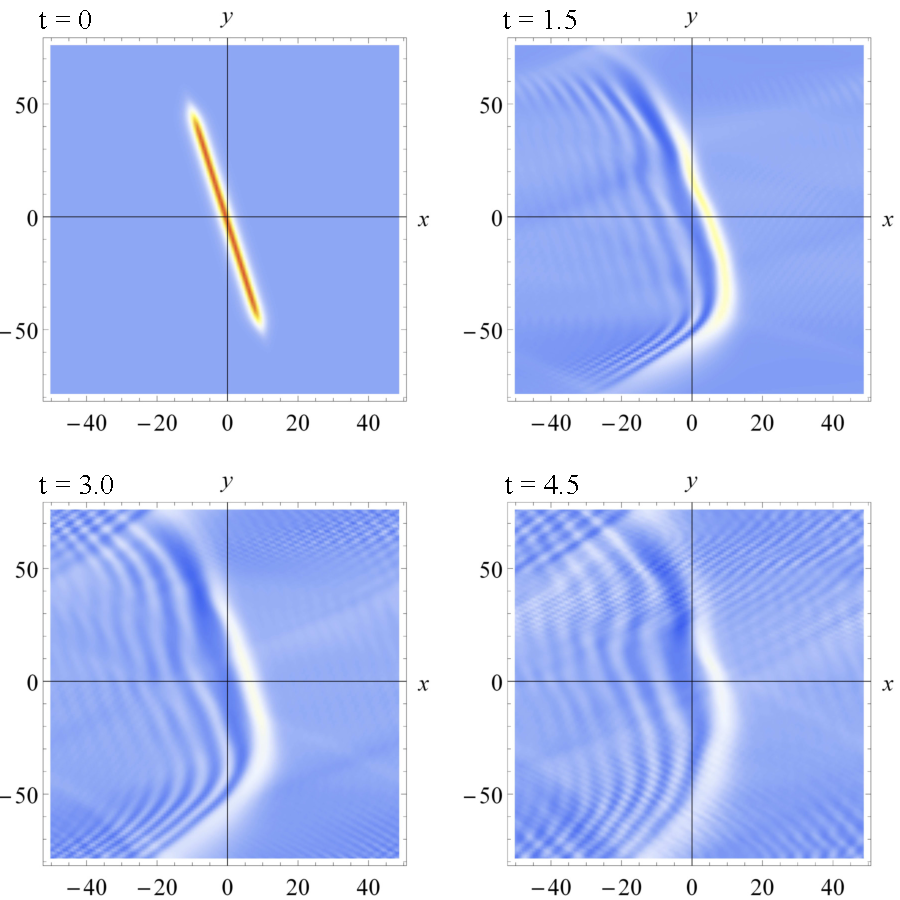
\includegraphics[width=0.85\textwidth]{fig4t.pdf} & 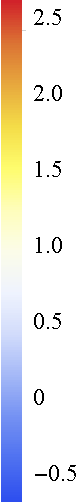
\includegraphics[width=0.08\textwidth]{palette.pdf}
		\end{tabular}
		%\caption{Scattering of the initial condition corresponding to Case 4.}\label{fig4}
		\caption{Эволюция решения для начального условия, определяемого уравнением (\ref{init}) в случае 4.}\label{fig4}
	\end{center}
\end{figure}
\begin{table}[h!]
	\centering
	\begin{tabular}{|l|l|l|l|}
		\hline
		& $X$ & $Y$ & $\gamma$\\ \hline
		%Case 1 &  $x$   & $y$  & 0 \\ \hline
		%Case 2 &   $x$   &   $y$ & 1 \\ \hline
		%Case 3 &  $x \cos (0.2 )+y \sin (0.2 )$   &   $x \cos (0.2 )+y \sin (0.2 )$ & 1\\ \hline
		%Case 4 &   $x \cos (0.2 )+y \sin (0.2 )$  &  $x \cos (0.2 )+y \sin (0.2 )$  & 5\\ \hline
		Случай 1 &  $x$   & $y$  & 0 \\ \hline
		Случай 2 &   $x$   &   $y$ & 1 \\ \hline
		Случай 3 &  $x \cos (0.2 )+y \sin (0.2 )$   &   $x \cos (0.2 )+y \sin (0.2 )$ & 1\\ \hline
		Случай 4 &   $x \cos (0.2 )+y \sin (0.2 )$  &  $x \cos (0.2 )+y \sin (0.2 )$  & 5\\ \hline
		
	\end{tabular}
%	\caption{Expressions of $X, Y$ for the initial conditions.}\label{table1}
	\caption{Выражения для коэффициентов $X, Y$ в начальных условиях, определяемым уравнением \ref{init}, для разных расчетных случаев.}\label{table1}
\end{table}


%\textbf{Case 1}. In Fig.~\ref{fig1} the symmetric relative to the $x$-axis propagation of the strain wave (\ref{init}) is shown. The curvature of the wave profile develops in time and a scattering of the wave happens behind the curved wave front. The amplitude and the velocity of the wave  decrease in  time. 
%
%\textbf{Case 2}. The initial profile suffers from asymmetric variations relatively to the $x$-axis, see Fig. \ref{fig2}. The highest  amplitude is not reached on the $Ox$ axis. However, changing the sign of $\gamma$ does not provide additional non-symmetry.   
%
%\textbf{Case 3}. The role of quadratic nonlinearity on the initially inclined wave is shown in Fig. \ref{fig3}. It is quite similar to what is shown in Fig.~\ref{fig2}. The presence of the nonlinear term changes the direction of wave propagation in the similar way as in Case 2. The amplitude and velocity  also decrease in time.
%
%\textbf{Case 4}. One can see in Fig. \ref{fig4} that an increase in the value of $\gamma$ results in a  scattering behind the wave front.

\textbf {Случай 1}. На рис.~\ref {fig1} представлены численные результаты, предсказывающие симметричное относительно оси $ x $  распространение волны деформации (\ref {init}). Кривизна профиля волны развивается со временем, и происходит рассеяние волны за искривленным фронтом волны. Амплитуда и скорость волны уменьшаются со временем.

\textbf {Случай 2}. Начальный профиль подвергается асимметричными изменениями относительно оси $ x $, см. рис.~\ref{fig2}. На оси $ Ox $ наибольшая амплитуда не достигается. Однако изменение знака $ \gamma $ не дает дополнительной несимметрии.

\textbf {Случай 3}. Роль квадратичной нелинейности на изначально повернутой относительно оси $x$ волне демонстрируется на рис.~\ref{fig3}. Эволюция схожа с той, что показано на рис.~\ref {fig2}. Наличие нелинейного члена изменяет направление распространения волны аналогично случаю 2. Амплитуда и скорость также уменьшаются со временем.

\textbf {Случай 4}. Согласно численным результатам, представленным на рис.~\ref {fig4} видно, что дальнейшее увеличение значения $ \gamma $ приводит к рассеянию за фронтом и быстрому распаду изначально локализованной волны.

\fixme{Какой-нибудь вывод промежуточный?}

%\section{Conclusions}
\section{Заключение}

\fixme{Доделать...}

%The asymptotic technique presented in this paper allows to reduce the coupled nonlinear continuum equations of 2D crystal lattices to a single nonlinear equation for strain waves, which allows to analyze only relevant terms in the new equations.
%Two types of lattices were considered: the generalized square lattice and the graphene lattice (the model is based on a consideration of two interacting sub-lattices with both translational and angular interactions being taken into account), and the governing two-dimenisonal equations for longitudinal and shear strain waves. Their exact plane wave solutions and their transverse stability have been revealed  in  numerical simulations.

%Numerical simulations confirm  that the angular stiffness in the original discrete model gives rise to various types of nonlinear waves localization depending on the coefficients values. Previous studies of the lattices of another structure revealed important variations in the governing equation from that of the longitudinal waves \cite{porkros}.
%Extended interactions in the square lattice firstly produce additional extrema in the dispersion curve for linear longitudinal plane waves. They have a significant influence on the auxetic behavior of the material. One can note that the one-dimensional limits of the equations for longitudinal and shear waves differ only by nonlinear terms (quadratic or cubic) while two-dimensional consideration results in different transverse variation terms which are nonlinear for shear waves contrary to the linear term for longitudinal waves. Moreover, the sign of the coefficients in the governing equations may vary more for shear waves descriptions. It results in different stability criteria for longitudinal and shear localized plane strain waves. 

%This, in turns it allows us to predict different scenario of the wave amplification and localization due toa  transverse instability caused by the values of the coefficients of rigidity. In the stable case of the Kadomtsev-Petviashvili equation (\ref{kp}) two-dimensional localized wave amplification happens due to instability, see Figs. \ref{figex4}, \ref{figex44}. An unstable case of Eq. (\ref{kp}) also results in the transverse periodic modulation of the plane wave. Figure  \ref{figex4} demonstrated classical result for the corresponding negative sign at the term with derivatives with respect to $y$. However, this case is not realized for description of our lattice while the negative sign at the dispersion term can be achieved. This results in the dynamics shown in Fig.  \ref{figex44}. The new results concern the transverse instability of nonlinear shear waves, see Figs. ~\ref{fig_good3}, \ref{fig_good2} which is different from that of longitudinal waves.
%The comparison of the numerical results for shear waves gives an explanation, how the coefficient at the quadratic nonlinearity influences the inclined plane solitary wave  propagation and the transverse instability.  

%One of the potential extensions of this study is a  short-range wave continualization. Previously it was studied for a hexagonal lattice in Refs. \cite{PorBer, PorBer2} where new model modulation two-dimensional equations were obtained. Also, nonlocal interactions will be of interest, in particular, utilization of the method of using shift operators \cite{Mich} for obtaining two-dimensional model equations for dynamical processes in nonlocal square lattice will be considered in the nearest future.
%Another extension of the model concerns an inclusion of the geometrical nonlinearity in the discrete model like it was done, e.g., in (\cite{karima}).
%Furthermore, along with the geometrical nonlinearity and weakly transversely perturbed shear waves, the study can be extended to the case of nonlinear translational stiffnesses examination.

%Асимптотическая техника, представленная в этой статье, позволяет свести связанные нелинейные уравнения континуума двумерных кристаллических решеток к одному нелинейному уравнению для волн деформации, что позволяет анализировать только соответствующие члены в новых уравнениях.
%%%\fixme{Были рассмотрены два типа решеток: обобщенная квадратная решетка и решетка графена (модель основана на рассмотрении двух взаимодействующих подрешеток с учетом как поступательного, так и углового взаимодействия) и определяющие двумерные уравнения для продольных и волны сдвига деформации}. Их точные решения в виде плоских волн и их поперечная устойчивость были выявлены в ходе численного моделирования.
Проведены численные исследования модели обобщенной квадратной решетки, рассматривающей взаимодействие подрешеток с учетом как поступательного, так и углового взаимодействия, задаваемой определяющими двумерными уравнения для продольных и сдвиговых волн деформации. Была представлен численный метод, позволяющий воспроизводить точные решения в виде плоских волн, исследовать свойства их поперечной устойчивости, а также моделировать эволюцию волн деформации при различных локализованных начальных условиях.

Численное моделирование подтверждает, что угловая жесткость в исходной дискретной модели приводит к различным типам локализации нелинейных волн в зависимости от значений коэффициентов. Предыдущие исследования решеток другой структуры выявили важные отличия основного уравнения модели и уравнения для продольных волн \cite{porkros}.
Расширение взаимодействия в квадратной решетке создают дополнительные экстремумы на дисперсионной кривой для линейных продольных плоских волн. 
%Они оказывают значительное влияние на ауксетическое поведение материала. Можно отметить, что одномерные пределы уравнений для продольных и поперечных волн отличаются только нелинейными членами (квадратичными или кубическими), в то время как двумерное рассмотрение приводит к различным членам поперечной вариации, которые являются нелинейными для поперечных волн в отличие от линейного члена для продольные волны. 
Коэффициенты в определяющих уравнениях могут быть разных знаков при описании поперечных волн в зависимости от коэффициентов основного уравнения модели. Это приводит к различным критериям устойчивости продольных и сдвиговых локализованных волн плоской деформации, что подтверждается численными результатами.

Таким образом, представленная численная модель позволяет прогнозировать различные сценарии усиления и локализации волн из-за поперечной неустойчивости, вызванной значениями коэффициентов жесткости. В устойчивом случае уравнения Кадомцева-Петвиашвили (\ref {kp}) двумерное локализованное усиление волн происходит из-за неустойчивости, см. рисунки \ref {figex4}, \ref {figex44}. Неустойчивый случай уравнения (\ref {kp}) также приводит к поперечной периодической модуляции плоской волны. На рисунке \ref {figex4} показан классический результат для соответствующего отрицательного знака у члена с производными по $ y $. Однако этот случай не реализуется для описания рассматриваемой модели, в то время как дисперсионный член может быть отрицательным. Это приводит к динамике, показанной на рис. \ref{figex44}. Новые результаты получены для поперечной неустойчивости нелинейных поперечных волн, см. рисунки ~ \ref {fig_good3}, \ref{fig_good2}, вид которой отличается от продольных волн. Сравнение численных результатов для поперечных волн дает объяснение, каким образом коэффициент при квадратичной нелинейности влияет на распространение плоских уединенных волн и поперечную неустойчивость. Также с помощью численной модели продемонстрирована возможность оценить влияние параметров решетки на эволюцию волн, изначально локализованных в обоих направлениях, что может дать развитие для будущих исследований.
           % Глава 3
%\include{Dissertation/part1}           % Глава 1 - template
%\include{Dissertation/part2}           % Глава 2 - template
%\include{Dissertation/part3}           % Глава 3 - template
\chapter*{Заключение}                       % Заголовок
\addcontentsline{toc}{chapter}{Заключение}  % Добавляем его в оглавление

%% Согласно ГОСТ Р 7.0.11-2011:
%% 5.3.3 В заключении диссертации излагают итоги выполненного исследования, рекомендации, перспективы дальнейшей разработки темы.
%% 9.2.3 В заключении автореферата диссертации излагают итоги данного исследования, рекомендации и перспективы дальнейшей разработки темы.
%% Поэтому имеет смысл сделать эту часть общей и загрузить из одного файла в автореферат и в диссертацию:

Основные результаты работы заключаются в следующем.
%% Согласно ГОСТ Р 7.0.11-2011:
%% 5.3.3 В заключении диссертации излагают итоги выполненного исследования, рекомендации, перспективы дальнейшей разработки темы.
%% 9.2.3 В заключении автореферата диссертации излагают итоги данного исследования, рекомендации и перспективы дальнейшей разработки темы.

%\fixme{Из реферата по философии науки... Нужно исправить и дополнить.}

%В ходе проделанной работы были успешно изучены вопросы истории и методологии исследования нелинейных волновых процессов, было уделено необходимое внимание истории развития методов управления линейными и нелинейными механическими системами, при этом были подробно рассмотрены вопросы о применимости разрабатываемого математического аппарата в ходе исследовательской работы, с акцентом на методы исследования тех областей науки и техники, к которым он будет применяться в перспективе.
%Было получено полноценное представление об истории развития науки о нелинейных волнах, рассмотрены трудности, с которыми сталкивались ученые при построении новых теорий, уделено необходимое внимание появившимся в ходе этого развития новых методов исследования. В рамках данной работы также были изучены современные подходы к управлению нелинейными системами, что несомненно будет полезно для дальнейшей исследовательской работы. Таким образом, все поставленные цели работы были успешно выполнены.

\begin{enumerate}
  \item На основе анализа существующей литературы по тематике исследования были выбраны и сформулированы основные цели работы, поставлены задачи для их решения, обоснована их актуальность, практическая значимость, а также дальнейшие перспективы для развития.
  \item Разработаны модельные уравнения движения для слоя с заданными граничными условиями и видом нелинейной функции потенциальной энергии, исследована возможность управления волновыми процессами в такой механической системе по схеме скоростного градиента и определены границы применимости. 
  \item Разработан спектральный метод решения обобщенного уравнения Кадомцева-Петвиашвили с дополнительным интегральным слагаемым, описывающего распространение волн в двумерных обобщенных решетках. С помощью полученного метода численно продемонстрированы свойства устойчивости плоских волн разных типов, предсказанные аналитически. 
  \item Численно исследованы свойства распространения и генерации гармонических волн для модели метаматериала <<масса-в-массе>> в условиях наличия запрещенной зоны при различных параметрах системы. 
\end{enumerate}


%Последний параграф может включать благодарности.  
В заключение автор
выражает благодарность и большую признательность научному руководителю
Порубову~А.\,В. за поддержку, помощь, обсуждение результатов и~научное
руководство. Также автор благодарит %Сидорова~А.\,А. и~Петрова~Б.\,Б.
%за помощь в~работе с~образцами, Рабиновича~В.\,В. за предоставленные
%образцы и~обсуждение результатов, Занудятину~Г.\,Г. и 
авторов шаблона
*Russian-Phd-LaTeX-Dissertation-Template* за~помощь в оформлении
диссертации. Автор также благодарит много разных людей
и~всех, кто сделал настоящую работу автора возможной.
      % Заключение
%\include{Dissertation/acronyms}        % Список сокращений и условных обозначений
%\include{Dissertation/dictionary}      % Словарь терминов
\include{Dissertation/references}      % Список литературы
%\include{Dissertation/lists}           % Списки таблиц и изображений (иллюстративный материал)

\setcounter{totalchapter}{\value{chapter}} % Подсчёт количества глав

%%% Настройки для приложений
\appendix
% Оформление заголовков приложений ближе к ГОСТ:
\setlength{\midchapskip}{20pt}
\renewcommand*{\afterchapternum}{\par\nobreak\vskip \midchapskip}
\renewcommand\thechapter{\Asbuk{chapter}} % Чтобы приложения русскими буквами нумеровались

%\include{Dissertation/appendix}        % Приложения

\setcounter{totalappendix}{\value{chapter}} % Подсчёт количества приложений

\end{document}
